\documentclass[12pt,]{article}
%\usepackage{lmodern}  Melissa removed to deal with font rendering issue
\usepackage{amssymb,amsmath}
\usepackage{ifxetex,ifluatex}
\usepackage{fixltx2e} % provides \textsubscript

%Melissa removed the following section to deal with font rendering issue
%\ifnum 0\ifxetex 1\fi\ifluatex 1\fi=0 % if pdftex
%  \usepackage[T1]{fontenc}
%  \usepackage[utf8]{inputenc}
%%\else % if luatex or xelatex
%  \ifxetex
%    \usepackage{mathspec}
%  \else
%    \usepackage{fontspec}
%  \fi
%  \defaultfontfeatures{Ligatures=TeX,Scale=MatchLowercase}
%  \newcommand{\euro}{€}
%%%%%%\fi

% use upquote if available, for straight quotes in verbatim environments
\IfFileExists{upquote.sty}{\usepackage{upquote}}{}
% use microtype if available
\IfFileExists{microtype.sty}{%
\usepackage{microtype}
\UseMicrotypeSet[protrusion]{basicmath} % disable protrusion for tt fonts
}{}
\usepackage[margin=1in]{geometry}
\usepackage{hyperref}
\PassOptionsToPackage{usenames,dvipsnames}{color} % color is loaded by hyperref
\hypersetup{unicode=true,
            pdftitle={Status of A Fish (Sebastes yourfish) Off the U.S. Pacific Coast in 2017},
            pdfborder={0 0 0},
            breaklinks=true}
\urlstyle{same}  % don't use monospace font for urls
\usepackage{graphicx,grffile}
\makeatletter
\def\maxwidth{\ifdim\Gin@nat@width>\linewidth\linewidth\else\Gin@nat@width\fi}
\def\maxheight{\ifdim\Gin@nat@height>\textheight\textheight\else\Gin@nat@height\fi}
\makeatother
% Scale images if necessary, so that they will not overflow the page
% margins by default, and it is still possible to overwrite the defaults
% using explicit options in \includegraphics[width, height, ...]{}
\setkeys{Gin}{width=\maxwidth,height=\maxheight,keepaspectratio}
\setlength{\parindent}{0pt}
\setlength{\parskip}{6pt plus 2pt minus 1pt}
\setlength{\emergencystretch}{3em}  % prevent overfull lines
\providecommand{\tightlist}{%
  \setlength{\itemsep}{0pt}\setlength{\parskip}{0pt}}
\setcounter{secnumdepth}{5}

%%% Use protect on footnotes to avoid problems with footnotes in titles
\let\rmarkdownfootnote\footnote%
\def\footnote{\protect\rmarkdownfootnote}

%%% Change title format to be more compact
\usepackage{titling}

% Create subtitle command for use in maketitle
\newcommand{\subtitle}[1]{
  \posttitle{
    \begin{center}\large#1\end{center}
    }
}

\setlength{\droptitle}{-2em}
  \title{Status of A Fish (\emph{Sebastes yourfish}) Off the U.S. Pacific Coast
in 2017}
  \pretitle{\vspace{\droptitle}\centering\huge}
  \posttitle{\par}
  \author{}
  \preauthor{}\postauthor{}
  \date{}
  \predate{}\postdate{}


% This file contains all of the LaTeX packages you may need to compile the document
% Documentation for each package can be found onlines
\usepackage{tabularx}                                             % table environment providing flexibility
\usepackage{caption}                                              % for creating captions  
\usepackage{longtable}                                            % allows tables to span multiple pages
\usepackage{rotating}                                             % allows for sideways tables
\usepackage{float}                                                % floating environments; may not need in rmarkdown
\usepackage{placeins}                                             % keeps floats from moving
\usepackage{indentfirst}                                          % indents first paragraph of a section
\usepackage{mdwtab}                                               % continued float multi-page figure
\usepackage{enumerate}                                            % create lists
\usepackage{hyperref}                                             % highlight cross references
\hypersetup{colorlinks=true, urlcolor=blue, linktoc=page, linkcolor=blue, citecolor=blue} %define referencing colors
%\usepackage{makebox}                                             % make boxes around text
\usepackage[usenames,dvipsnames]{xcolor}                          % color name options
%\usepackage[space]{grffile}                                      % spaces in file name path
\usepackage{soul}                                                 % highlight text
\usepackage{enumitem}                                             % numbered lists
\usepackage{lineno}                                               % Line numbers; comment out for final
\usepackage{upquote}                                              % produce grave accent in latex
\usepackage{verbatim}                                             % produces verbatim results
\usepackage{fancyvrb}                                             % verbatim in a box
%\usepackage{draftwatermark}                                      % places Draft watermark in background; comment out for final
\usepackage{textcomp}                                             % fixes error with packages interfering
\usepackage{lscape}                                               % rotate pages - to allow for landscape longtables
%\pdfinterwordspaceon                                             % fix loss of inter word spacing
\usepackage{cmap}                                                 % fix mapping characters to unicode
\RequirePackage[linewidth = 1]{pdfcomment}                        % pdf comments
\RequirePackage[l2tabu, orthodox]{nag}                            % checks packages related to the accessibility?
\usepackage[inline]{showlabels}                                   % show table and figure labels; comment out for final
%\RequirePackage[tagged]{accessibilityMeta}


\linenumbers                                                      % specify use of line numbers


\definecolor{light-gray}{gray}{.85}                               % define light-gray as a color
%\usepackage[tagged]{accessibility-meta}

 
%\showlabels[\color{mred}]{label}

% Redefines (sub)paragraphs to behave more like sections
\ifx\paragraph\undefined\else
\let\oldparagraph\paragraph
\renewcommand{\paragraph}[1]{\oldparagraph{#1}\mbox{}}
\fi
\ifx\subparagraph\undefined\else
\let\oldsubparagraph\subparagraph
\renewcommand{\subparagraph}[1]{\oldsubparagraph{#1}\mbox{}}
\fi

\begin{document}
\maketitle


\begin{center}
\thispagestyle{empty}


\vspace{.5cm}

%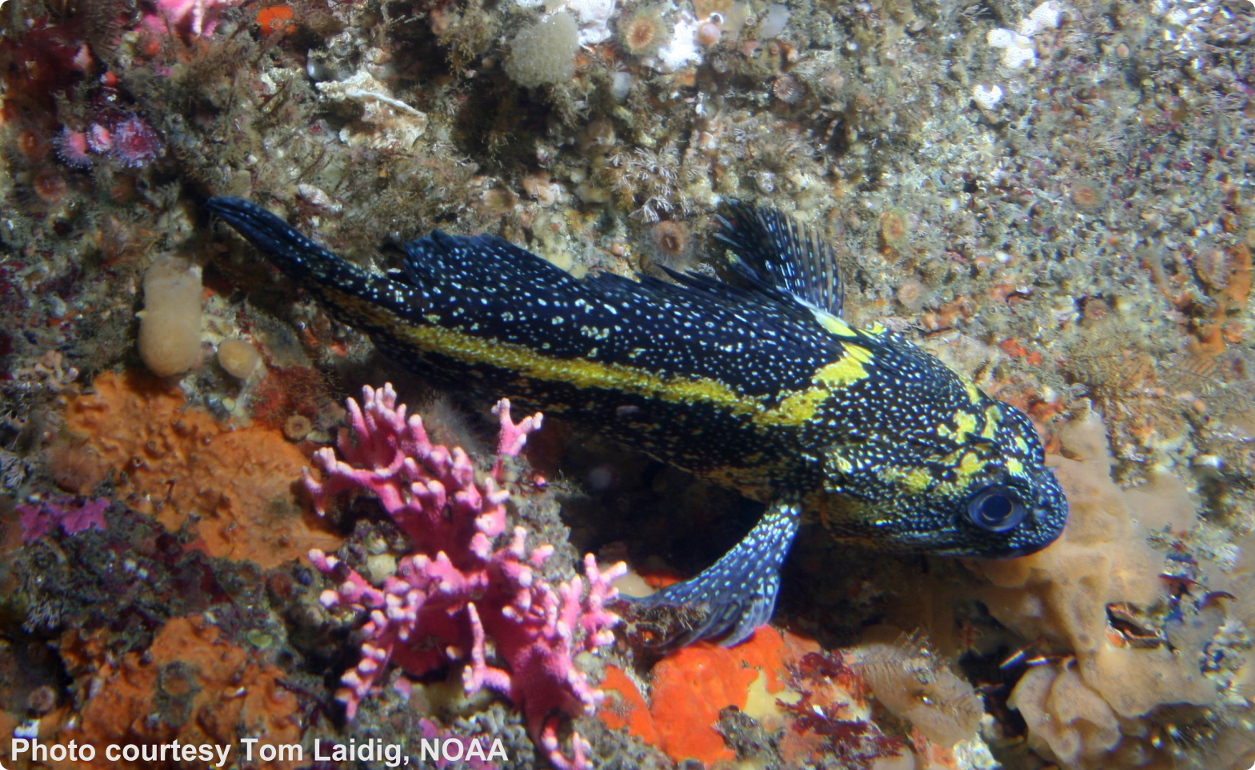
\includegraphics{cover_photo}~\\[1cm]
\pdftooltip{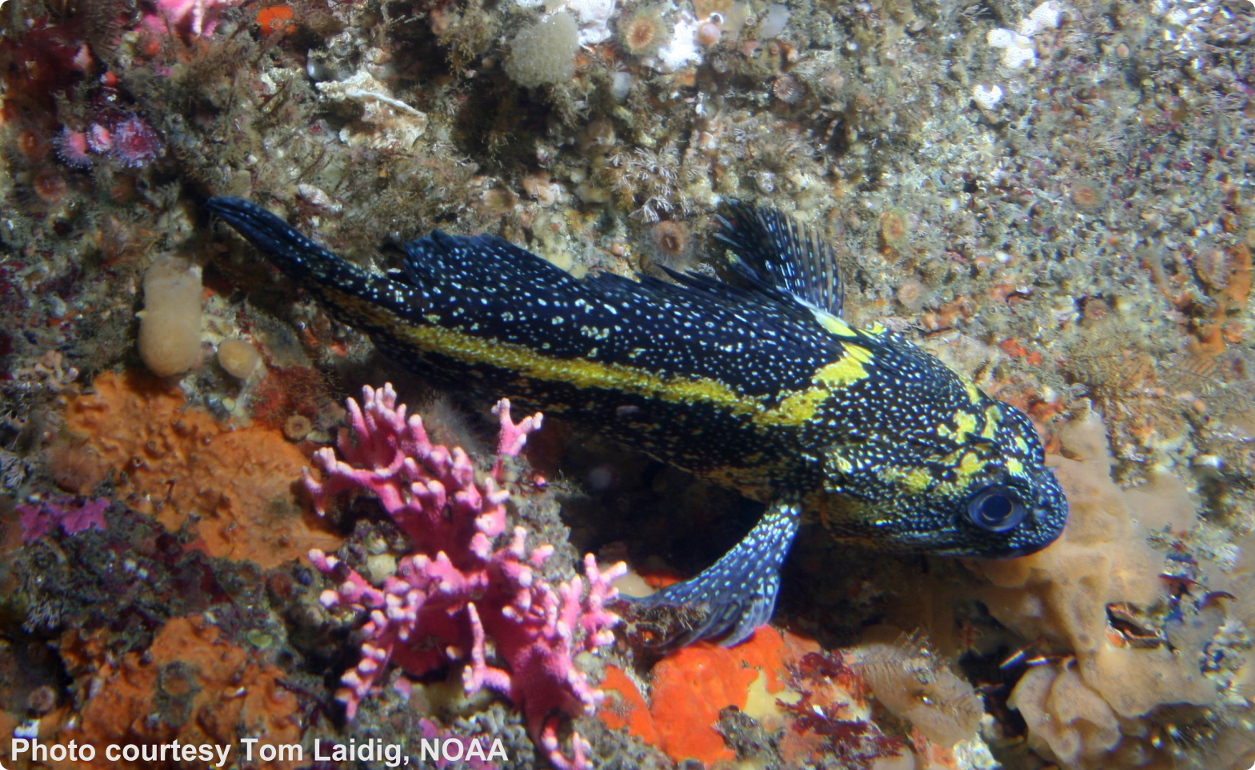
\includegraphics{cover_photo}}{This is a fish.}



Author No. 1\textsuperscript{1}\\
Author No. 2\textsuperscript{2}\\
Author No. 3\textsuperscript{3}\\

\vspace{.5cm}

\small
\textsuperscript{1}Southwest Fisheries Science Center, U.S. Department of Commerce, National Oceanic and Atmospheric Administration, National Marine Fisheries Service, 110 Shaffer Road, Santa Cruz, California 95060\\

\vspace{.3cm}

\textsuperscript{2}Northwest Fisheries Science Center, U.S. Department of Commerce, National Oceanic and Atmospheric Administration, National Marine Fisheries Service, 2725 Montlake Boulevard East, Seattle, Washington 98112\\

\vspace{.3cm}

\textsuperscript{3}Washington Department of Fish and Wildlife, 600 Capitol Way North, Olympia, Washington 98501\\


\vspace{.5cm}

\vfill
DRAFT SAFE\\
Disclaimer: This information is distributed solely for the purpose of pre-dissemination
peer review under applicable information quality guidelines. It has not been formally
disseminated by NOAA Fisheries. It does not represent and should not be construed to
represent any agency determination or policy. 

\vspace{.3cm}
%Bottom of the page
%{\large \today}


\newpage{\thispagestyle{empty}}


\begin{flushleft}
This report may be cited as:

ex. Monk, M. H. ,He, X., and Budrick, J. 2017. Status of the California Scorpionfish (\emph{Scorpaena guttata}) Off Southern California in 2017. Pacific Fishery Management Council, Portland, OR. Available from http://www.pcouncil.org/groundfish/stock-assessments/
\end{flushleft}

\maketitle

\pagenumbering{roman}
\setcounter{page}{1}
\end{center}

{
\setcounter{tocdepth}{4}
\tableofcontents
}
\setlength{\parskip}{5mm plus1mm minus1mm} \pagebreak

\setcounter{page}{1} \renewcommand{\thefigure}{\alph{figure}}
\renewcommand{\thetable}{\alph{table}}

\section*{Executive Summary}\label{executive-summary}
\addcontentsline{toc}{section}{Executive Summary}

\subsection*{Stock}\label{stock}
\addcontentsline{toc}{subsection}{Stock}

This assessment reports the status of the China rockfish
(\emph{Sebastes nebulosus}) resource in U.S. waters off the coast of
\ldots{} using data through 2014.

\subsection*{Catches}\label{catches}
\addcontentsline{toc}{subsection}{Catches}

Information on historical landings of China rockfish are available back
to xxxx\ldots{} (Table \ref{tab:Exec_catch}). Commercial landings were
small during the years of World War II, ranging between 0 to 0 metric
tons (mt) per year.

(Figures \ref{fig:Exec_catch1}-\ref{fig:Exec_catch2})\\
(Figure \ref{fig:r4ss_catches})

Since 2000, annual total landings of China rockfish have ranged between
2-4 mt, with landings in 2014 totaling 3 mt.

\FloatBarrier

\begin{figure}
\centering
\includegraphics{00_Assessment_Compile_files/figure-latex/unnamed-chunk-16-1.pdf}
\caption{China rockfish catch history for the recreational fleets.
\label{fig:Exec_catch1}}
\end{figure}

\begin{figure}
\centering
\includegraphics{00_Assessment_Compile_files/figure-latex/unnamed-chunk-17-1.pdf}
\caption{Stacked line plot of China rockfish catch history for the
commercial fleets. \label{fig:Exec_catch2}}
\end{figure}

\FloatBarrier

\begin{figure}
\centering
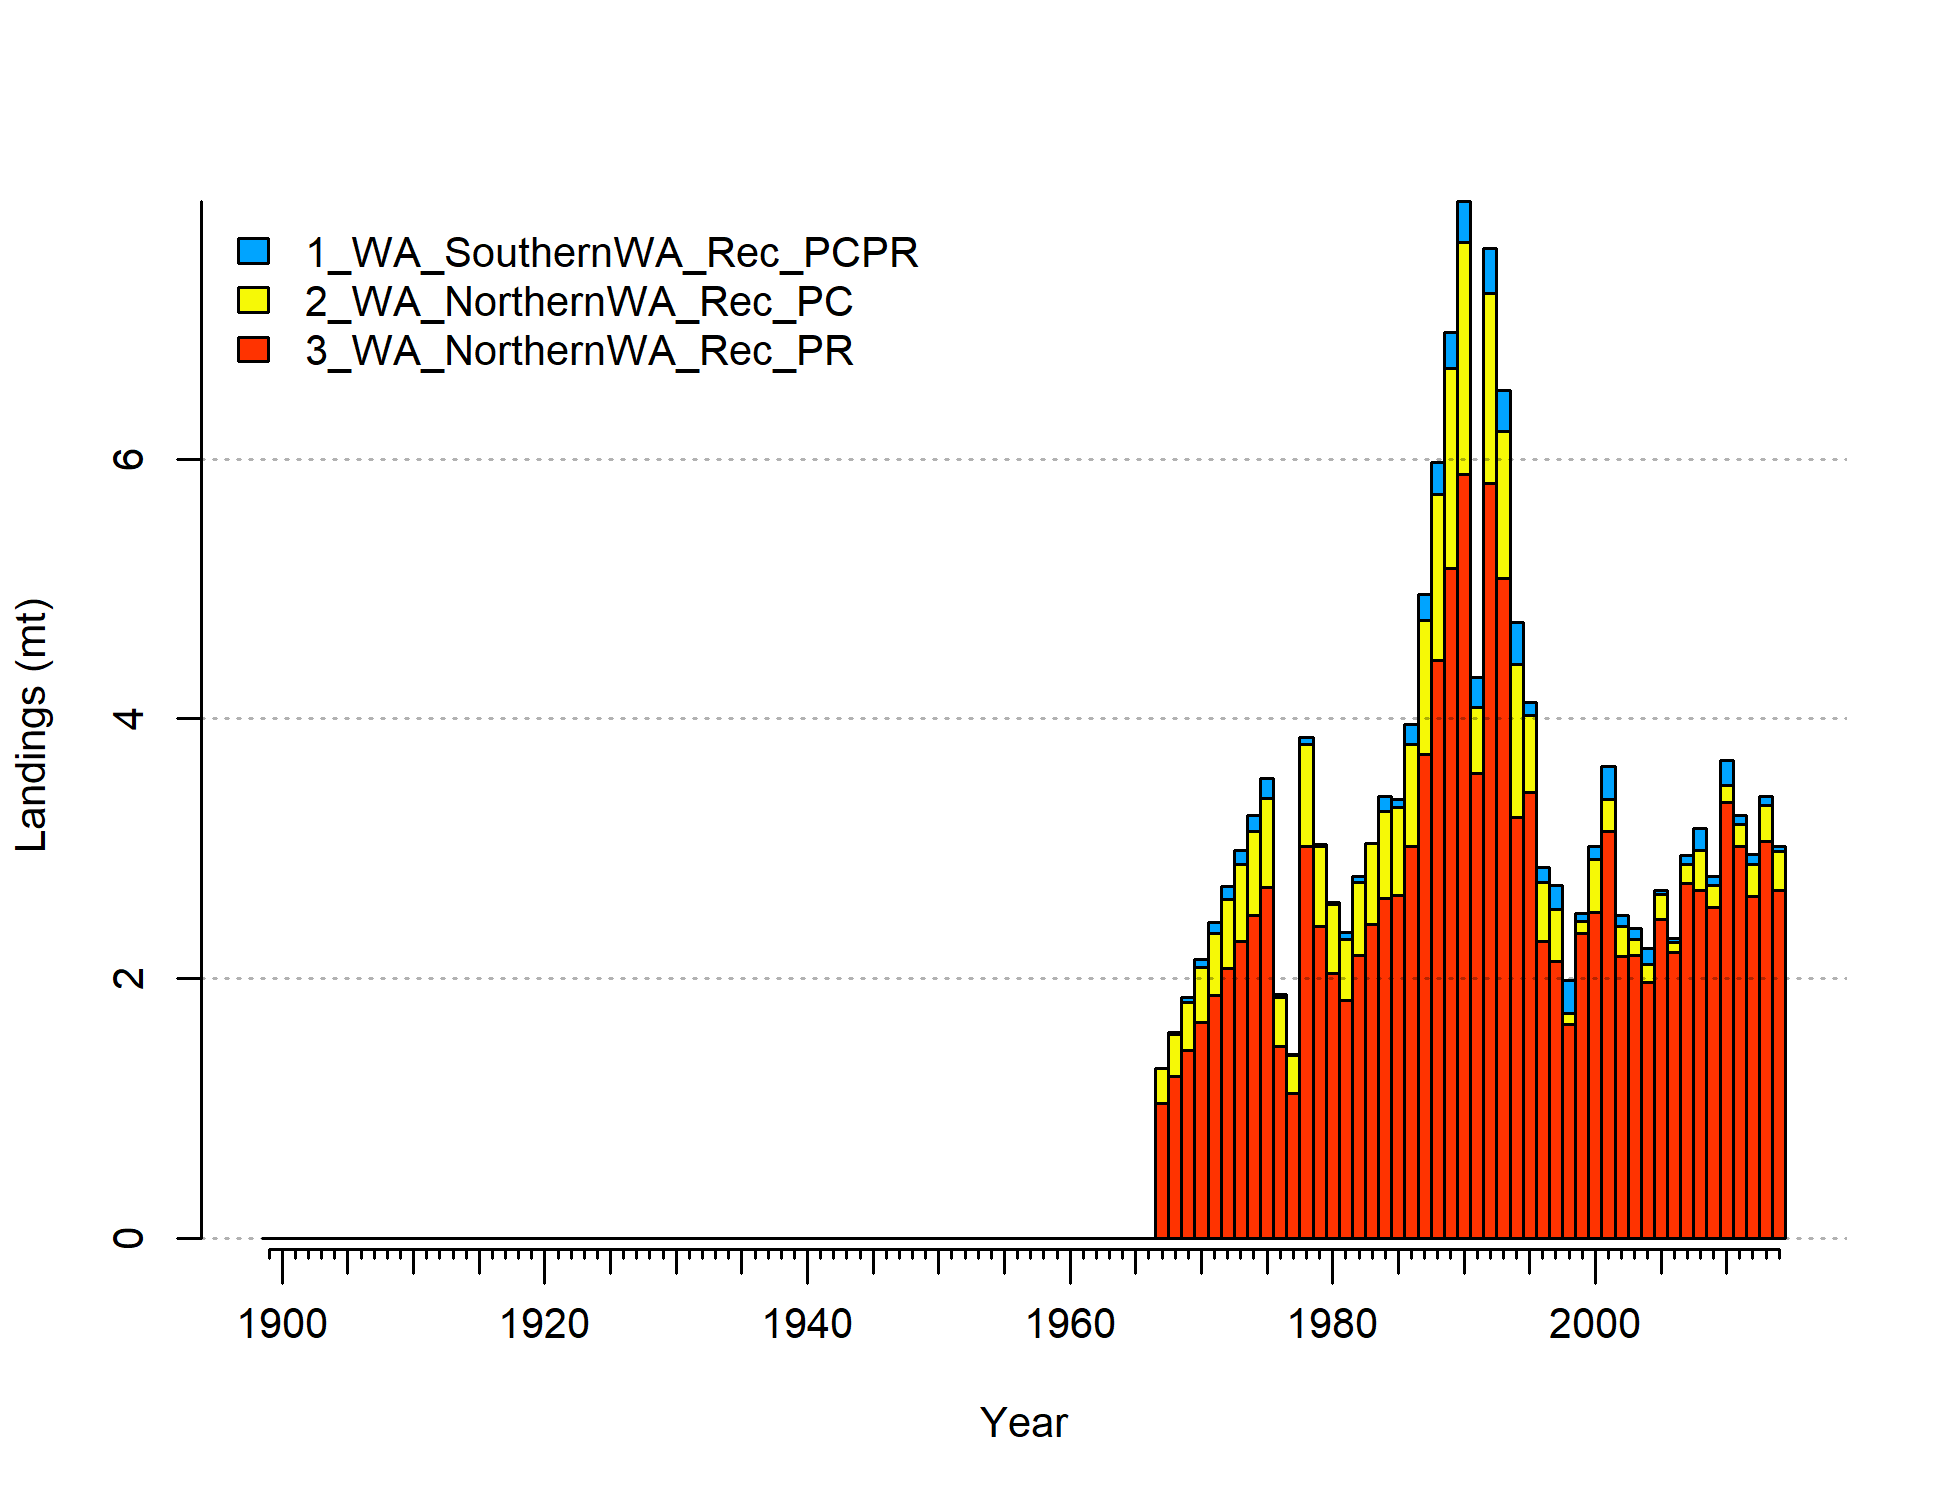
\includegraphics{r4ss/plots_mod1/catch2 landings stacked.png}
\caption{Catch history of China rockfish in the Northern model.
\label{fig:r4ss_catches}}
\end{figure}

\begin{table}[ht]
\centering
\caption{Recent China rockfish landings (mt) by 
                                            fleet.} 
\label{tab:Exec_catch}
\begin{tabular}{l>{\centering}p{1in}>{\centering}p{1in}>{\centering}p{1in}>{\centering}p{.9in}>{\centering}p{.9in}>{\centering}p{.6in}}
  \hline
Year & Landings 1 & Landings 2 & Landings 3 & Landings 4 & Landings 5 & Total \\ 
  \hline
2005 & - & - & - & - & - & - \\ 
  2006 & - & - & - & - & - & - \\ 
  2007 & - & - & - & - & - & - \\ 
  2008 & - & - & - & - & - & - \\ 
  2009 & - & - & - & - & - & - \\ 
  2010 & - & - & - & - & - & - \\ 
  2011 & - & - & - & - & - & - \\ 
  2012 & - & - & - & - & - & - \\ 
  2013 & - & - & - & - & - & - \\ 
  2014 & - & - & - & - & - & - \\ 
   \hline
\end{tabular}
\end{table}

\FloatBarrier

\newpage

\subsection*{Data and Assessment}\label{data-and-assessment}
\addcontentsline{toc}{subsection}{Data and Assessment}

This a new full assessment for China rockfish, which was last assessed
in \ldots{} using Stock Synthesis Version xx. This assessment uses the
newest version of Stock Synthesis (3.30.xx). The model begins in 1900,
and assumes the stock was at an unfished equilibrium that year.

(Figure \ref{fig:assess_region_map}).

\begin{figure}
\centering
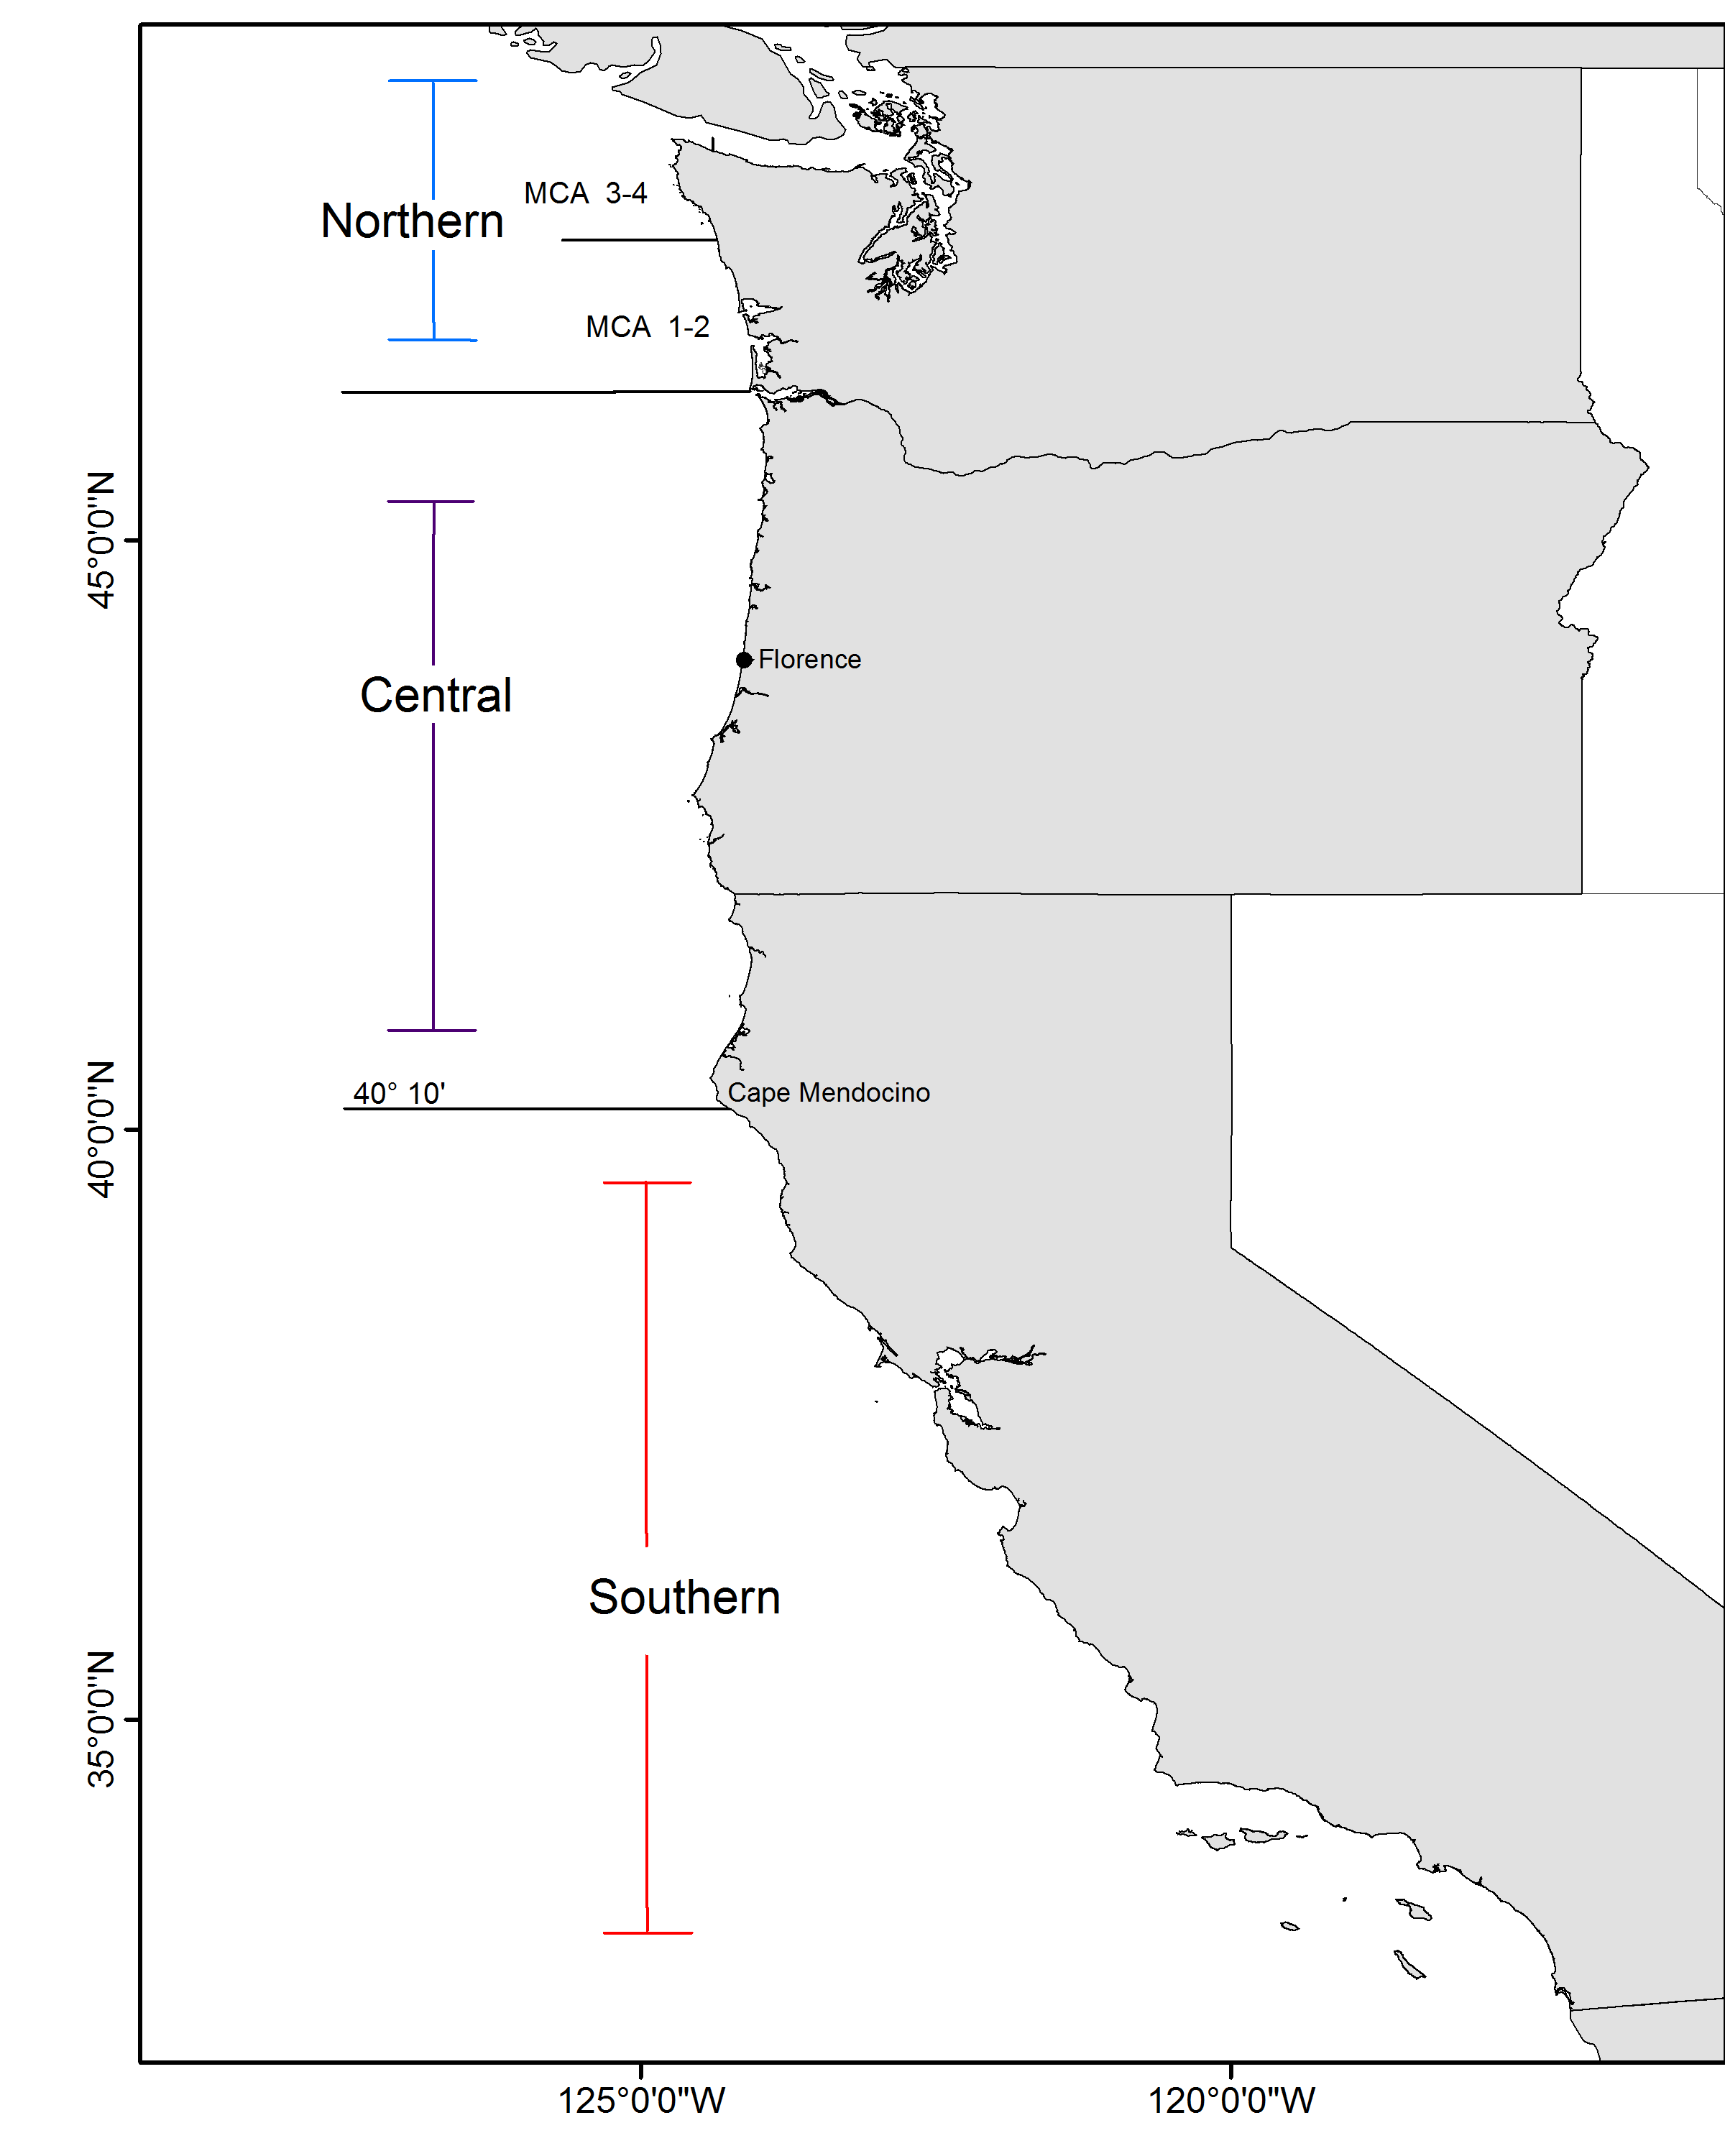
\includegraphics{Figures/assess_region_map.png}
\caption{Map depicting the distribution of California scorpionfish out
to 600 ft. The stock assessment is bounded at Pt. Conception in the
north to the U.S./Mexico border in the south.
\label{fig:assess_region_map}}
\end{figure}

\FloatBarrier

\subsection*{Stock Biomass}\label{stock-biomass}
\addcontentsline{toc}{subsection}{Stock Biomass}

(Figure \ref{fig:Spawnbio_all} and Table
\ref{tab:SpawningDeplete_mod1}).

The 2014 estimated spawning biomass relative to unfished equilibrium
spawning biomass is above the target of 40\% of unfished spawning
biomass at 73.4\% (95\% asymptotic interval: \(\pm\) 63.7\%-83.2\%)
(Figure \ref{fig:RelDeplete_all}). Approximate confidence intervals
based on the asymptotic variance estimates show that the uncertainty in
the estimated spawning biomass is high.

\FloatBarrier

\begin{table}[ht]
\centering
\caption{Recent trend in beginning of the 
                                      year spawning output and depletion for
                                      the Northern model for China rockfish.} 
\label{tab:SpawningDeplete_mod1}
\begin{tabular}{l>{\centering}p{1.3in}>{\centering}p{1.2in}>{\centering}p{1in}>{\centering}p{1.2in}}
  \hline
Year & Spawning Output (billion eggs) & \~{} 95\% confidence interval & Estimated depletion & \~{} 95\% confidence interval \\ 
  \hline
2006 & 17.942 & (8.86-27.03) & 0.734 & (0.638-0.83) \\ 
  2007 & 18.030 & (8.94-27.12) & 0.738 & (0.642-0.833) \\ 
  2008 & 18.044 & (8.95-27.14) & 0.738 & (0.643-0.833) \\ 
  2009 & 18.034 & (8.93-27.13) & 0.738 & (0.642-0.833) \\ 
  2010 & 18.062 & (8.96-27.17) & 0.739 & (0.644-0.834) \\ 
  2011 & 17.993 & (8.89-27.1) & 0.736 & (0.64-0.833) \\ 
  2012 & 17.971 & (8.86-27.08) & 0.735 & (0.638-0.832) \\ 
  2013 & 17.981 & (8.87-27.09) & 0.736 & (0.639-0.833) \\ 
  2014 & 17.944 & (8.83-27.06) & 0.734 & (0.637-0.832) \\ 
  2015 & 17.950 & (8.83-27.07) & 0.734 & (0.637-0.832) \\ 
   \hline
\end{tabular}
\end{table}

\FloatBarrier

\begin{figure}
\centering
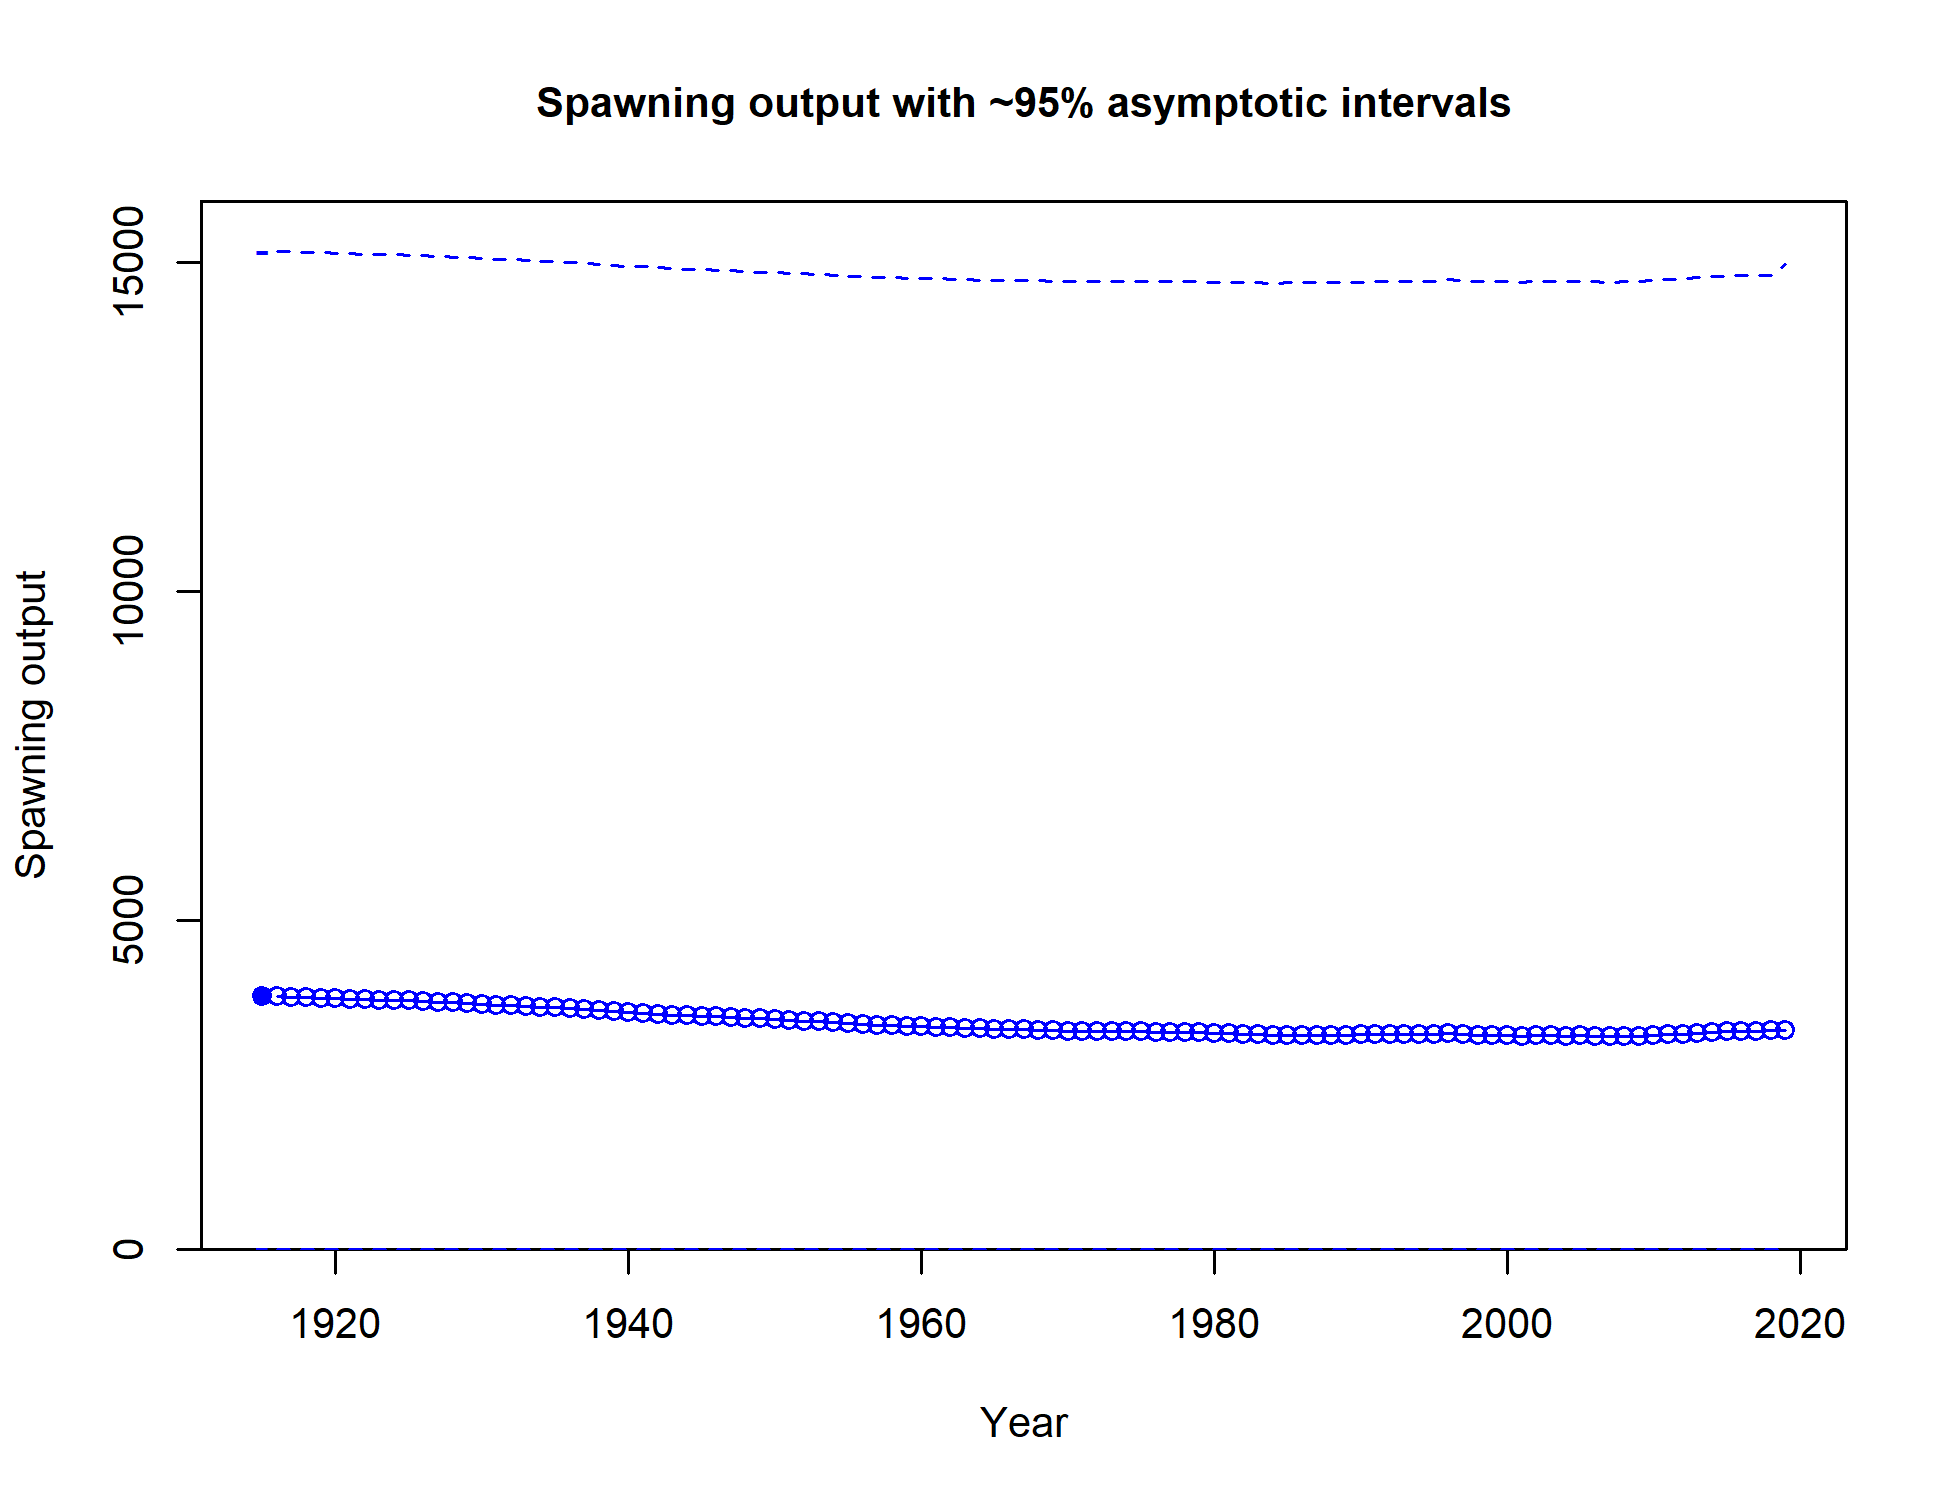
\includegraphics{r4ss/plots_mod1/ts7_Spawning_output_with_95_asymptotic_intervals_intervals.png}
\caption{Time series of spawning biomass trajectory (circles and line:
median; light broken lines: 95\% credibility intervals) for the base
case assessment model. \label{fig:Spawnbio_all}}
\end{figure}

\begin{figure}
\centering
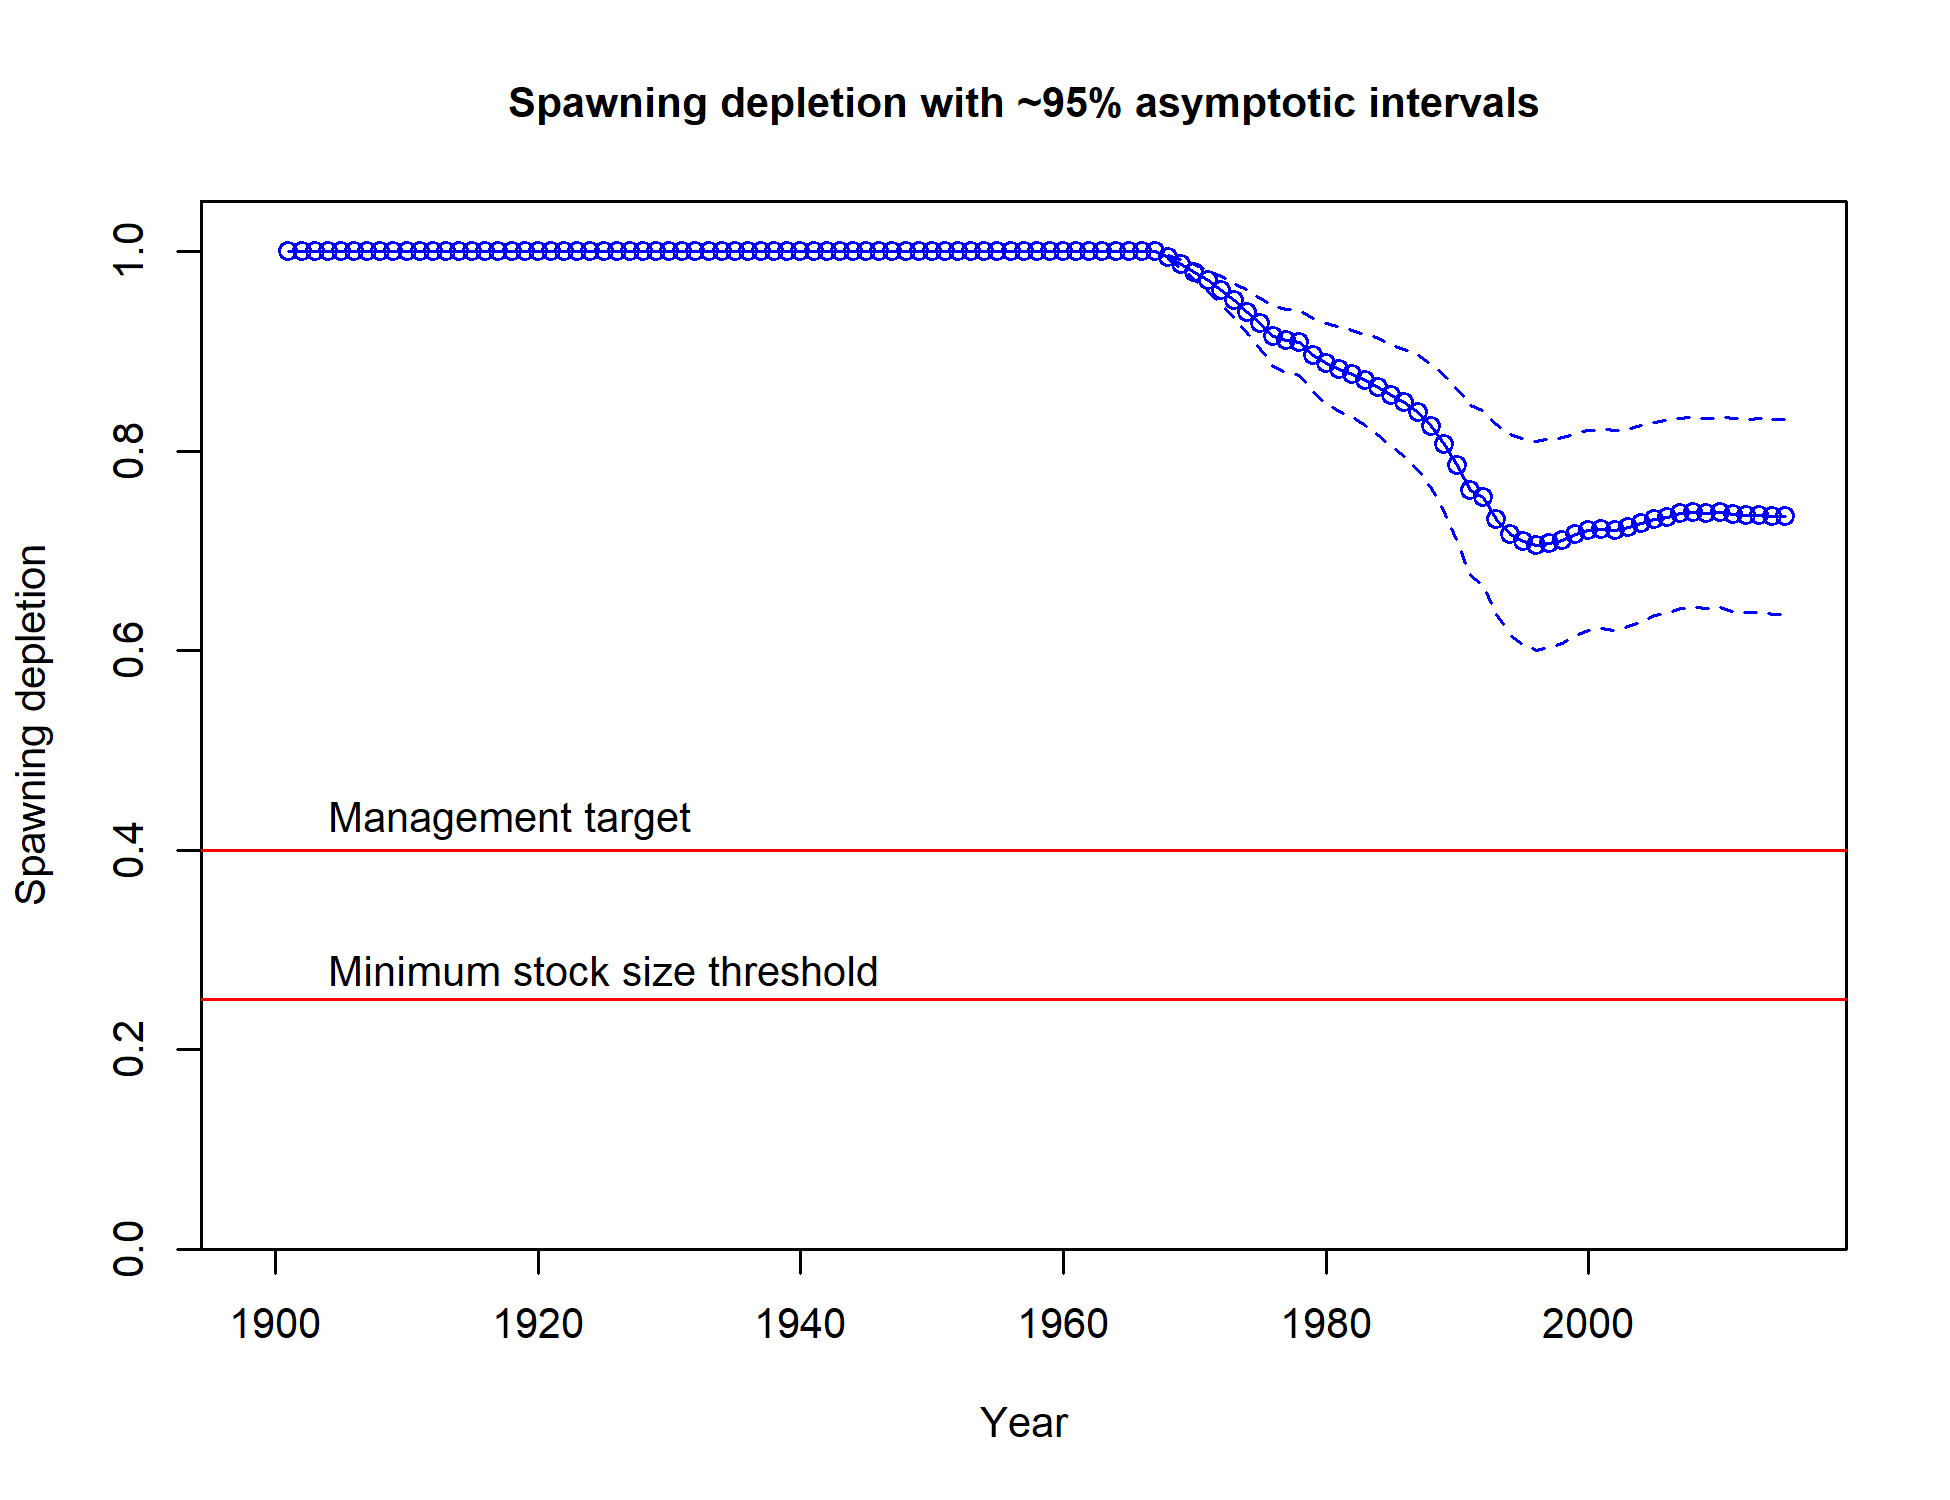
\includegraphics{r4ss/plots_mod1/ts9_Spawning_depletion_with_95_asymptotic_intervals_intervals.png}
\caption{Estimated relative depletion with approximate 95\% asymptotic
confidence intervals (dashed lines) for the base case assessment model.
\label{fig:RelDeplete_all}}
\end{figure}

\FloatBarrier

\subsection*{Recruitment}\label{recruitment}
\addcontentsline{toc}{subsection}{Recruitment}

Recruitment deviations were estimated from xxxx-xxxx (Figure
\ref{fig:Recruits_all} and Table \ref{tab:Recruit_mod1}).

\begin{table}[ht]
\centering
\caption{Recent recruitment for the Northern model.} 
\label{tab:Recruit_mod1}
\begin{tabular}{>{\centering}p{.8in}>{\centering}p{1.6in}>{\centering}p{1.3in}}
  \hline
Year & Estimated Recruitment (1,000s) & \~{} 95\% confidence interval \\ 
  \hline
2006 & 33.29 & (23.31 - 47.53) \\ 
  2007 & 33.30 & (23.33 - 47.54) \\ 
  2008 & 33.30 & (23.33 - 47.54) \\ 
  2009 & 33.30 & (23.33 - 47.54) \\ 
  2010 & 33.31 & (23.33 - 47.55) \\ 
  2011 & 33.30 & (23.32 - 47.54) \\ 
  2012 & 33.29 & (23.31 - 47.54) \\ 
  2013 & 33.29 & (23.32 - 47.54) \\ 
  2014 & 33.29 & (23.31 - 47.54) \\ 
  2015 & 33.29 & (23.31 - 47.54) \\ 
   \hline
\end{tabular}
\end{table}

\FloatBarrier

\begin{figure}
\centering
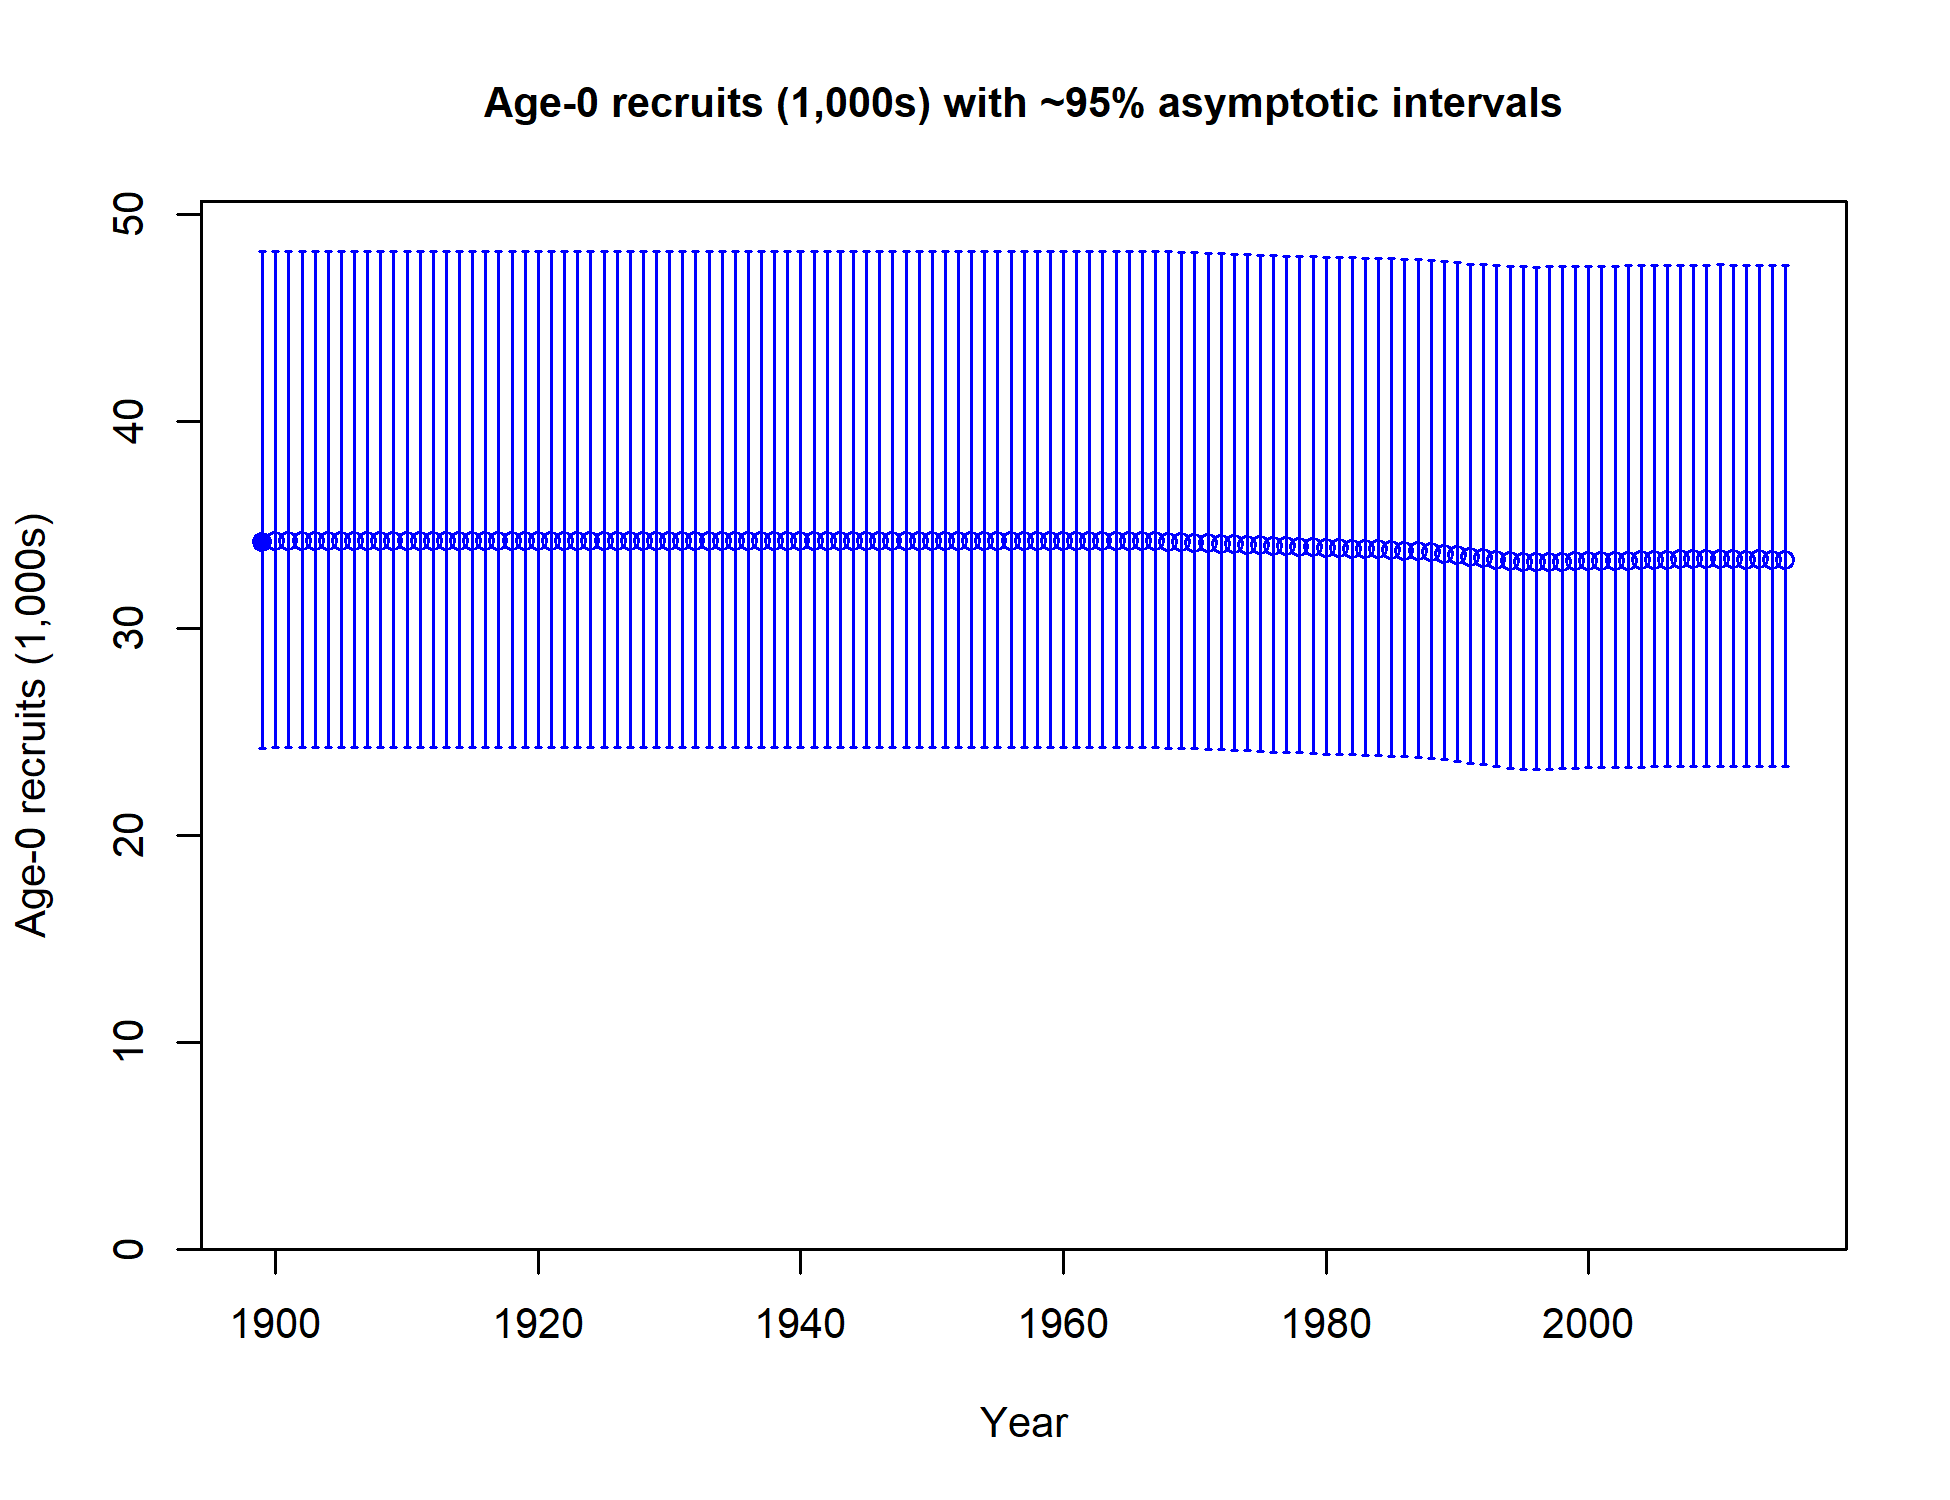
\includegraphics{r4ss/plots_mod1/ts11_Age-0_recruits_(1000s)_with_95_asymptotic_intervals.png}
\caption{Time series of estimated China rockfish recruitments for the
base-case model with 95\% confidence or credibility intervals.
\label{fig:Recruits_all}}
\end{figure}

\FloatBarrier

\subsection*{Exploitation status}\label{exploitation-status}
\addcontentsline{toc}{subsection}{Exploitation status}

Harvest rates estimated by the base model \ldots{}.. management target
levels (Table \ref{tab:SPR_Exploit_mod1} and Figure \ref{fig:SPR_all}).

\FloatBarrier

\begin{table}[ht]
\centering
\caption{Recent trend in spawning potential 
                                        ratio and exploitation for China rockfish in the Northern model.  Fishing intensity is (1-SPR) 
                                        divided by 50\% (the SPR target) and exploitation 
                                        is F divided by F\textsubscript{SPR}.} 
\label{tab:SPR_Exploit_mod1}
\begin{tabular}{l>{\centering}p{1in}>{\centering}p{1.2in}>{\centering}p{1in}>{\centering}p{1.2in}}
  \hline
Year & Fishing intensity & \~{} 95\% confidence interval & Exploitation rate & \~{} 95\% confidence interval \\ 
  \hline
2005 & 0.44 & (0.27-0.61) & 0.32 & (0.17-0.47) \\ 
  2006 & 0.39 & (0.24-0.55) & 0.28 & (0.15-0.4) \\ 
  2007 & 0.47 & (0.3-0.65) & 0.35 & (0.19-0.51) \\ 
  2008 & 0.50 & (0.32-0.68) & 0.38 & (0.2-0.55) \\ 
  2009 & 0.45 & (0.28-0.63) & 0.33 & (0.18-0.49) \\ 
  2010 & 0.56 & (0.36-0.76) & 0.44 & (0.24-0.64) \\ 
  2011 & 0.51 & (0.32-0.7) & 0.39 & (0.21-0.57) \\ 
  2012 & 0.48 & (0.3-0.66) & 0.35 & (0.19-0.52) \\ 
  2013 & 0.53 & (0.34-0.72) & 0.41 & (0.22-0.59) \\ 
  2014 & 0.48 & (0.3-0.67) & 0.36 & (0.19-0.53) \\ 
   \hline
\end{tabular}
\end{table}

\FloatBarrier

\begin{figure}
\centering
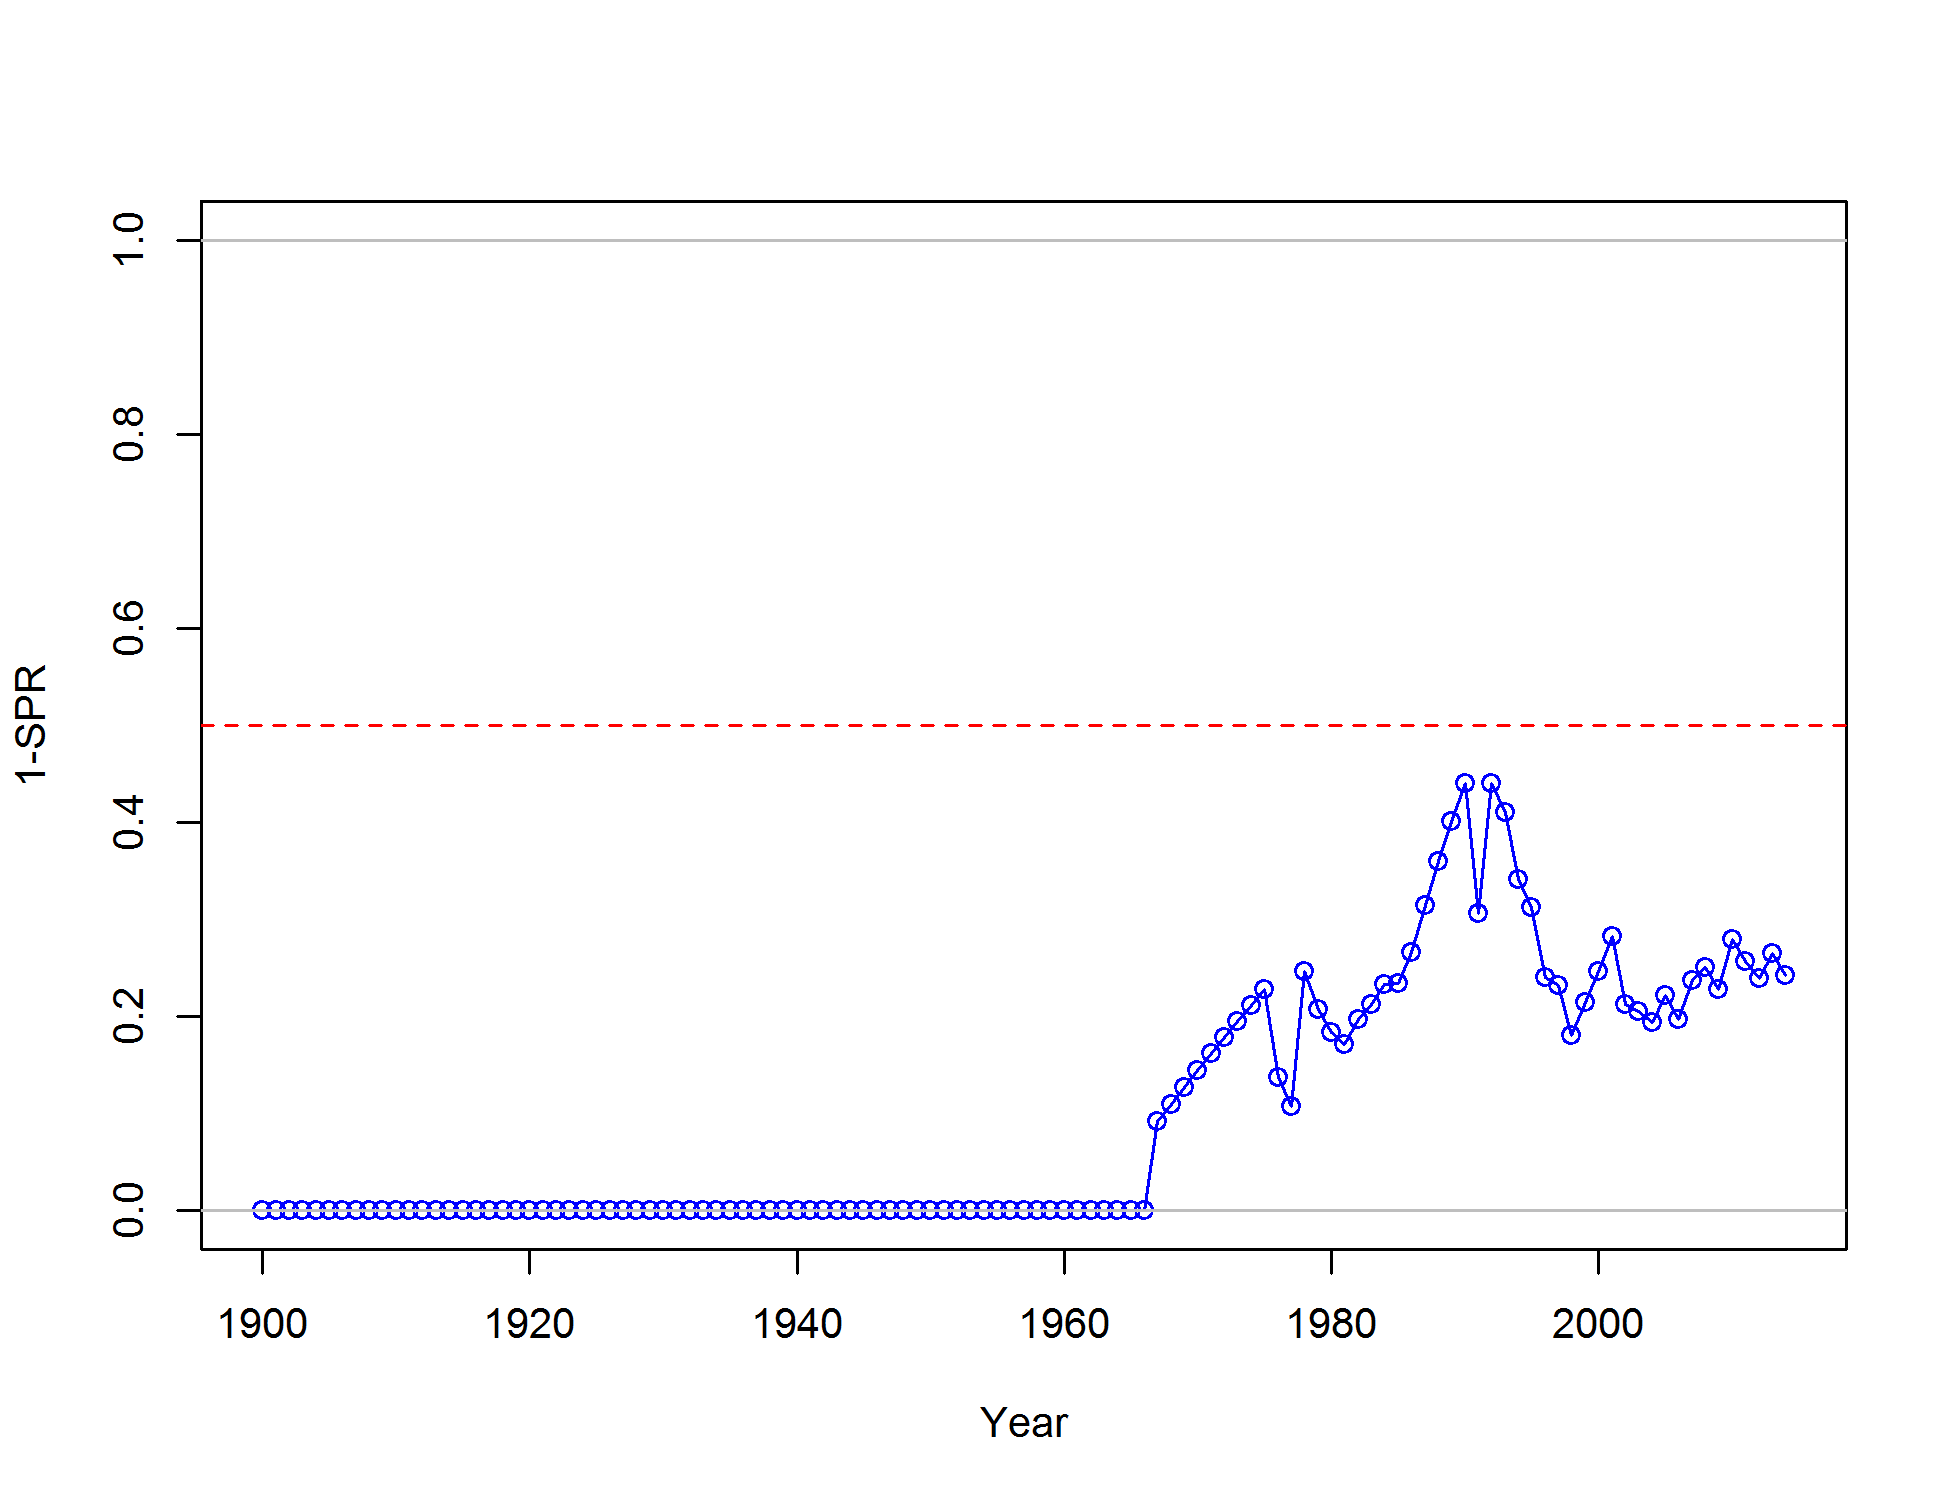
\includegraphics{r4ss/plots_mod1/SPR2_minusSPRseries.png}
\caption{Estimated spawning potential ratio (SPR) for the base-case
model. One minus SPR is plotted so that higher exploitation rates occur
on the upper portion of the y-axis. The management target is plotted as
a red horizontal line and values above this reflect harvests in excess
of the overfishing proxy based on the SPR\textsubscript{50\%} harvest
rate. The last year in the time series is 2014. \label{fig:SPR_all}}
\end{figure}

\FloatBarrier

\subsection*{Ecosystem Considerations}\label{ecosystem-considerations}
\addcontentsline{toc}{subsection}{Ecosystem Considerations}

In this assessment, ecosystem considerations were not explicitly
included in the analysis.\\
This is primarily due to a lack of relevant data and results of analyses
(conducted elsewhere) that could contribute ecosystem-related
quantitative information for the assessment.

\subsection*{Reference Points}\label{reference-points}
\addcontentsline{toc}{subsection}{Reference Points}

This stock assessment estimates that China rockfish in the Northern
model is above the biomass target (\(SB_{40\%}\)), and well above the
minimum stock size threshold (\(SB_{25\%}\)). The estimated relative
depletion level for the base model in 2015 is 73.4\% (95\% asymptotic
interval: \(\pm\) 63.7\%-83.2\%, corresponding to an unfished spawning
biomass of 17.9497 billion eggs (95\% asymptotic interval: 8.83-27.07
billion eggs) of spawning biomass in the base model (Table
\ref{tab:Ref_pts_mod1}). Unfished age 1+ biomass was estimated to be
240.8 mt in the base case model. The target spawning biomass
(\(SB_{40\%}\)) is 9.8 billion eggs, which corresponds with an
equilibrium yield of 6.3 mt. Equilibrium yield at the proxy \(F_{MSY}\)
harvest rate corresponding to \(SPR_{50\%}\) is 5.8 mt (Figure
\ref{fig:Yield_all}).

\FloatBarrier

\begin{table}[ht]
\centering
\caption{Summary of reference 
                                      points and management quantities for the 
                                      base case Northern model.} 
\label{tab:Ref_pts_mod1}
\begin{tabular}{>{\raggedright}p{4.1in}>{\centering}p{.65in}>{\centering}p{1.4in}}
  \hline
\textbf{Quantity} & \textbf{Estimate} & \textbf{\~95\%  Confidence Interval} \\ 
  \hline
Unfished spawning output (billion eggs) & 24.4 & (15.2-33.7) \\ 
  Unfished age 1+ biomass (mt) & 240.8 & (153-328.7) \\ 
  Unfished recruitment (R0, thousands) & 34.2 & (22.3-46) \\ 
  Spawning output(2014 billion eggs) & 17.9 & (8.8-27.1) \\ 
  Depletion (2014) & 0.7342 & (0.6367-0.8317) \\ 
  \textbf{$\text{Reference points based on } \mathbf{SB_{40\%}}$} &  &  \\ 
  Proxy spawning output ($B_{40\%}$) & 9.8 & (6.1-13.5) \\ 
  SPR resulting in $B_{40\%}$ ($SPR_{B40\%}$) & 0.444 & (0.444-0.444) \\ 
  Exploitation rate resulting in $B_{40\%}$ & 0.0551 & (0.0522-0.058) \\ 
  Yield with $SPR_{B40\%}$ at $B_{40\%}$ (mt) & 6.3 & (4-8.5) \\ 
  \textbf{\textit{Reference points based on SPR proxy for MSY}} &  &  \\ 
  Spawning output & 11.3 & (7-15.5) \\ 
  $SPR_{proxy}$ & 0.5 &  \\ 
  Exploitation rate corresponding to $SPR_{proxy}$ & 0.0458 & (0.0435-0.0482) \\ 
  Yield with $SPR_{proxy}$ at $SB_{SPR}$ (mt) & 5.8 & (3.7-7.9) \\ 
  \textbf{\textit{Reference points based on estimated MSY values}} &  &  \\ 
  Spawning output at $MSY$ ($SB_{MSY}$) & 5.6 & (3.5-7.8) \\ 
  $SPR_{MSY}$ & 0.2875 & (0.2823-0.2927) \\ 
  Exploitation rate at $MSY$ & 0.0924 & (0.0863-0.0985) \\ 
  $MSY$ (mt)  & 7 & (4.5-9.4) \\ 
   \hline
\end{tabular}
\end{table}

\FloatBarrier

\subsection*{Management Performance}\label{management-performance}
\addcontentsline{toc}{subsection}{Management Performance}

Table \ref{tab:mnmgt_perform}

\begin{table}[ht]
\centering
\caption{Recent trend in total catch and commercial 
                              landings (mt) relative to the management guidelines. 
                              Estimated total catch reflect the commercial landings 
                              plus the model estimated discarded biomass.} 
\label{tab:mnmgt_perform}
\scalebox{0.9}{
\begin{tabular}{>{\raggedleft}p{1in}>{\centering}p{1in}>{\centering}p{1in}>{\centering}p{1in}>{\centering}p{1in}}
  \hline
Year & OFL (mt; ABC prior to 2011) & ABC (mt) & ACL (mt; OY prior to 2011) & Estimated total catch (mt) \\ 
  \hline
\textbf{2007} & - & - & - & - \\ 
  \textbf{2008} & - & - & - & - \\ 
  \textbf{2009} & - & - & - & - \\ 
  \textbf{2010} & - & - & - & - \\ 
  \textbf{2011} & - & - & - & - \\ 
  \textbf{2012} & - & - & - & - \\ 
  \textbf{2013} & - & - & - & - \\ 
  \textbf{2014} & - & - & - & - \\ 
  \textbf{2015} & - & - & - & - \\ 
  \textbf{2016} & - & - & - & - \\ 
  \textbf{2017} & - & - & - & - \\ 
  \textbf{2018} & - & - & - & - \\ 
   \hline
\end{tabular}
}
\end{table}

\subsection*{Unresolved Problems and Major
Uncertainties}\label{unresolved-problems-and-major-uncertainties}
\addcontentsline{toc}{subsection}{Unresolved Problems and Major
Uncertainties}

\FloatBarrier

\subsection*{Decision Table}\label{decision-table}
\addcontentsline{toc}{subsection}{Decision Table}

\begin{table}[ht]
\centering
\caption{Projections of potential OFL (mt) for 
                                        each model, using the base model forecast.} 
\label{tab:OFL_projection}
\begin{tabular}{lr}
  \hline
Year & OFL \\ 
  \hline
2015 & 9.51 \\ 
  2016 & 9.57 \\ 
  2017 & 9.63 \\ 
  2018 & 9.29 \\ 
  2019 & 8.98 \\ 
  2020 & 8.69 \\ 
  2021 & 8.43 \\ 
  2022 & 8.20 \\ 
  2023 & 7.99 \\ 
  2024 & 7.80 \\ 
  2025 & 7.64 \\ 
  2026 & 7.49 \\ 
   \hline
\end{tabular}
\end{table}\begin{table}[ht]
\centering
\caption{Summary of 10-year 
                                             projections beginning in 2016 
                                             for alternate states of nature based on 
                                             an axis of uncertainty for the Northern model.  Columns range over low, mid, and high
                                             states of nature, and rows range over different 
                                             assumptions of catch levels. An entry of "--" 
                                             indicates that the stock is driven to very low 
                                             abundance under the particular scenario.} 
\label{tab:Decision_table_mod1}
\scalebox{0.85}{
\begin{tabular}{l|cc|>{\centering}p{.7in}c|>{\centering}p{.7in}c|>{\centering}p{.7in}c}
   \multicolumn{3}{c}{}  &  \multicolumn{2}{c}{} 
                               & \multicolumn{2}{c}{\textbf{States of nature}} 
                               & \multicolumn{2}{c}{} \\
  \multicolumn{3}{c}{}  &  \multicolumn{2}{c}{Low M 0.05} 
                               & \multicolumn{2}{c}{Base M 0.07} 
                               &  \multicolumn{2}{c}{High M 0.09} \\
 \hline
 & Year & Catch & Spawning Output & Depletion & Spawning Output & Depletion & Spawning Output & Depletion \\ 
  \hline
 & 2019 & - & - & - & - & - & - & - \\ 
   & 2020 & - & - & - & - & - & - & - \\ 
   & 2021 & - & - & - & - & - & - & - \\ 
  40-10 Rule,  & 2022 & - & - & - & - & - & - & - \\ 
  Low M & 2023 & - & - & - & - & - & - & - \\ 
   & 2024 & - & - & - & - & - & - & - \\ 
   & 2025 & - & - & - & - & - & - & - \\ 
   & 2026 & - & - & - & - & - & - & - \\ 
   & 2027 & - & - & - & - & - & - & - \\ 
   & 2028 & - & - & - & - & - & - & - \\ 
   \hline
 & 2019 & - & - & - & - & - & - & - \\ 
   & 2020 & - & - & - & - & - & - & - \\ 
   & 2021 & - & - & - & - & - & - & - \\ 
  40-10 Rule & 2022 & - & - & - & - & - & - & - \\ 
   & 2023 & - & - & - & - & - & - & - \\ 
   & 2024 & - & - & - & - & - & - & - \\ 
   & 2025 & - & - & - & - & - & - & - \\ 
   & 2026 & - & - & - & - & - & - & - \\ 
   & 2027 & - & - & - & - & - & - & - \\ 
   & 2028 & - & - & - & - & - & - & - \\ 
   \hline
 & 2019 & - & - & - & - & - & - & - \\ 
   & 2020 & - & - & - & - & - & - & - \\ 
   & 2021 & - & - & - & - & - & - & - \\ 
  40-10 Rule, & 2022 & - & - & - & - & - & - & - \\ 
  High M & 2023 & - & - & - & - & - & - & - \\ 
   & 2024 & - & - & - & - & - & - & - \\ 
   & 2025 & - & - & - & - & - & - & - \\ 
   & 2026 & - & - & - & - & - & - & - \\ 
   & 2027 & - & - & - & - & - & - & - \\ 
   & 2028 & - & - & - & - & - & - & - \\ 
   \hline
 & 2019 & - & - & - & - & - & - & - \\ 
   & 2020 & - & - & - & - & - & - & - \\ 
   & 2021 & - & - & - & - & - & - & - \\ 
  Average & 2022 & - & - & - & - & - & - & - \\ 
  Catch & 2023 & - & - & - & - & - & - & - \\ 
   & 2024 & - & - & - & - & - & - & - \\ 
   & 2025 & - & - & - & - & - & - & - \\ 
   & 2026 & - & - & - & - & - & - & - \\ 
   & 2027 & - & - & - & - & - & - & - \\ 
   & 2028 & - & - & - & - & - & - & - \\ 
   \hline
\end{tabular}
}
\end{table}

\begin{sidewaystable}[ht]
\centering
\caption{Base case results summary.} 
\label{tab:base_summary}
\scalebox{0.6}{
\begin{tabular}{r>{\centering}p{1.1in}>{\centering}p{1.1in}>{\centering}p{1.1in}>{\centering}p{1.1in}>{\centering}p{1.1in}>{\centering}p{1.1in}>{\centering}p{1.1in}>{\centering}p{1.1in}>{\centering}p{1.1in}>{\centering}p{1.1in}}
  \hline
Quantity & 2006 & 2007 & 2008 & 2009 & 2010 & 2011 & 2012 & 2013 & 2014 & 2015 \\ 
  \hline
Landings (mt) &  &  &  &  &  &  &  &  &  &  \\ 
  Total Est. Catch (mt) &  &  &  &  &  &  &  &  &  &  \\ 
  OFL (mt) &  &  &  &  &  &  &  &  &  &  \\ 
  ACL (mt) &  &  &  &  &  &  &  &  &  &  \\ 
   \hline
(1-$SPR$)(1-$SPR_{50\%}$) & 0.39 & 0.47 & 0.50 & 0.45 & 0.56 & 0.51 & 0.48 & 0.53 & 0.48 &  \\ 
   \hline
Exploitation rate & 0.28 & 0.35 & 0.38 & 0.33 & 0.44 & 0.39 & 0.35 & 0.41 & 0.36 &  \\ 
  Age 1+ biomass (mt) & 182.15 & 182.55 & 183.26 & 183.36 & 183.25 & 183.49 & 182.90 & 182.72 & 182.82 & 182.52 \\ 
   \hline
Spawning Output & 17.9 & 18.0 & 18.0 & 18.0 & 18.1 & 18.0 & 18.0 & 18.0 & 17.9 & 17.9 \\ 
  ~95\% CI & (8.86-27.03) & (8.94-27.12) & (8.95-27.14) & (8.93-27.13) & (8.96-27.17) & (8.89-27.1) & (8.86-27.08) & (8.87-27.09) & (8.83-27.06) & (8.83-27.07) \\ 
   \hline
Depletion & 0.7 & 0.7 & 0.7 & 0.7 & 0.7 & 0.7 & 0.7 & 0.7 & 0.7 & 0.7 \\ 
  ~95\% CI & (0.638-0.83) & (0.642-0.833) & (0.643-0.833) & (0.642-0.833) & (0.644-0.834) & (0.64-0.833) & (0.638-0.832) & (0.639-0.833) & (0.637-0.832) & (0.637-0.832) \\ 
   \hline
Recruits & 33.29 & 33.30 & 33.30 & 33.30 & 33.31 & 33.30 & 33.29 & 33.29 & 33.29 & 33.29 \\ 
  ~95\% CI & (23.31 - 47.53) & (23.33 - 47.54) & (23.33 - 47.54) & (23.33 - 47.54) & (23.33 - 47.55) & (23.32 - 47.54) & (23.31 - 47.54) & (23.32 - 47.54) & (23.31 - 47.54) & (23.31 - 47.54) \\ 
   \hline
\end{tabular}
}
\end{sidewaystable}

\begin{figure}
\centering
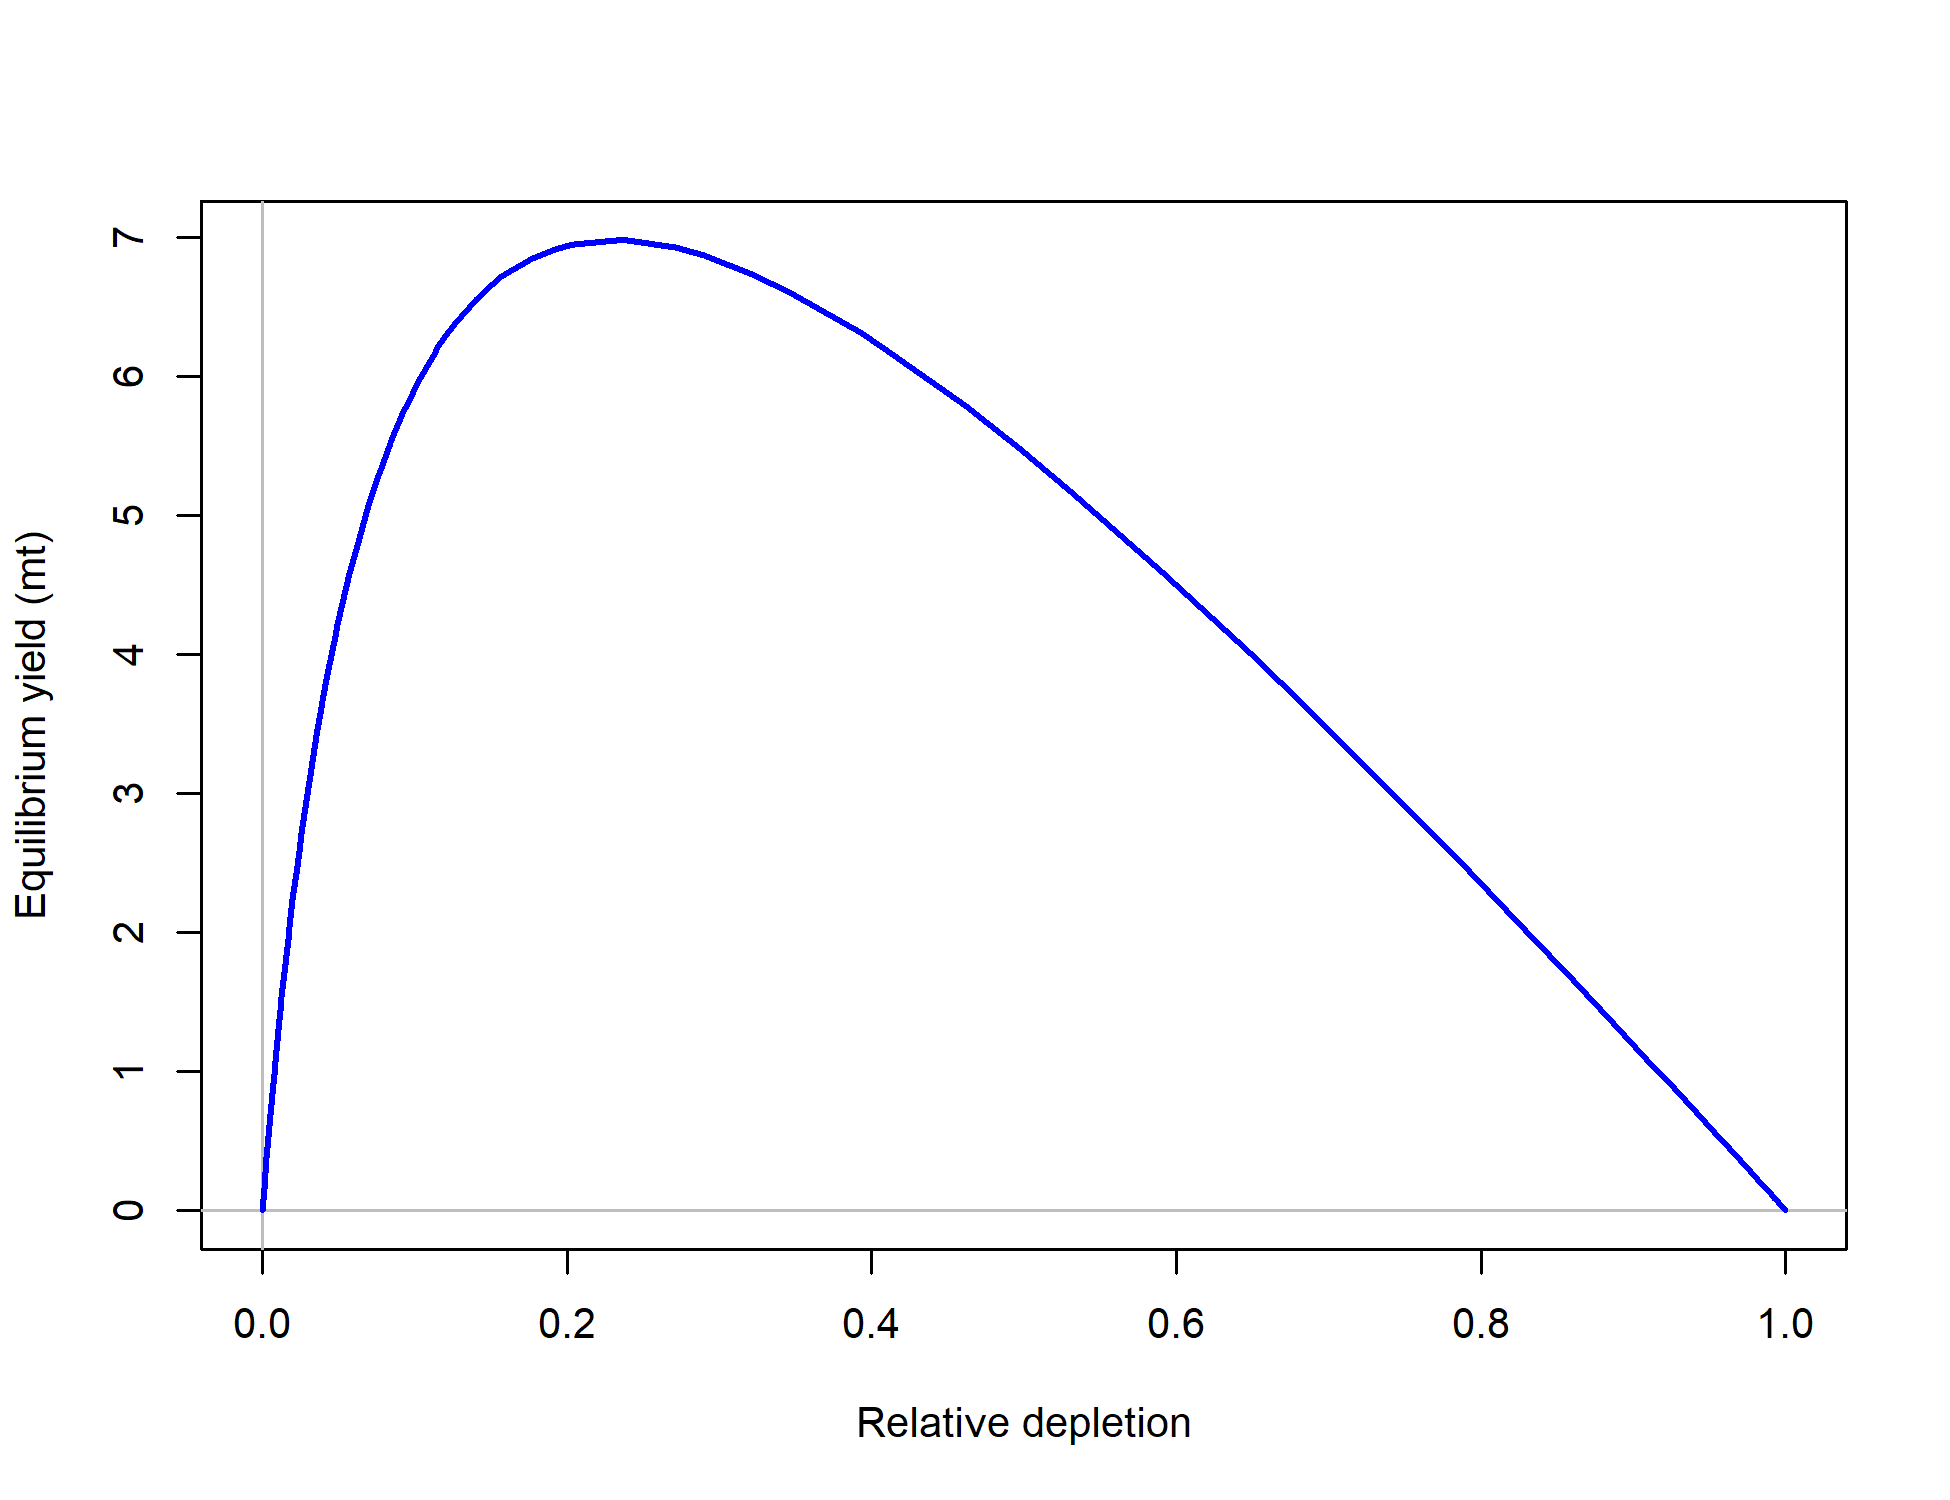
\includegraphics{r4ss/plots_mod1/yield1_yield_curve.png}
\caption{Equilibrium yield curve for the base case model. Values are
based on the 2014 fishery selectivity and with steepness fixed at 0.718.
\label{fig:Yield_all}}
\end{figure}

\FloatBarrier

\newpage

\subsection*{Research and Data Needs}\label{research-and-data-needs}
\addcontentsline{toc}{subsection}{Research and Data Needs}

We recommend the following research be conducted before the next
assessment:

\begin{enumerate}

\item \textbf{xxxx}: 

\item \textbf{xxxx}:

\item \textbf{xxxx}:

\item \textbf{xxxx}:

\item \textbf{xxxx}:

\end{enumerate}

\FloatBarrier

\newpage

\renewcommand{\thefigure}{\arabic{figure}}
\renewcommand{\thetable}{\arabic{table}}

\setcounter{figure}{0} \setcounter{table}{0}

\pagenumbering{arabic}

\section{Introduction}\label{introduction}

\subsection{Basic Information and Life
History}\label{basic-information-and-life-history}

\subsection{Early Life History}\label{early-life-history}

\subsection{Map}\label{map}

A map showing the scope of the assessment and depicting boundaries for
fisheries or data collection strata is provided in Figure
\ref{fig:boundary_map}.

\subsection{Ecosystem Considerations}\label{ecosystem-considerations-1}

In this assessment, ecosystem considerations were not explicitly
included in the analysis. This is primarily due to a lack of relevant
data and results of analyses (conducted elsewhere) that could contribute
ecosystem-related quantitative information for the assessment.

\subsection{Fishery Information}\label{fishery-information}

\subsection{Summary of Management
History}\label{summary-of-management-history}

\subsection{Management Performance}\label{management-performance-1}

Table \ref{tab:mnmgt_perform}

\subsection{Fisheries Off Mexico or
Canada}\label{fisheries-off-mexico-or-canada}

\section{Assessment}\label{assessment}

\subsection{Data}\label{data}

Data used in the China rockfish assessment are summarized in Figure
\ref{fig:data_plot}. Descriptions of the data sources are in the
following sections.

\subsubsection{Commercial Fishery
Landings}\label{commercial-fishery-landings}

\subsubsection{Commercial Discards}\label{commercial-discards}

\subsubsection{Commercial Fishery Length and Age
Data}\label{commercial-fishery-length-and-age-data}

The input sample sizes were calculated via the Stewart Method (Ian
Stewart, personal communication, IPHC):

\begin{centering}

Input effN = $N_{\text{trips}} + 0.138 * N_{\text{fish}}$ if $N_{\text{fish}}/N_{\text{trips}}$ is $<$ 44

Input effN = $7.06 * N_{\text{trips}}$ if $N_{\text{fish}}/N_{\text{trips}}$ is $\geq$ 44

\end{centering}

\subsubsection{Sport Fishery Removals and
Discards}\label{sport-fishery-removals-and-discards}

Biological samples from the recreational fleets are described in the
sections below.

\subsubsection{Fishery-Dependent Indices of
Abundance}\label{fishery-dependent-indices-of-abundance}

\textbf{Data Source 1}

\emph{Data Source 1 Index Standardization}

\emph{Data Source 1 Length Composition}

\textbf{Data Source 2}

\textbf{Data Source 3}

\subsubsection{Fishery-Independent Data
Sources}\label{fishery-independent-data-sources}

\textbf{Data Source 1}

\emph{Data Source 1 Index Standardization}

\emph{Data Source 1 Length Composition}

\textbf{Data Source 2}

\subsubsection{Biological Parameters and
Data}\label{biological-parameters-and-data}

Love et al. (\protect\hyperlink{ref-Love1987}{1987})

\textbf{Length and Age Compositions}

Length compositions were provided from the following sources:

\begin{itemize}[noitemsep,nolistsep,topsep=0pt]
  \item Source 1 (\emph{type, e.g., commercial dead fish, research, recreational}, yyyy-yyyy)    
  \item Source 2 (\emph{type}, yyyy-yyyy)    
  \item Source 3 (\emph{research}, yyyy, yyyy, yyyy, yyyy) 
\end{itemize}

The length composition of all fisheries aggregated across time by fleet
is in Figure \ref{fig:comp_lendat_aggregated_across_time}. Descriptions
and details of the length composition data are in the above section for
each fleet or survey.

\vspace{.5cm} \textbf{Age Structures}

von Bertalanffy growth curve (Bertalanffy
\protect\hyperlink{ref-vonB1938}{1938}),
\(L_i = L_{\infty}e^{(-k[t-t_0])}\), where \(L_i\) is the length (cm) at
age \(i\), \(t\) is age in years, \(k\) is rate of increase in growth,
\(t_0\) is the intercept, and \(L_{\infty}\) is the asymptotic length.

\vspace{.5cm} \textbf{Aging Precision and Bias}

\vspace{.5cm} \textbf{Weight-Length}

\vspace{.5cm} \textbf{Sex Ratio, Maturity, and Fecundity}

\vspace{.5cm} \textbf{Natural Mortality}

\vspace{.5cm}

\subsubsection{Environmental or Ecosystem Data Included in the
Assessment}\label{environmental-or-ecosystem-data-included-in-the-assessment}

In this assessment, neither environmental nor ecosystem considerations
were explicitly included in the analysis. This is primarily due to a
lack of relevant data and results of analyses (conducted elsewhere) that
could contribute ecosystem-related quantitative information for the
assessment.

\subsection{Previous Assessments}\label{previous-assessments}

\subsubsection{History of Modeling Approaches Used for this
Stock}\label{history-of-modeling-approaches-used-for-this-stock}

\subsubsection{yyyy Assessment
Recommendations}\label{yyyy-assessment-recommendations}

\begin{description}[style=unboxed]

  \item[Recommendation 1: ] \hfill \\

   STAT response: xxxxx

\item[Recommendation 2: ] \hfill \\

  STAT response: xxxxx

\item[Recommendation 3: ] \hfill \\

  STAT response: xxxx

  
\end{description}

\subsection{Model Description}\label{model-description}

\subsubsection{Transition to the Current Stock
Assessment}\label{transition-to-the-current-stock-assessment}

\subsubsection{Summary of Data for Fleets and
Areas}\label{summary-of-data-for-fleets-and-areas}

There are xxx fleets in the base model. They include:

\emph{Commercial}: The commercial fleets include \ldots{}

\emph{Recreational}: The recreational fleets include \ldots{}

\emph{Research}: There are xx sources of fishery-independent data
available \ldots{}

\subsubsection{Other Specifications}\label{other-specifications}

\subsubsection{Modeling Software}\label{modeling-software}

The STAT team used Stock Synthesis 3 version 3.30.05.03 by Dr.~Richard
Methot at the NWFSC. This most recent version was used, since it
included improvements and corrections to older versions. The r4SS
package (GitHub release number v1.27.0) was used to post-processing
output data from Stock Synthesis.

\subsubsection{Data Weighting}\label{data-weighting}

\subsubsection{Priors}\label{priors}

The log-normal prior for female natural mortality were based on a
meta-analysis completed by Hamel
(\protect\hyperlink{ref-Hamel2015}{2015}), as described under ``Natural
Mortality.'' Female natural mortality was fixed at the median of the
prior, 0.xxx for an assumed maximum age of xx. An uninformative prior
was used for the male offset natural mortality, which was estimated.

The prior for steepness (\emph{h}) assumes a beta distribution with
parameters based on an update for the Thorson-Dorn rockfish prior (Dorn,
M. and Thorson, J., pers. comm.), which was endorsed by the Science and
Statistical Committee in 2018. The prior is a beta distribution with
\(mu\)=0.xxx and \(sigma\)=0.xxx. Steepness is fixed in the base model
at the mean of the prior. The priors were applied in sensitivity
analyses where these parameters were estimated.

\subsubsection{Estimated and Fixed
Parameters}\label{estimated-and-fixed-parameters}

A full list of all estimated and fixed parameters is provided in Tables
\ref{tab:model_params}.

The base model has a total of xxx estimated parameters in the following
categories:

\begin{itemize}
  \item xxx,
  \item xxx
  \item xxx, and
  \item xxx selectivity parameters
\end{itemize}

The estimated parameters are described in greater detail below and a
full list of all estimated and parameters is provided in Table
\ref{tab:model_params}.

\emph{Growth.}

\emph{Natural Mortality.}

\emph{Selectivity.}

\emph{Other Estimated Parameters.}

\emph{Other Fixed Parameters.}

\subsection{Model Selection and
Evaluation}\label{model-selection-and-evaluation}

\subsubsection{Key Assumptions and Structural
Choices}\label{key-assumptions-and-structural-choices}

\subsubsection{Alternate Models
Considered}\label{alternate-models-considered}

\subsubsection{Convergence}\label{convergence}

\subsection{Response to the Current STAR Panel
Requests}\label{response-to-the-current-star-panel-requests}

\begin{description}[style=sameline]

\item[Request No. 1: ] \hfill \\
  
\textbf{Rationale:} xxx   
    
\textbf{STAT Response:} xxx


\item[Request No. 2: ] \hfill \\


\textbf{Rationale:} xxx 


\textbf{STAT Response:} xxx
    

\item[Request No. 3: ] \hfill \\

\textbf{Rationale:} x.  
    
  
\textbf{STAT Response:} xxx

\item[Request No. 4: ] \hfill \\

\textbf{Rationale:} xxx 
    
    
\textbf{STAT Response:} xxx


\item[Request No. 5: ] \hfill \\

\textbf{Rationale:} xxx
  
\textbf{STAT Response:} xxx  
    


\end{description}

\subsection{Base Case Model Results}\label{base-case-model-results}

The following description of the model results reflects a base model
that incorporates all of the changes made during the STAR panel (see
previous section). The base model parameter estimates and their
approximate asymptotic standard errors are shown in Table
\ref{tab:model_params} and the likelihood components are in Table
\ref{tab:like_components}. Estimates of derived reference points and
approximate 95\% asymptotic confidence intervals are shown in Table
\ref{tab:Ref_pts_mod1}. Time-series of estimated stock size over time
are shown in Table \ref{tab:Timeseries_mod1}.

\subsubsection{Parameter Estimates}\label{parameter-estimates}

The additional survey variability (process error added directly to each
year's input variability) for all surveys was estimated within the
model.

(Figure
\ref{fig:ts11_Age-0_recruits_(1000s)_with_95_asymptotic_intervals} ).

The stock-recruit curve \ldots{} Figure \ref{fig:SR_curve2} with
estimated recruitments also shown.

\subsubsection{Fits to the Data}\label{fits-to-the-data}

Model fits to the indices of abundance, fishery length composition,
survey length composition, and conditional age-at-length observations
are all discussed below.

\subsubsection{Uncertainty and Sensitivity
Analyses}\label{uncertainty-and-sensitivity-analyses}

A number of sensitivity analyses were conducted, including:

\begin{enumerate}

  \item Sensitivity 1
  
  \item Sensitivity 2
  
  \item Sensitivity 3
  
  \item Sensitivity 4
  
  \item Sensitivity 5, etc/
  
  
\end{enumerate}

\subsubsection{Retrospective Analysis}\label{retrospective-analysis}

\subsubsection{Likelihood Profiles}\label{likelihood-profiles}

\subsubsection{Reference Points}\label{reference-points-1}

Reference points were calculated using the estimated selectivities and
catch distribution among fleets in the most recent year of the model,
(2013). Sustainable total yield (landings plus discards) were 5.8 mt
when using an \(SPR_{50\%}\) reference harvest rate and with a 95\%
confidence interval of (3.7-7.9) mt based on estimates of uncertainty.
The spawning biomass equivalent to 40\% of the unfished level
(\(SB_{40\%}\)) was 9.8 mt.

(Figure
\ref{fig:ts7_Spawning_biomass_(mt)_with_95_asymptotic_intervals_intervals}

The 2014 spawning biomass relative to unfished equilibrium spawning
biomass is above/below the target of 40\% of unfished levels (Figure
\ref{fig:ts9_Spawning_depletion_with_95_asymptotic_intervals_intervals}).
The relative fishing intensity, \((1-SPR)/(1-SPR_{50\%})\), has been xxx
the management target for the entire time series of the model.

Table \ref{tab:Ref_pts_mod1} shows the full suite of estimated reference
points for the base model and Figure \ref{fig:yield1_yield_curve} shows
the equilibrium curve based on a steepness value xxx.

\section{Harvest Projections and Decision
Tables}\label{harvest-projections-and-decision-tables}

The forecasts of stock abundance and yield were developed using the
final base model, with the forecasted projections of the OFL presented
in Table \ref{tab:OFL_projection}.

The forecasted projections of the OFL for each model are presented in
Table \ref{tab:Decision_table_mod1}.

\section{Regional Management
Considerations}\label{regional-management-considerations}

\section{Research Needs}\label{research-needs}

There are a number of areas of research that could improve the stock
assessment for China rockfish. Below are issues identified by the STAT
team and the STAR panel:

\begin{enumerate}

\item \textbf{xxxx}: 

\item \textbf{xxxx}:

\item \textbf{xxxx}:

\item \textbf{xxxx}:

\item \textbf{xxxx}:

\end{enumerate}

\section{Acknowledgments}\label{acknowledgments}

\newpage

\FloatBarrier

\section{Tables}\label{tables}

\FloatBarrier

\FloatBarrier

\FloatBarrier
\newpage

\newpage

\FloatBarrier
<!-- ********************************************************************** -->

\FloatBarrier
<!-- ********************************************************************** -->

\FloatBarrier
<!-- ********************************************************************** -->

\FloatBarrier
<!-- ********************************************************************** -->

\FloatBarrier

\begin{table}[ht]
\centering
\caption{Results from 100 jitters from the base 
                                      case model.} 
\label{tab:jitter}
\begin{tabular}{llll}
  \hline
Description & Value & NA & NA \\ 
  \hline
Returned to base case & - & - & - \\ 
  Found local minimum & - & - & - \\ 
  Found better solution & - & - & - \\ 
  Error in likelihood & - & - & - \\ 
  Total & 100 & 100 & 100 \\ 
   \hline
\end{tabular}
\end{table}

\begin{landscape}
\begin{longtable}{rlrrcccl}
\caption{List of parameters used in
                                              the base model, including estimated 
                                              values and standard deviations (SD), 
                                              bounds (minimum and maximum), 
                                              estimation phase (negative values indicate
                                              not estimated), status (indicates if 
                                              parameters are near bounds, and prior type
                                              information (mean, SD).} \\ 
  \hline
No. & Parameter & Value & Phase & Bounds & Status & SD & Prior (Exp.Val, SD)  \\ 
  \hline 
\endhead 
\hline 
\multicolumn{3}{l}{\footnotesize Continued on next page} 
\endfoot 
\endlastfoot 
 \hline
1 & NatM\_p\_1\_Fem\_GP\_1 & 0.070 & -3 & (0.01, 0.15) &  &  & Log\_Norm (-2.94, 0.53) \\ 
  2 & L\_at\_Amin\_Fem\_GP\_1 & 2.000 & -2 & (-10, 45) &  &  & Normal (2, 10) \\ 
  3 & L\_at\_Amax\_Fem\_GP\_1 & 35.411 & 6 & (20, 50) & OK & 0.364 & Normal (34, 10) \\ 
  4 & VonBert\_K\_Fem\_GP\_1 & 0.147 & 6 & (0.01, 0.3) & OK & 0.006 & Normal (0.1, 0.8) \\ 
  5 & CV\_young\_Fem\_GP\_1 & 0.100 & -6 & (0.01, 0.25) &  &  & None \\ 
  6 & CV\_old\_Fem\_GP\_1 & 0.080 & 6 & (0.01, 0.25) & OK & 0.007 & None \\ 
  7 & NatM\_p\_1\_Mal\_GP\_1 & 0.000 & -3 & (-1, 0.15) &  &  & None \\ 
  8 & L\_at\_Amin\_Mal\_GP\_1 & 0.000 & -2 & (-1, 45) &  &  & Normal (2, 10) \\ 
  9 & L\_at\_Amax\_Mal\_GP\_1 & 0.000 & -4 & (-1, 50) &  &  & Normal (33.13, 10) \\ 
  10 & VonBert\_K\_Mal\_GP\_1 & 0.000 & -4 & (-1, 0.3) &  &  & Normal (0.2461, 0.8) \\ 
  11 & CV\_young\_Mal\_GP\_1 & 0.000 & -3 & (-1, 0.25) &  &  & None \\ 
  12 & CV\_old\_Mal\_GP\_1 & 0.000 & -3 & (-1, 0.25) &  &  & None \\ 
  13 & Wtlen\_1\_Fem & 0.000 & -3 & (0, 1) &  &  & None \\ 
  14 & Wtlen\_2\_Fem & 3.177 & -3 & (2, 4) &  &  & None \\ 
  15 & Mat50\%\_Fem & 28.500 & -3 & (1, 100) &  &  & None \\ 
  16 & Mat\_slope\_Fem & -1.000 & -3 & (-9, 9) &  &  & None \\ 
  17 & Eggs/kg\_inter\_Fem & 0.196 & -3 & (-3, 3) &  &  & None \\ 
  18 & Eggs/kg\_slope\_wt\_Fem & 0.057 & -3 & (-3, 3) &  &  & None \\ 
  19 & Wtlen\_1\_Mal & 0.000 & -3 & (0, 1) &  &  & None \\ 
  20 & Wtlen\_2\_Mal & 3.177 & -3 & (2, 4) &  &  & None \\ 
  24 & CohortGrowDev & 0.000 & -4 & (0, 0) &  &  & None \\ 
  25 & SR\_LN(R0) & 3.531 & 1 & (2, 12) & OK & 0.177 & None \\ 
  26 & SR\_BH\_steep & 0.773 & -3 & (0.2, 1) &  &  & Full\_Beta (0.773, 0.147) \\ 
  27 & SR\_sigmaR & 0.500 & -3 & (0, 2) &  &  & None \\ 
  28 & SR\_envlink & 0.100 & -3 & (-5, 5) &  &  & None \\ 
  29 & SR\_R1\_offset & 0.000 & -4 & (-5, 5) &  &  & None \\ 
  30 & SR\_autocorr & 0.000 & -99 & (0, 0) &  &  & None \\ 
  68 & InitF\_11\_WA\_SouthernWA\_Rec\_PCPR & 0.000 & -1 & (0, 1) &  &  & None \\ 
  69 & InitF\_22\_WA\_NorthernWA\_Rec\_PC & 0.000 & -1 & (0, 1) &  &  & None \\ 
  70 & InitF\_33\_WA\_NorthernWA\_Rec\_PR & 0.000 & -1 & (0, 1) &  &  & None \\ 
  71 & Q\_extraSD\_3\_3\_WA\_NorthernWA\_Rec\_PR & 0.126 & 2 & (0, 2) & OK & 0.024 & None \\ 
  72 & SizeSel\_1P\_1\_1\_WA\_SouthernWA\_Rec\_PCPR & 34.890 & -4 & (19, 36) &  &  & None \\ 
  73 & SizeSel\_1P\_2\_1\_WA\_SouthernWA\_Rec\_PCPR & -4.000 & -9 & (-9, 5) &  &  & None \\ 
  74 & SizeSel\_1P\_3\_1\_WA\_SouthernWA\_Rec\_PCPR & 3.970 & 5 & (0, 9) & OK & 0.364 & None \\ 
  75 & SizeSel\_1P\_4\_1\_WA\_SouthernWA\_Rec\_PCPR & 8.000 & -9 & (0, 9) &  &  & None \\ 
  76 & SizeSel\_1P\_5\_1\_WA\_SouthernWA\_Rec\_PCPR & -8.000 & -9 & (-9, 9) &  &  & None \\ 
  77 & SizeSel\_1P\_6\_1\_WA\_SouthernWA\_Rec\_PCPR & 8.000 & -9 & (-9, 9) &  &  & None \\ 
  78 & SizeSel\_2P\_1\_2\_WA\_NorthernWA\_Rec\_PC & 34.862 & 4 & (19, 36) & OK & 1.001 & None \\ 
  79 & SizeSel\_2P\_2\_2\_WA\_NorthernWA\_Rec\_PC & -4.000 & -9 & (-9, 5) &  &  & None \\ 
  80 & SizeSel\_2P\_3\_2\_WA\_NorthernWA\_Rec\_PC & 2.925 & 5 & (0, 9) & OK & 0.347 & None \\ 
  81 & SizeSel\_2P\_4\_2\_WA\_NorthernWA\_Rec\_PC & 8.000 & -9 & (0, 9) &  &  & None \\ 
  82 & SizeSel\_2P\_5\_2\_WA\_NorthernWA\_Rec\_PC & -8.000 & -9 & (-9, 9) &  &  & None \\ 
  83 & SizeSel\_2P\_6\_2\_WA\_NorthernWA\_Rec\_PC & 8.000 & -9 & (-9, 9) &  &  & None \\ 
   \hline
\hline
\label{tab:model_params}
\end{longtable}
\end{landscape}

\FloatBarrier

\begin{table}[ht]
\centering
\caption{Likelihood components from the base model.} 
\label{tab:like_components}
\begin{tabular}{lr}
  \hline
Likelihood component & Value \\ 
  \hline
TOTAL & 1097.30 \\ 
  Catch & 0.00 \\ 
  Survey & -98.12 \\ 
  Length composition & 763.02 \\ 
  Age composition & 421.52 \\ 
  Recruitment & 10.88 \\ 
  Forecast recruitment & 0.00 \\ 
  Parameter priors & 0.00 \\ 
  Parmeter soft bounds & 0.01 \\ 
   \hline
\end{tabular}
\end{table}

\newpage

\begin{longtable}{c>{\centering}p{.6in}>{\centering}p{.6in}>{\centering}p{.6in}>{\centering}p{.6in}>{\centering}p{.8in}>{\centering}p{.8in}c}
\caption{Time-series of population estimates 
                                        from the base-case model. Relative exploitation 
                                        rate is $(1-SPR)/(1-SPR_{50\%})$.} \\ 
  \hline
Year & Total biomass (mt) & Spawning biomass (mt) & Depletion & Age-0 recruits & Total catch (mt) & Relative exploitation rate & SPR \\ 
  \hline  \endfirsthead \caption[]{Time-series of population estimates 
                                        from the base-case model. Relative exploitation 
                                        rate is $(1-SPR)/(1-SPR_{50\%})$.} \label{tab:Timeseries_mod1} \\ \hline Year & Total biomass (mt) & Spawning biomass (mt) & Depletion & Age-0 recruits & Total catch (mt) & Relative exploitation rate & SPR \\ \hline  \endhead \hline \multicolumn{5}{l}{\textit{Continues next page}} \ 
                                 \endfoot
                                 \endlastfoot \hline
1900 & 241 & 24 & 0.000 & 34 & 0 & 0.00 & 1.00 \\ 
  1901 & 241 & 24 & 0.000 & 34 & 0 & 0.00 & 1.00 \\ 
  1902 & 241 & 24 & 0.000 & 34 & 0 & 0.00 & 1.00 \\ 
  1903 & 241 & 24 & 0.000 & 34 & 0 & 0.00 & 1.00 \\ 
  1904 & 241 & 24 & 0.000 & 34 & 0 & 0.00 & 1.00 \\ 
  1905 & 241 & 24 & 0.000 & 34 & 0 & 0.00 & 1.00 \\ 
  1906 & 241 & 24 & 0.000 & 34 & 0 & 0.00 & 1.00 \\ 
  1907 & 241 & 24 & 0.000 & 34 & 0 & 0.00 & 1.00 \\ 
  1908 & 241 & 24 & 0.000 & 34 & 0 & 0.00 & 1.00 \\ 
  1909 & 241 & 24 & 0.000 & 34 & 0 & 0.00 & 1.00 \\ 
  1910 & 241 & 24 & 0.000 & 34 & 0 & 0.00 & 1.00 \\ 
  1911 & 241 & 24 & 0.000 & 34 & 0 & 0.00 & 1.00 \\ 
  1912 & 241 & 24 & 0.000 & 34 & 0 & 0.00 & 1.00 \\ 
  1913 & 241 & 24 & 0.000 & 34 & 0 & 0.00 & 1.00 \\ 
  1914 & 241 & 24 & 0.000 & 34 & 0 & 0.00 & 1.00 \\ 
  1915 & 241 & 24 & 0.000 & 34 & 0 & 0.00 & 1.00 \\ 
  1916 & 241 & 24 & 0.000 & 34 & 0 & 0.00 & 1.00 \\ 
  1917 & 241 & 24 & 0.000 & 34 & 0 & 0.00 & 1.00 \\ 
  1918 & 241 & 24 & 0.000 & 34 & 0 & 0.00 & 1.00 \\ 
  1919 & 241 & 24 & 0.000 & 34 & 0 & 0.00 & 1.00 \\ 
  1920 & 241 & 24 & 0.000 & 34 & 0 & 0.00 & 1.00 \\ 
  1921 & 241 & 24 & 0.000 & 34 & 0 & 0.00 & 1.00 \\ 
  1922 & 241 & 24 & 0.000 & 34 & 0 & 0.00 & 1.00 \\ 
  1923 & 241 & 24 & 0.000 & 34 & 0 & 0.00 & 1.00 \\ 
  1924 & 241 & 24 & 0.000 & 34 & 0 & 0.00 & 1.00 \\ 
  1925 & 241 & 24 & 0.000 & 34 & 0 & 0.00 & 1.00 \\ 
  1926 & 241 & 24 & 0.000 & 34 & 0 & 0.00 & 1.00 \\ 
  1927 & 241 & 24 & 0.000 & 34 & 0 & 0.00 & 1.00 \\ 
  1928 & 241 & 24 & 0.000 & 34 & 0 & 0.00 & 1.00 \\ 
  1929 & 241 & 24 & 0.000 & 34 & 0 & 0.00 & 1.00 \\ 
  1930 & 241 & 24 & 0.000 & 34 & 0 & 0.00 & 1.00 \\ 
  1931 & 241 & 24 & 0.000 & 34 & 0 & 0.00 & 1.00 \\ 
  1932 & 241 & 24 & 0.000 & 34 & 0 & 0.00 & 1.00 \\ 
  1933 & 241 & 24 & 0.000 & 34 & 0 & 0.00 & 1.00 \\ 
  1934 & 241 & 24 & 0.000 & 34 & 0 & 0.00 & 1.00 \\ 
  1935 & 241 & 24 & 0.000 & 34 & 0 & 0.00 & 1.00 \\ 
  1936 & 241 & 24 & 0.000 & 34 & 0 & 0.00 & 1.00 \\ 
  1937 & 241 & 24 & 0.000 & 34 & 0 & 0.00 & 1.00 \\ 
  1938 & 241 & 24 & 0.000 & 34 & 0 & 0.00 & 1.00 \\ 
  1939 & 241 & 24 & 0.000 & 34 & 0 & 0.00 & 1.00 \\ 
  1940 & 241 & 24 & 0.000 & 34 & 0 & 0.00 & 1.00 \\ 
  1941 & 241 & 24 & 0.000 & 34 & 0 & 0.00 & 1.00 \\ 
  1942 & 241 & 24 & 0.000 & 34 & 0 & 0.00 & 1.00 \\ 
  1943 & 241 & 24 & 0.000 & 34 & 0 & 0.00 & 1.00 \\ 
  1944 & 241 & 24 & 0.000 & 34 & 0 & 0.00 & 1.00 \\ 
  1945 & 241 & 24 & 0.000 & 34 & 0 & 0.00 & 1.00 \\ 
  1946 & 241 & 24 & 0.000 & 34 & 0 & 0.00 & 1.00 \\ 
  1947 & 241 & 24 & 0.000 & 34 & 0 & 0.00 & 1.00 \\ 
  1948 & 241 & 24 & 0.000 & 34 & 0 & 0.00 & 1.00 \\ 
  1949 & 241 & 24 & 0.000 & 34 & 0 & 0.00 & 1.00 \\ 
  1950 & 241 & 24 & 0.000 & 34 & 0 & 0.00 & 1.00 \\ 
  1951 & 241 & 24 & 0.000 & 34 & 0 & 0.00 & 1.00 \\ 
  1952 & 241 & 24 & 0.000 & 34 & 0 & 0.00 & 1.00 \\ 
  1953 & 241 & 24 & 0.000 & 34 & 0 & 0.00 & 1.00 \\ 
  1954 & 241 & 24 & 0.000 & 34 & 0 & 0.00 & 1.00 \\ 
  1955 & 241 & 24 & 0.000 & 34 & 0 & 0.00 & 1.00 \\ 
  1956 & 241 & 24 & 0.000 & 34 & 0 & 0.00 & 1.00 \\ 
  1957 & 241 & 24 & 0.000 & 34 & 0 & 0.00 & 1.00 \\ 
  1958 & 241 & 24 & 0.000 & 34 & 0 & 0.00 & 1.00 \\ 
  1959 & 241 & 24 & 0.000 & 34 & 0 & 0.00 & 1.00 \\ 
  1960 & 241 & 24 & 0.000 & 34 & 0 & 0.00 & 1.00 \\ 
  1961 & 241 & 24 & 0.000 & 34 & 0 & 0.00 & 1.00 \\ 
  1962 & 241 & 24 & 0.000 & 34 & 0 & 0.00 & 1.00 \\ 
  1963 & 241 & 24 & 0.000 & 34 & 0 & 0.00 & 1.00 \\ 
  1964 & 241 & 24 & 0.000 & 34 & 0 & 0.00 & 1.00 \\ 
  1965 & 241 & 24 & 0.000 & 34 & 0 & 0.00 & 1.00 \\ 
  1966 & 241 & 24 & 0.000 & 34 & 0 & 0.00 & 1.00 \\ 
  1967 & 241 & 24 & 0.000 & 34 & 1 & 0.00 & 0.91 \\ 
  1968 & 240 & 24 & 0.994 & 34 & 2 & 0.00 & 0.89 \\ 
  1969 & 238 & 24 & 0.987 & 34 & 2 & 0.17 & 0.87 \\ 
  1970 & 237 & 24 & 0.980 & 34 & 2 & 0.20 & 0.86 \\ 
  1971 & 235 & 24 & 0.971 & 34 & 2 & 0.23 & 0.84 \\ 
  1972 & 233 & 23 & 0.961 & 34 & 3 & 0.26 & 0.82 \\ 
  1973 & 231 & 23 & 0.951 & 34 & 3 & 0.29 & 0.80 \\ 
  1974 & 229 & 23 & 0.940 & 34 & 3 & 0.32 & 0.79 \\ 
  1975 & 226 & 23 & 0.928 & 34 & 4 & 0.35 & 0.77 \\ 
  1976 & 224 & 22 & 0.915 & 34 & 2 & 0.19 & 0.86 \\ 
  1977 & 223 & 22 & 0.911 & 34 & 1 & 0.14 & 0.89 \\ 
  1978 & 223 & 22 & 0.909 & 34 & 4 & 0.39 & 0.75 \\ 
  1979 & 220 & 22 & 0.896 & 34 & 3 & 0.31 & 0.79 \\ 
  1980 & 219 & 22 & 0.888 & 34 & 3 & 0.27 & 0.82 \\ 
  1981 & 217 & 22 & 0.882 & 34 & 2 & 0.24 & 0.83 \\ 
  1982 & 217 & 21 & 0.878 & 34 & 3 & 0.29 & 0.80 \\ 
  1983 & 215 & 21 & 0.871 & 34 & 3 & 0.32 & 0.79 \\ 
  1984 & 214 & 21 & 0.864 & 34 & 3 & 0.36 & 0.77 \\ 
  1985 & 212 & 21 & 0.856 & 34 & 3 & 0.36 & 0.77 \\ 
  1986 & 211 & 21 & 0.849 & 34 & 4 & 0.42 & 0.73 \\ 
  1987 & 209 & 20 & 0.839 & 34 & 5 & 0.53 & 0.69 \\ 
  1988 & 206 & 20 & 0.825 & 34 & 6 & 0.65 & 0.64 \\ 
  1989 & 202 & 20 & 0.807 & 34 & 7 & 0.77 & 0.60 \\ 
  1990 & 198 & 19 & 0.786 & 33 & 8 & 0.90 & 0.56 \\ 
  1991 & 193 & 19 & 0.761 & 33 & 4 & 0.50 & 0.69 \\ 
  1992 & 192 & 18 & 0.753 & 33 & 8 & 0.89 & 0.56 \\ 
  1993 & 187 & 18 & 0.732 & 33 & 7 & 0.78 & 0.59 \\ 
  1994 & 184 & 18 & 0.716 & 33 & 5 & 0.58 & 0.66 \\ 
  1995 & 183 & 17 & 0.709 & 33 & 4 & 0.51 & 0.69 \\ 
  1996 & 182 & 17 & 0.705 & 33 & 3 & 0.35 & 0.76 \\ 
  1997 & 183 & 17 & 0.708 & 33 & 3 & 0.33 & 0.77 \\ 
  1998 & 183 & 17 & 0.711 & 33 & 2 & 0.24 & 0.82 \\ 
  1999 & 185 & 18 & 0.717 & 33 & 2 & 0.30 & 0.79 \\ 
  2000 & 185 & 18 & 0.720 & 33 & 3 & 0.37 & 0.75 \\ 
  2001 & 186 & 18 & 0.722 & 33 & 4 & 0.44 & 0.72 \\ 
  2002 & 185 & 18 & 0.720 & 33 & 2 & 0.30 & 0.79 \\ 
  2003 & 186 & 18 & 0.724 & 33 & 2 & 0.29 & 0.80 \\ 
  2004 & 187 & 18 & 0.728 & 33 & 2 & 0.27 & 0.81 \\ 
  2005 & 188 & 18 & 0.732 & 33 & 3 & 0.32 & 0.78 \\ 
  2006 & 188 & 18 & 0.734 & 33 & 2 & 0.28 & 0.80 \\ 
  2007 & 189 & 18 & 0.738 & 33 & 3 & 0.35 & 0.76 \\ 
  2008 & 189 & 18 & 0.738 & 33 & 3 & 0.38 & 0.75 \\ 
  2009 & 189 & 18 & 0.738 & 33 & 3 & 0.33 & 0.77 \\ 
  2010 & 189 & 18 & 0.739 & 33 & 4 & 0.44 & 0.72 \\ 
  2011 & 188 & 18 & 0.736 & 33 & 3 & 0.39 & 0.74 \\ 
  2012 & 188 & 18 & 0.735 & 33 & 3 & 0.35 & 0.76 \\ 
  2013 & 188 & 18 & 0.736 & 33 & 3 & 0.41 & 0.74 \\ 
  2014 & 188 & 18 & 0.734 & 33 & 3 & 0.36 & 0.76 \\ 
  2015 & 188 & 18 & 0.734 & 33 &  &  &  \\ 
   \hline
\hline
\end{longtable}

\FloatBarrier

\begin{sidewaystable}[ht]
\centering
\caption{Sensitivity of the base model 
                                          to dropping or down-weighting data 
                                          sources and alternative assumptions 
                                          about growth.} 
\label{tab:Sensitivity_model1}
\scalebox{0.9}{
\begin{tabular}{l>{\centering}p{.8in}>{\centering}p{.8in}>{\centering}p{.8in}>{\centering}p{.8in}>{\centering}p{.8in}>{\centering}p{.8in}>{\centering}p{.8in}>{\centering}p{.8in}}
  \hline
Label & Base (Francis weights) & Default weights & Harmonic mean weights & Estimate equal M & Estimate equal M and h & Drop PR data & Drop PC data & Drop RecDD data \\ 
  \hline
TOTAL\_like & - & - & - & - & - & - & - & - \\ 
  Catch\_like & - & - & - & - & - & - & - & - \\ 
  Equil\_catch\_like & - & - & - & - & - & - & - & - \\ 
  Survey\_like & - & - & - & - & - & - & - & - \\ 
  Length\_comp\_like & - & - & - & - & - & - & - & - \\ 
  Age\_comp\_like & - & - & - & - & - & - & - & - \\ 
  Parm\_priors\_like & - & - & - & - & - & - & - & - \\ 
  SSB\_Unfished\_thousand\_mt & - & - & - & - & - & - & - & - \\ 
  TotBio\_Unfished & - & - & - & - & - & - & - & - \\ 
  SmryBio\_Unfished & - & - & - & - & - & - & - & - \\ 
  Recr\_Unfished\_billions & - & - & - & - & - & - & - & - \\ 
  SSB\_Btgt\_thousand\_mt & - & - & - & - & - & - & - & - \\ 
  SPR\_Btgt & - & - & - & - & - & - & - & - \\ 
  Fstd\_Btgt & - & - & - & - & - & - & - & - \\ 
  TotYield\_Btgt\_thousand\_mt & - & - & - & - & - & - & - & - \\ 
  SSB\_SPRtgt\_thousand\_mt & - & - & - & - & - & - & - & - \\ 
  Fstd\_SPRtgt & - & - & - & - & - & - & - & - \\ 
  TotYield\_SPRtgt\_thousand\_mt & - & - & - & - & - & - & - & - \\ 
  SSB\_MSY\_thousand\_mt & - & - & - & - & - & - & - & - \\ 
  SPR\_MSY & - & - & - & - & - & - & - & - \\ 
  Fstd\_MSY & - & - & - & - & - & - & - & - \\ 
  TotYield\_MSY\_thousand\_mt & - & - & - & - & - & - & - & - \\ 
  RetYield\_MSY & - & - & - & - & - & - & - & - \\ 
  Bratio\_2015 & - & - & - & - & - & - & - & - \\ 
  F\_2015 & - & - & - & - & - & - & - & - \\ 
  SPRratio\_2015 & - & - & - & - & - & - & - & - \\ 
  Recr\_2015 & - & - & - & - & - & - & - & - \\ 
  Recr\_Virgin\_billions & - & - & - & - & - & - & - & - \\ 
  L\_at\_Amin\_Fem\_GP\_1 & - & - & - & - & - & - & - & - \\ 
  L\_at\_Amax\_Fem\_GP\_1 & - & - & - & - & - & - & - & - \\ 
  VonBert\_K\_Fem\_GP\_1 & - & - & - & - & - & - & - & - \\ 
  CV\_young\_Fem\_GP\_1 & - & - & - & - & - & - & - & - \\ 
  CV\_old\_Fem\_GP\_1 & - & - & - & - & - & - & - & - \\ 
   \hline
\end{tabular}
}
\end{sidewaystable}

\FloatBarrier

\newpage

\begin{landscape}
\begin{table}[ht]
\centering
\caption{Summary of the biomass/abundance
                                              time series used in the stock
                                              assessment.} 
\label{tab:Index_summary}
\begin{tabular}{>{\centering}p{.3in}>{\centering}p{1in}>{\centering}p{2.5in}>{\centering}p{.3in}>{\centering}p{2in}>{\centering}p{1.2in}>{\centering}p{.5in}}
  \hline
Fleet & Years & Name & Fishery ind. & Filtering & Method & Endorsed \\ 
  \hline
4 & 2004-2016 & Recreational PR dockside CPUE & No & trip, area, regulations, Stephens-MacCall & delta-GLM (bin-lognormal) & SSC \\ 
  5 & 1980-2016 & CPFV logbook CPUE & No & trip, gear, effort, species, depth, sample size & negative binomial & SSC \\ 
  6 & 2002-2016 & Onboard observer discard catch CPUE & No & habitat ,regulations, effort, boats & delta-GLM (bin-lognormal) & SSC \\ 
  7 & 1970-2016 & Sanitation district CPUE & Yes & sample size, depth, tow times & delta-GLM (bin-lognormal) & SSC \\ 
  8 & 2003-2016 & NWFSC trawl survey CPUE & Yes & depth, area & VAST & SSC \\ 
  9 & 1995-2008 & CSUN/VRG Gillnet survey CPUE & Yes & gear, site, month & delta-GLM (bin-lognormal) & SSC \\ 
  11 & 1994; 1998; 2003; 2008; 2013 & Southern California Bight trawl survey CPUE & Yes & depth, area & delta-GLM (bin-lognormal) & SSC \\ 
  12 & 2002-2016 & Onboard observer retained catch CPUE & No & habitat, regulations, effort, boats & delta-GLM (bin-lognormal) & SSC \\ 
   \hline
\end{tabular}
\end{table}
\end{landscape}

\newpage

\begin{landscape}
\begin{table}[ht]
\centering
\caption{Summaries of key assessment outputs 
                                              and likelihood values from the retrospective 
                                              analysis.  Note that male 
                                              growth parameters are exponential 
                                              offsets from female parameters, and 
                                              depletion and SPR ratio are for the year of 2017. 
                                              The base model includes all of the data.  Retro1 
                                             removes the last year of data (2016), Retro2 removes the last 
                                             two years of data, Retro3 removes three years and Retro4 
                                             removes four years.} 
\label{tab:retro}
\scalebox{0.9}{
\begin{tabular}{lrrrrr}
  \hline
Label & Base & Retro1 & Retro2 & Retro3 & Retro4 \\ 
  \hline
Female natural mortality & 0.26 & 0.26 & 0.26 & 0.26 & 0.26 \\ 
  Steepness & 0.72 & 0.72 & 0.72 & 0.72 & 0.72 \\ 
  lnR0 & 8.16 & 8.09 & 8.07 & 8.04 & 8.08 \\ 
  Total Biomass (mt) & 2796.86 & 2593.78 & 2568.77 & 2498.07 & 2650.36 \\ 
  Depletion & 57.41 & 53.57 & 50.74 & 50.72 & 54.78 \\ 
  SPR ratio & 0.72 & 0.76 & 0.79 & 0.80 & 0.74 \\ 
  Female Lmin & 12.43 & 12.45 & 12.90 & 12.63 & 13.03 \\ 
  Female Lmax & 33.31 & 33.50 & 33.39 & 33.37 & 33.46 \\ 
  Female K & 0.25 & 0.24 & 0.24 & 0.25 & 0.23 \\ 
  Male Lmin (offset) & 0.00 & 0.00 & 0.00 & 0.00 & 0.00 \\ 
  Male Lmax (offset) & -0.16 & -0.16 & -0.15 & -0.16 & -0.15 \\ 
  Male K (offset) & -0.29 & -0.30 & -0.43 & -0.41 & -0.56 \\ 
  Negative log-likelihood & 1097.30 & 1047.56 & 1009.37 & 961.81 & 897.04 \\ 
  No. parameters & 0.00 & 0.00 & 0.00 & 0.00 & 0.00 \\ 
  TOTAL & 0.00 & 0.00 & 0.00 & 0.00 & 0.00 \\ 
  Equililibrium catch & -98.12 & -92.00 & -89.12 & -81.75 & -80.59 \\ 
  Survey & 763.02 & 739.90 & 720.39 & 700.10 & 670.66 \\ 
  Length composition & 421.52 & 390.56 & 369.97 & 336.26 & 299.84 \\ 
  Age composition & 10.88 & 9.09 & 8.12 & 7.20 & 7.12 \\ 
  Recruitment & 0.00 & 0.00 & 0.00 & 0.00 & 0.00 \\ 
  Forecast Recruitment & 0.00 & 0.00 & 0.00 & 0.00 & 0.00 \\ 
  Parameter priors & 0.01 & 0.01 & 0.01 & 0.01 & 0.01 \\ 
   \hline
\end{tabular}
}
\end{table}
\end{landscape}

\newpage

\begin{landscape}
\begin{table}[ht]
\centering
\caption{Summaries of key assessment outputs 
                                              and likelihood values from selected 
                                              likelihood profile runs on virgin 
                                              recruitment (lnR0) and steepness.  Note that male 
                                              growth parameters are exponential 
                                              offsets from female parameters, and 
                                              depletion and SPR ratio are for the year of 2017.} 
\label{tab:like_profiles}
\begin{tabular}{c|ccccc|ccccc}
  \hline
Label & R07400 & R07800 & R08200 & R08600 & R09000 & h0410 & h0570 & h0710 & h0870 & h0990 \\ 
  \hline
Female M & 0.26 & 0.26 & 0.26 & 0.26 & 0.26 & 0.26 & 0.26 & 0.26 & 0.26 & 0.26 \\ 
  Steepness & 0.72 & 0.72 & 0.72 & 0.72 & 0.72 & 0.41 & 0.57 & 0.71 & 0.87 & 0.99 \\ 
  lnR0 & 7.40 & 7.80 & 8.20 & 8.60 & 9.00 & 8.34 & 8.21 & 8.16 & 8.13 & 8.11 \\ 
  Total biomass (m) & 1623.19 & 2113.03 & 2894.72 & 4173.95 & 6142.97 & 3313.42 & 2943.85 & 2802.69 & 2712.12 & 2667.97 \\ 
  Depletion (\%) & 46.83 & 49.83 & 58.31 & 66.23 & 71.80 & 51.20 & 55.27 & 57.32 & 58.81 & 59.60 \\ 
  SPR ratio & 1.05 & 0.91 & 0.70 & 0.49 & 0.34 & 0.68 & 0.71 & 0.72 & 0.72 & 0.73 \\ 
  Female Lmin & 12.16 & 12.41 & 12.43 & 12.39 & 12.36 & 12.43 & 12.44 & 12.43 & 12.43 & 12.43 \\ 
  Female Lmax & 34.29 & 33.83 & 33.26 & 32.76 & 32.42 & 33.19 & 33.28 & 33.31 & 33.33 & 33.34 \\ 
  Female K & 0.24 & 0.25 & 0.25 & 0.26 & 0.26 & 0.25 & 0.25 & 0.25 & 0.25 & 0.25 \\ 
  Male Lmin (offset) & 0.00 & 0.00 & 0.00 & 0.00 & 0.00 & 0.00 & 0.00 & 0.00 & 0.00 & 0.00 \\ 
  Male Lmax (offset) & -0.18 & -0.17 & -0.16 & -0.15 & -0.15 & -0.16 & -0.16 & -0.16 & -0.16 & -0.16 \\ 
  Male K (offset) & -0.22 & -0.31 & -0.29 & -0.24 & -0.21 & -0.27 & -0.29 & -0.29 & -0.30 & -0.30 \\ 
  Negative log-likelihood &  &  &  &  &  &  &  &  &  &  \\ 
  TOTAL & 1117.15 & 1101.02 & 1097.33 & 1099.69 & 1102.95 & 1101.35 & 1098.58 & 1097.35 & 1096.72 & 1100.21 \\ 
  Catch & 0.00 & 0.00 & 0.00 & 0.00 & 0.00 & 0.00 & 0.00 & 0.00 & 0.00 & 0.00 \\ 
  Equil\_catch & 0.00 & 0.00 & 0.00 & 0.00 & 0.00 & 0.00 & 0.00 & 0.00 & 0.00 & 0.00 \\ 
  Survey & -100.10 & -99.20 & -97.99 & -97.00 & -96.37 & -98.27 & -98.18 & -98.12 & -98.06 & -98.03 \\ 
  Length\_comp & 761.18 & 760.12 & 763.44 & 767.61 & 770.76 & 765.11 & 763.69 & 763.05 & 762.58 & 762.33 \\ 
  Age\_comp & 437.32 & 427.37 & 421.09 & 418.57 & 417.98 & 420.58 & 421.24 & 421.51 & 421.68 & 421.77 \\ 
  Recruitment & 18.74 & 12.72 & 10.80 & 10.50 & 10.58 & 12.55 & 11.40 & 10.90 & 10.56 & 10.38 \\ 
  Forecast\_Recruitment & 0.00 & 0.00 & 0.00 & 0.00 & 0.00 & 0.00 & 0.00 & 0.00 & 0.00 & 0.00 \\ 
  Parm\_priors & 0.00 & 0.00 & 0.00 & 0.00 & 0.00 & 1.38 & 0.42 & 0.01 & -0.04 & 3.76 \\ 
  Parm\_softbounds & 0.01 & 0.01 & 0.01 & 0.01 & 0.01 & 0.01 & 0.01 & 0.01 & 0.01 & 0.01 \\ 
  Parm\_devs & 0.00 & 0.00 & 0.00 & 0.00 & 0.00 & 0.00 & 0.00 & 0.00 & 0.00 & 0.00 \\ 
  Crash\_Pen & 0.00 & 0.00 & 0.00 & 0.00 & 0.00 & 0.00 & 0.00 & 0.00 & 0.00 & 0.00 \\ 
   \hline
\end{tabular}
\end{table}
\begin{table}[ht]
\centering
\caption{Summaries of key assessment outputs 
                                              and likelihood values from selected 
                                              likelihood profile runs on female 
                                              natural mortality.  Note that male 
                                              growth parameters are exponential 
                                              offsets from female parameters, and 
                                              depletion and SPR ratio are for the year of 2017.} 
\label{tab:like_profiles}
\begin{tabular}{c|ccccc}
  \hline
Label & M0220 & M0260 & M0300 & M0350 & M0400 \\ 
  \hline
Female M & 0.22 & 0.26 & 0.30 & 0.35 & 0.40 \\ 
  Steepness & 0.72 & 0.72 & 0.72 & 0.72 & 0.72 \\ 
  lnR0 & 7.67 & 8.20 & 8.95 & 12.21 & 31.00 \\ 
  Total biomass (m) & 2259.39 & 2861.79 & 4632.81 & 89473.50 & 9753570000000.00 \\ 
  Depletion (\%) & 47.72 & 58.15 & 68.08 & 79.27 & 79.74 \\ 
  SPR ratio & 0.97 & 0.70 & 0.41 & 0.02 & 0.00 \\ 
  Female Lmin & 12.39 & 12.44 & 12.43 & 12.39 & 12.24 \\ 
  Female Lmax & 33.23 & 33.31 & 33.31 & 33.25 & 33.73 \\ 
  Female K & 0.25 & 0.25 & 0.25 & 0.25 & 0.24 \\ 
  Male Lmin (offset) & 0.00 & 0.00 & 0.00 & 0.00 & 0.00 \\ 
  Male Lmax (offset) & -0.16 & -0.16 & -0.15 & -0.15 & -0.15 \\ 
  Male K (offset) & -0.27 & -0.30 & -0.31 & -0.32 & -0.36 \\ 
  Negative log-likelihood &  &  &  &  &  \\ 
  TOTAL & 1102.66 & 1096.96 & 1092.96 & 1089.92 & 1091.52 \\ 
  Catch & 0.00 & 0.00 & 0.00 & 0.00 & 0.00 \\ 
  Equil\_catch & 0.00 & 0.00 & 0.00 & 0.00 & 0.00 \\ 
  Survey & -97.79 & -98.14 & -98.33 & -98.33 & -98.95 \\ 
  Length\_comp & 765.50 & 762.85 & 760.88 & 759.19 & 755.26 \\ 
  Age\_comp & 422.97 & 421.41 & 420.05 & 418.75 & 425.16 \\ 
  Recruitment & 11.91 & 10.82 & 10.30 & 10.05 & 9.54 \\ 
  Forecast\_Recruitment & 0.00 & 0.00 & 0.00 & 0.00 & 0.00 \\ 
  Parm\_priors & 0.06 & 0.00 & 0.06 & 0.25 & 0.51 \\ 
  Parm\_softbounds & 0.01 & 0.01 & 0.01 & 0.00 & 0.00 \\ 
  Parm\_devs & 0.00 & 0.00 & 0.00 & 0.00 & 0.00 \\ 
  Crash\_Pen & 0.00 & 0.00 & 0.00 & 0.00 & 0.00 \\ 
   \hline
\end{tabular}
\end{table}
\end{landscape}

\FloatBarrier

\newpage

\newpage

\begin{table}[ht]
\centering
\caption{Projection of potential
                                        OFL, spawning biomass, and depletion for the
                                        base case model.} 
\label{tab:Forecast_mod1}
\begin{tabular}{c>{\centering}p{1in}>{\centering}p{1in}>{\centering}p{1in}>{\centering}p{1in}>{\centering}p{1in}}
  \hline
Yr & OFL contribution (mt) & ACL landings (mt) & Age 5+ biomass (mt) & Spawning Biomass (mt) & Depletion \\ 
  \hline
2015 & 9.505 & 1.970 & 182.580 & 17.950 & 0.734 \\ 
  2016 & 9.570 & 2.030 & 183.586 & 18.068 & 0.739 \\ 
  2017 & 9.629 & 8.815 & 184.496 & 18.177 & 0.744 \\ 
  2018 & 9.289 & 8.503 & 179.232 & 17.554 & 0.718 \\ 
  2019 & 8.977 & 8.217 & 174.479 & 16.983 & 0.695 \\ 
  2020 & 8.691 & 7.956 & 170.207 & 16.465 & 0.674 \\ 
  2021 & 8.433 & 7.719 & 166.384 & 15.997 & 0.655 \\ 
  2022 & 8.199 & 7.506 & 162.976 & 15.577 & 0.637 \\ 
  2023 & 7.990 & 7.314 & 159.934 & 15.200 & 0.622 \\ 
  2024 & 7.803 & 7.142 & 157.222 & 14.864 & 0.608 \\ 
  2025 & 7.636 & 6.990 & 154.802 & 14.566 & 0.596 \\ 
  2026 & 7.488 & 6.854 & 152.641 & 14.302 & 0.585 \\ 
   \hline
\end{tabular}
\end{table}

\FloatBarrier

\FloatBarrier

\newpage

\section{Figures}\label{figures}

\begin{figure}
\centering
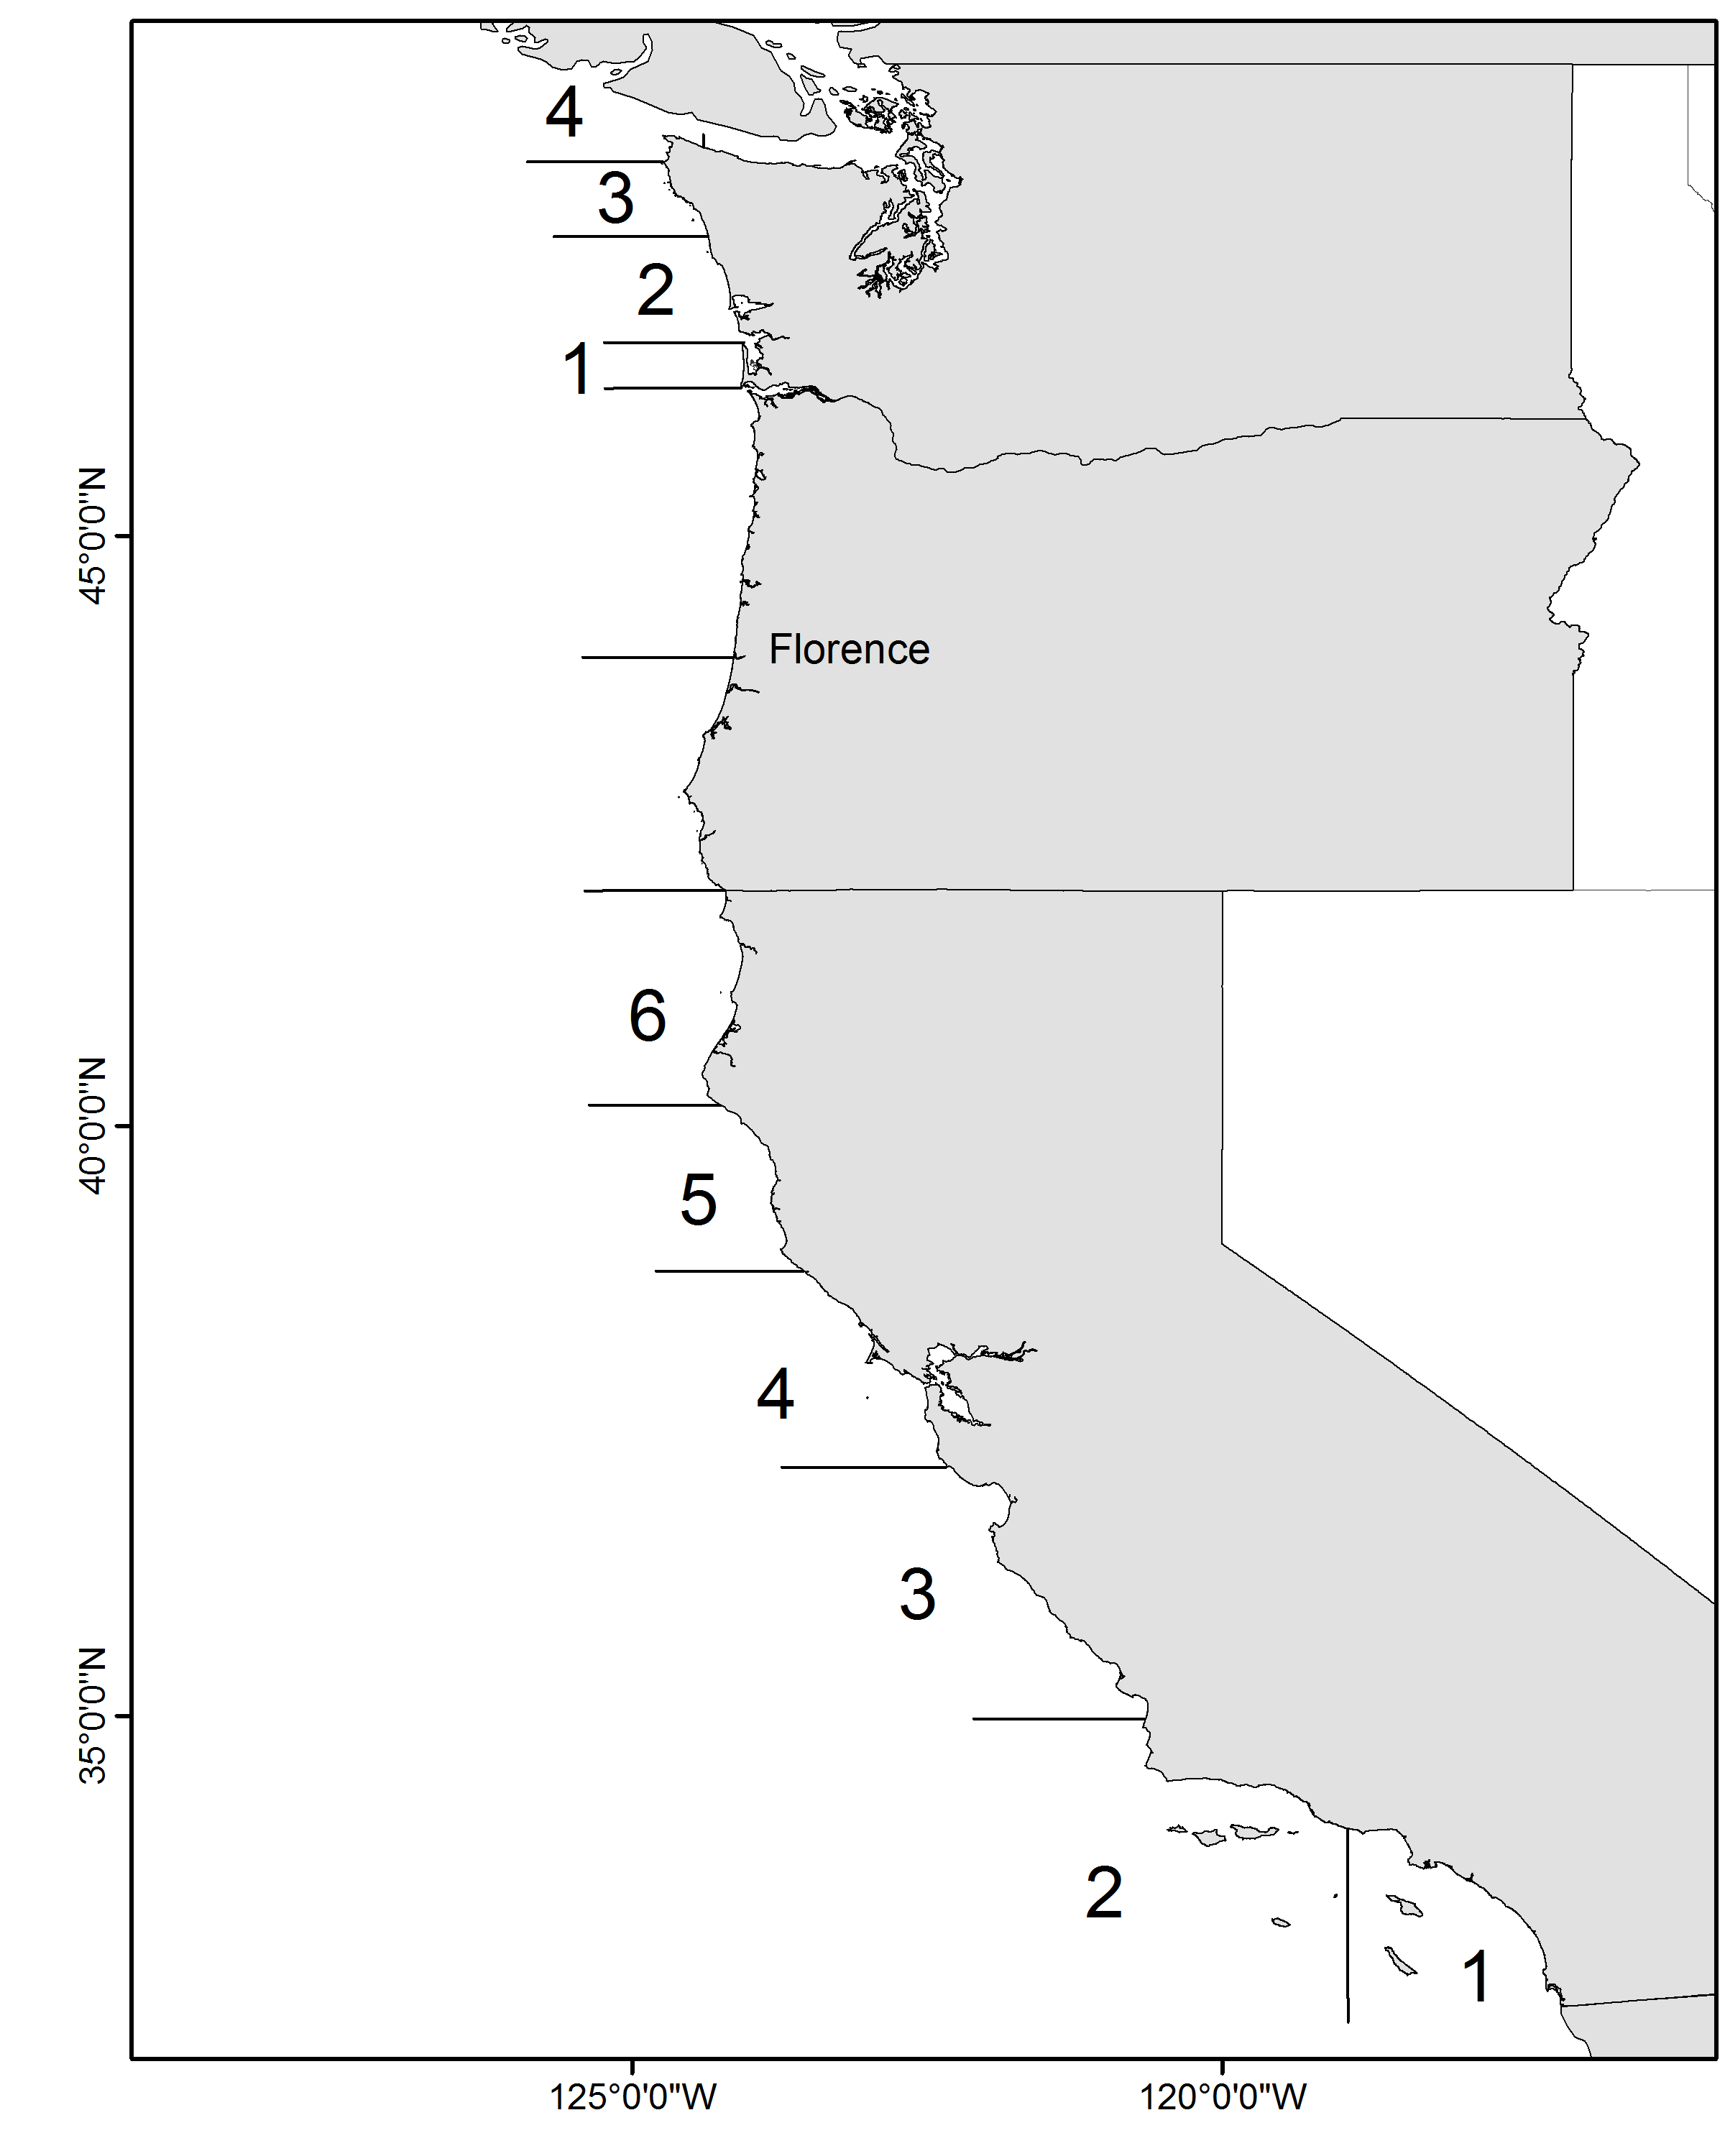
\includegraphics{Figures/boundary_map.png}
\caption{Map showing the state boundary lines for management of the
recreational fishing fleets \label{fig:boundary_map}}
\end{figure}

\begin{figure}
\centering
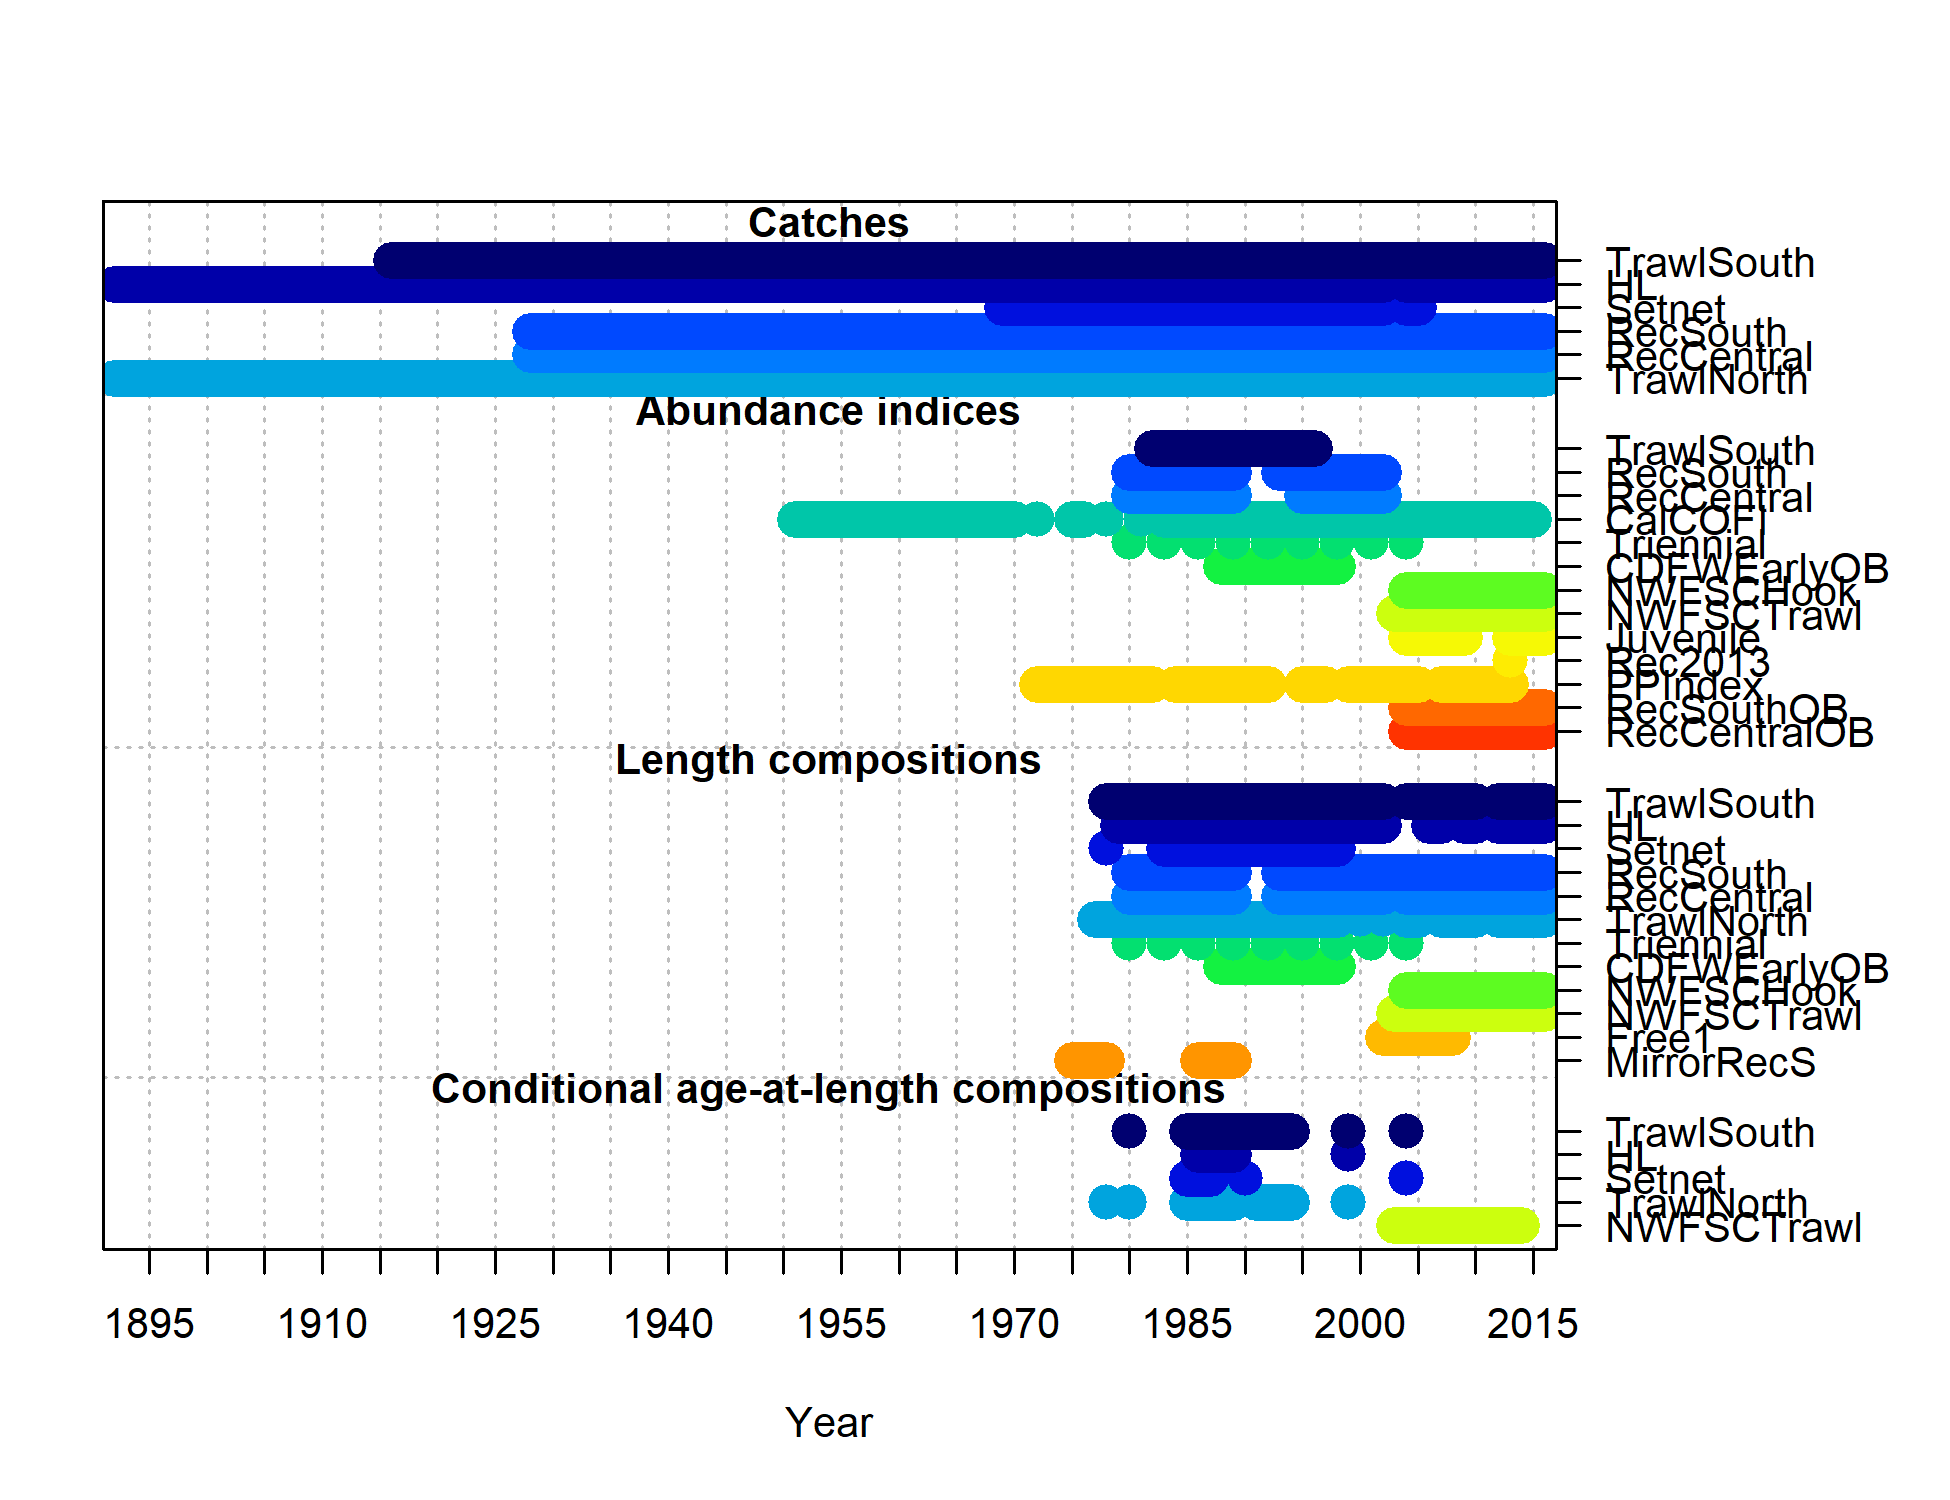
\includegraphics{r4ss/plots_mod1/data_plot.png}
\caption{Summary of data sources used in the Northern model.
\label{fig:data_plot}}
\end{figure}

\FloatBarrier

\FloatBarrier

\FloatBarrier
<!-- ********************************************************************** -->

\FloatBarrier

\FloatBarrier

\FloatBarrier

\FloatBarrier

\begin{figure}
\centering
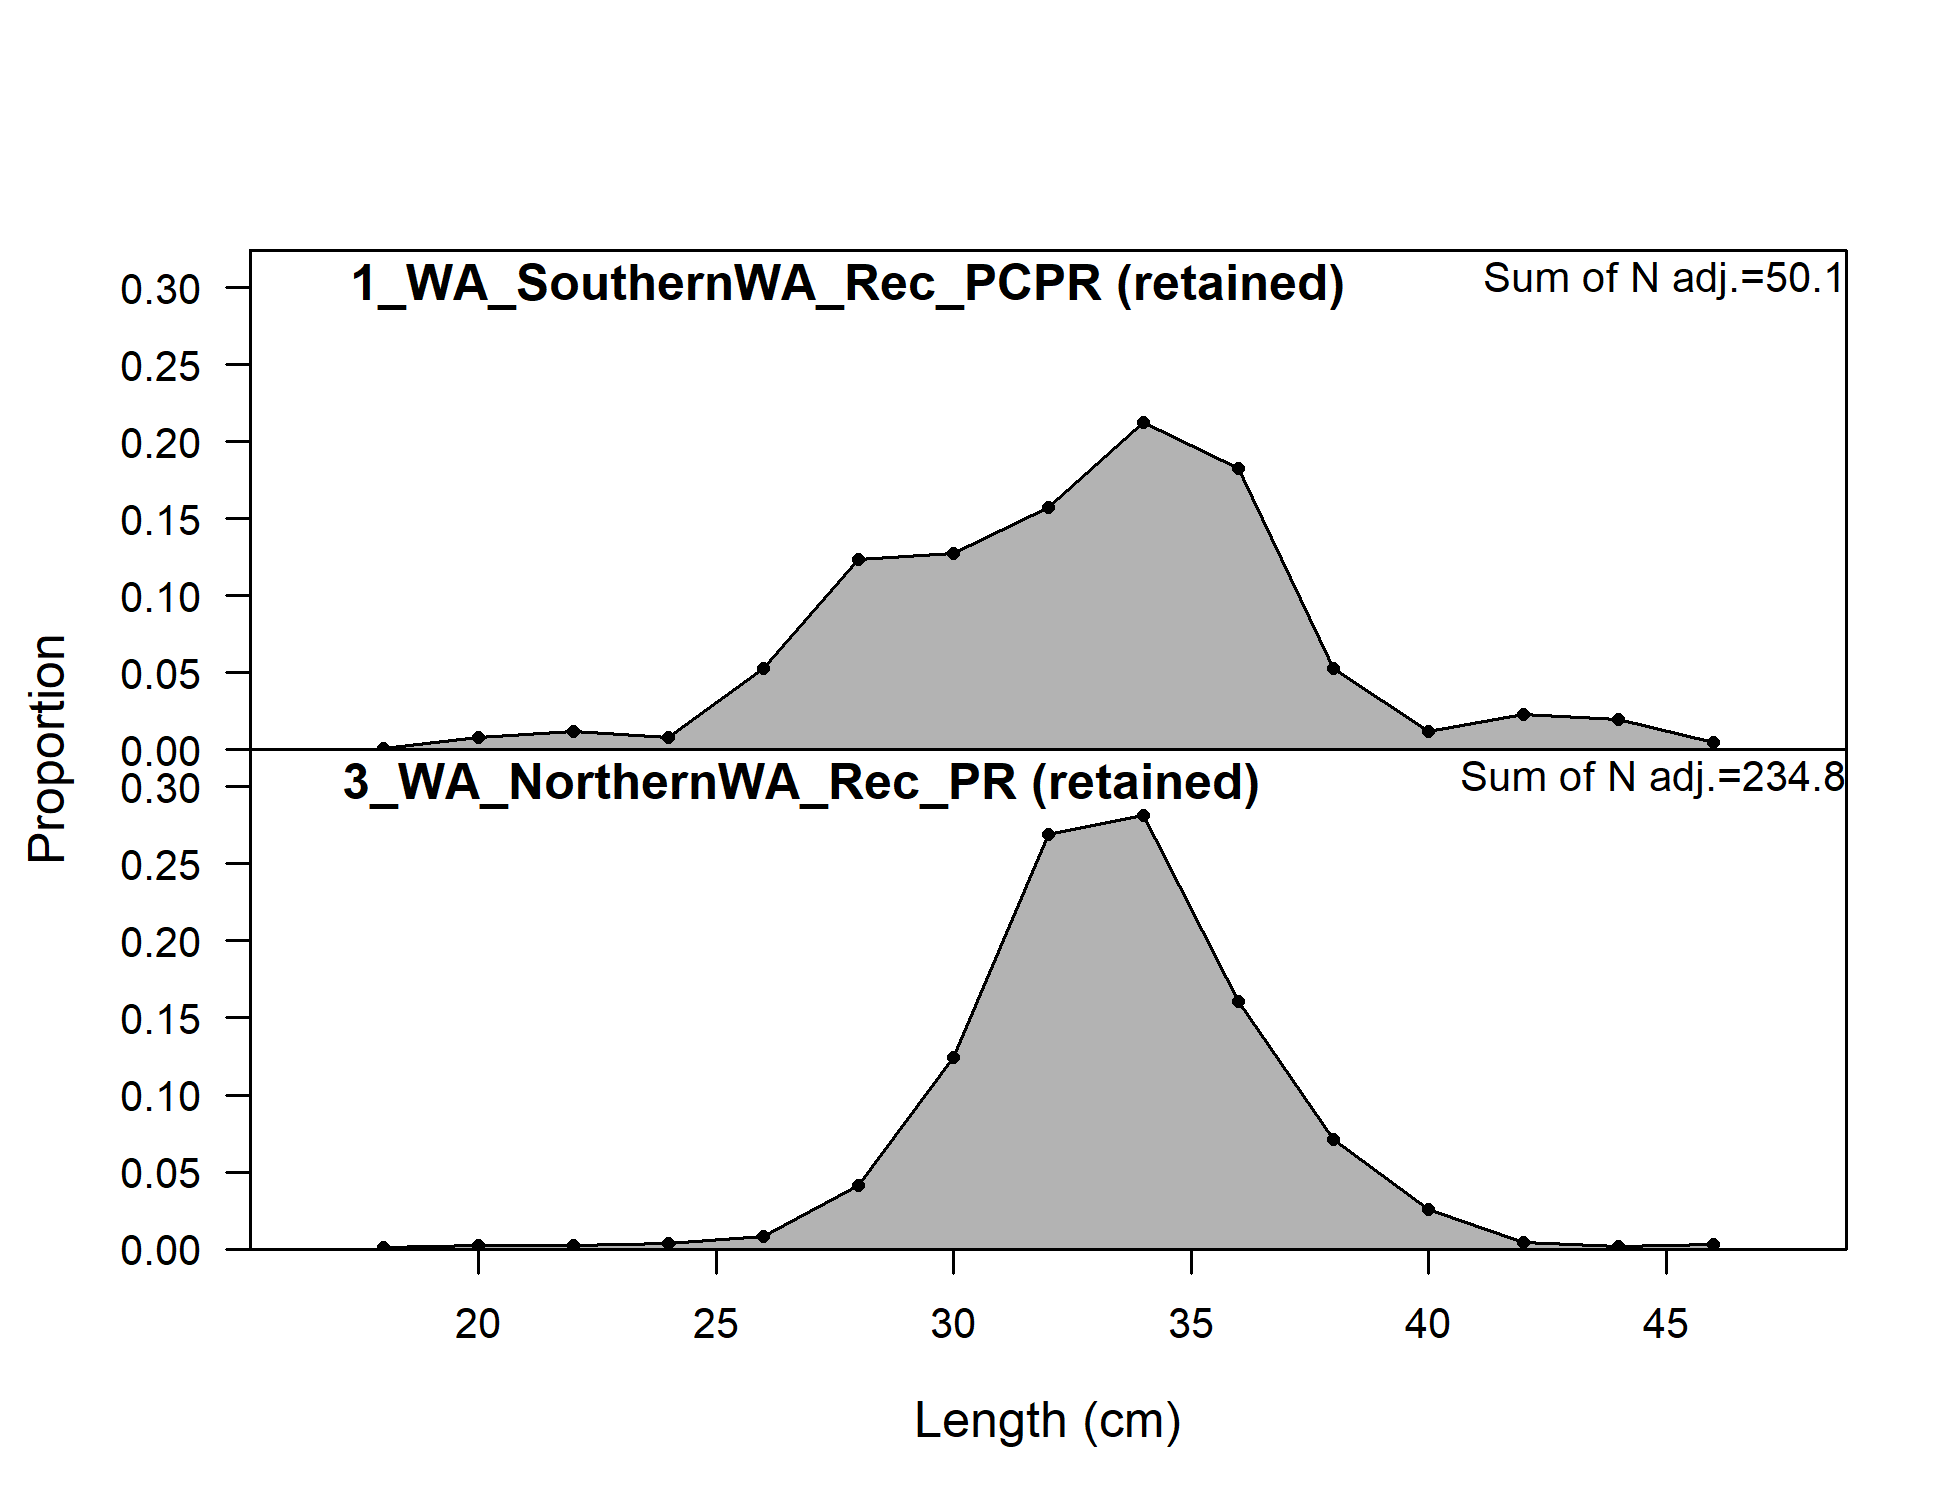
\includegraphics{r4ss/plots_mod1/comp_lendat__aggregated_across_time.png}
\caption{Length comp data, aggregated across time by fleet. Labels
`retained' and `discard' indicate discarded or retained sampled for each
fleet. Panels without this designation represent the whole catch.
\label{fig:comp_lendat_aggregated_across_time}}
\end{figure}

\FloatBarrier

\FloatBarrier

\FloatBarrier

\FloatBarrier

\begin{figure}
\centering
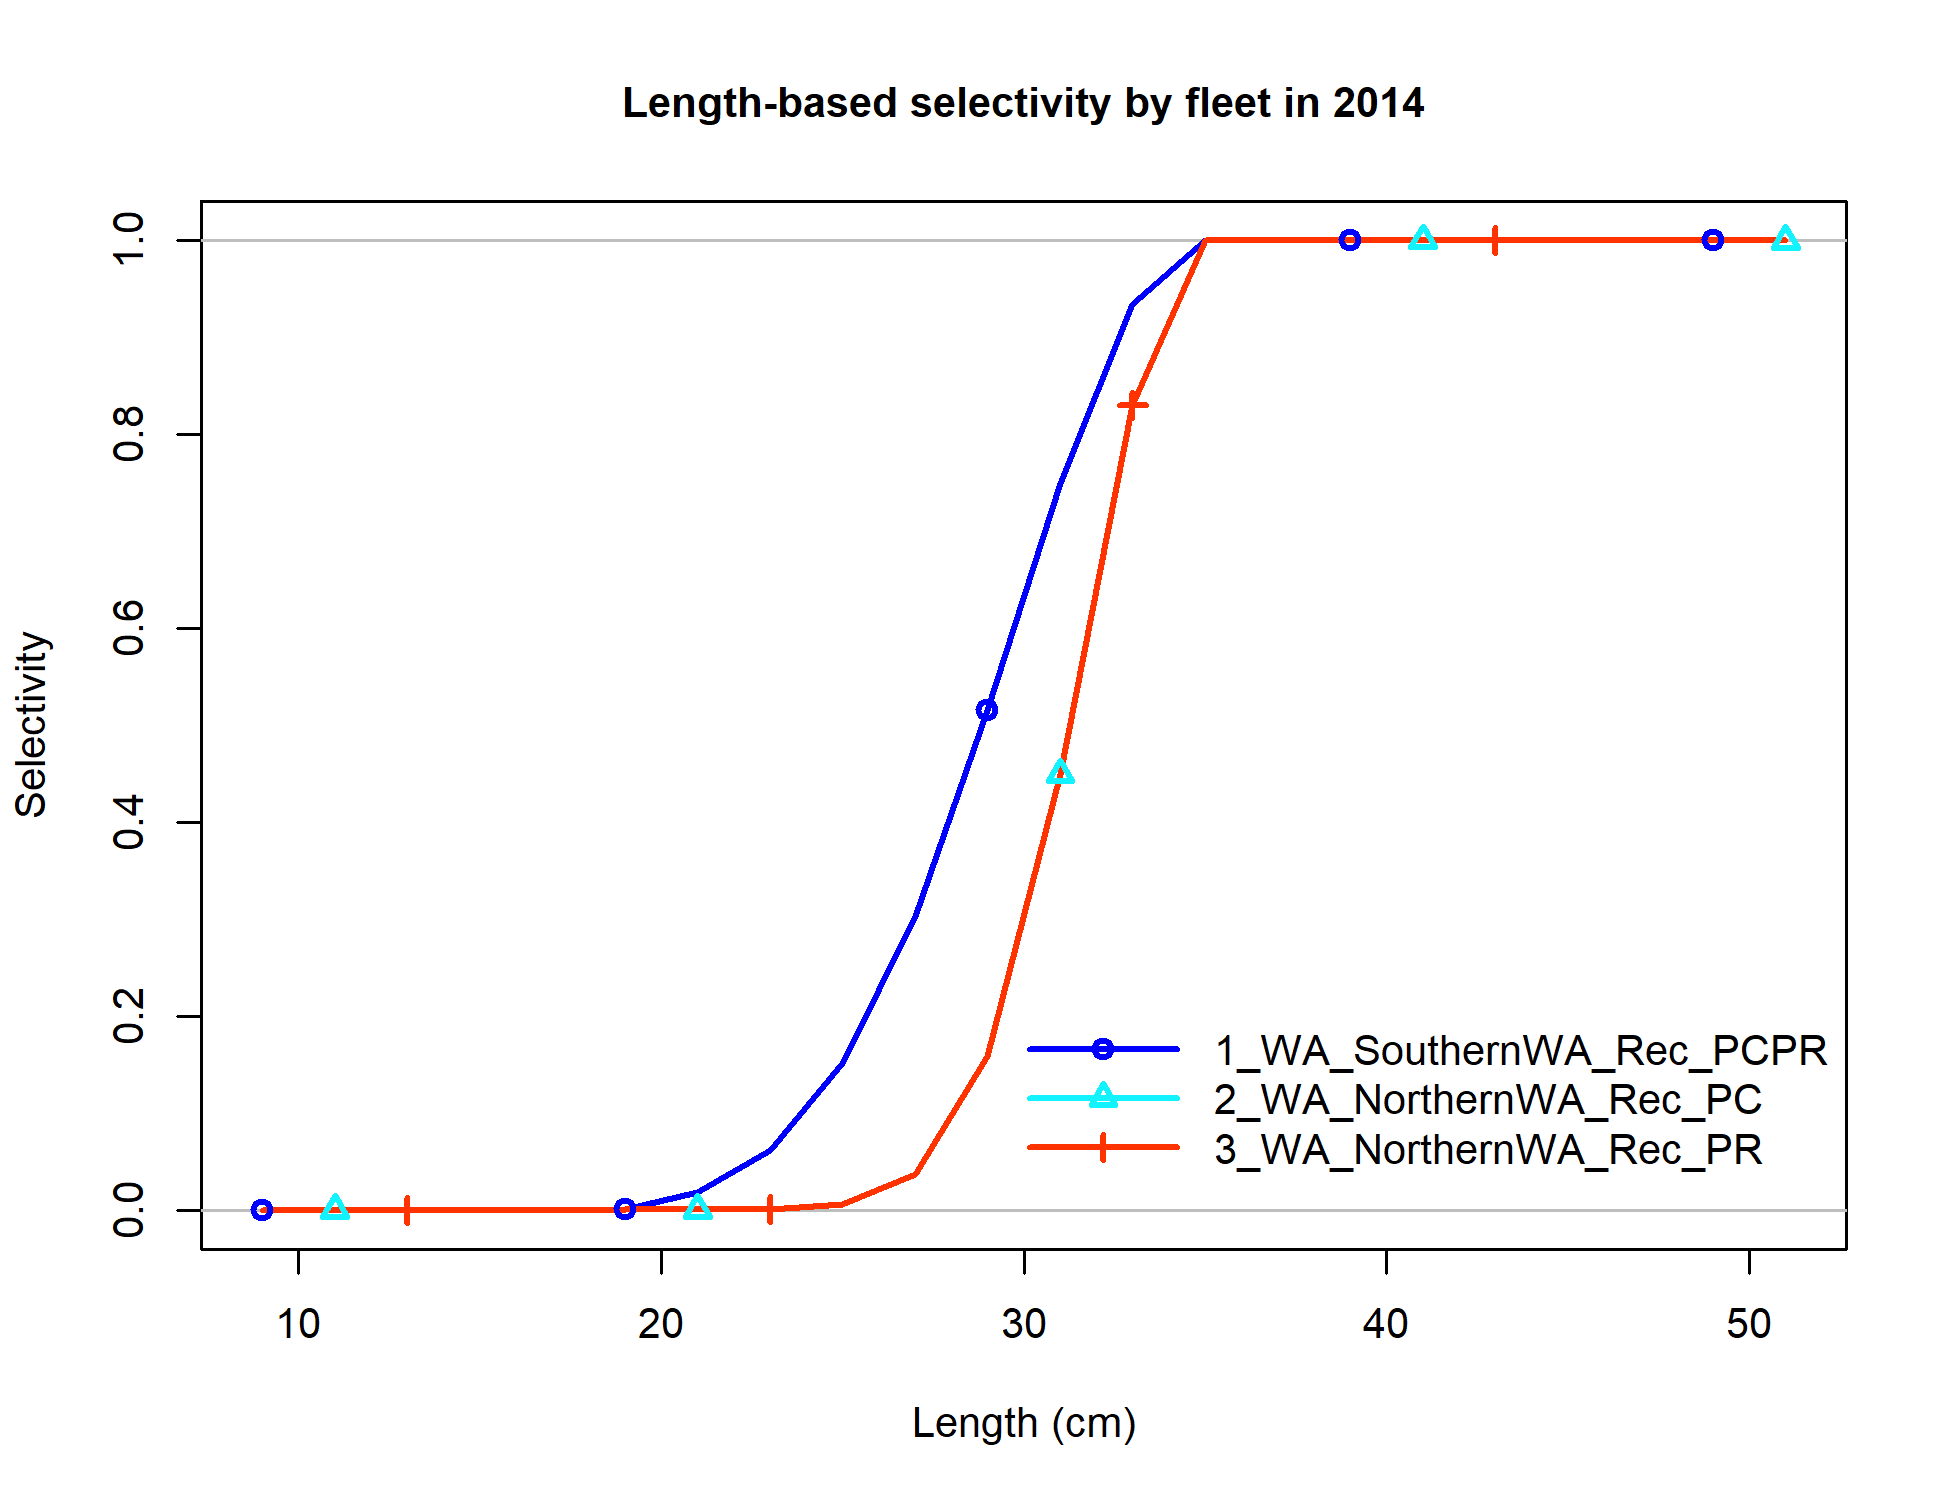
\includegraphics{r4ss/plots_mod1/sel01_multiple_fleets_length1.png}
\caption{Selectivity at length for all of the fleets in the base model.
\label{fig:sel01_multiple_fleets_length1}}
\end{figure}

\FloatBarrier

\begin{figure}
\centering
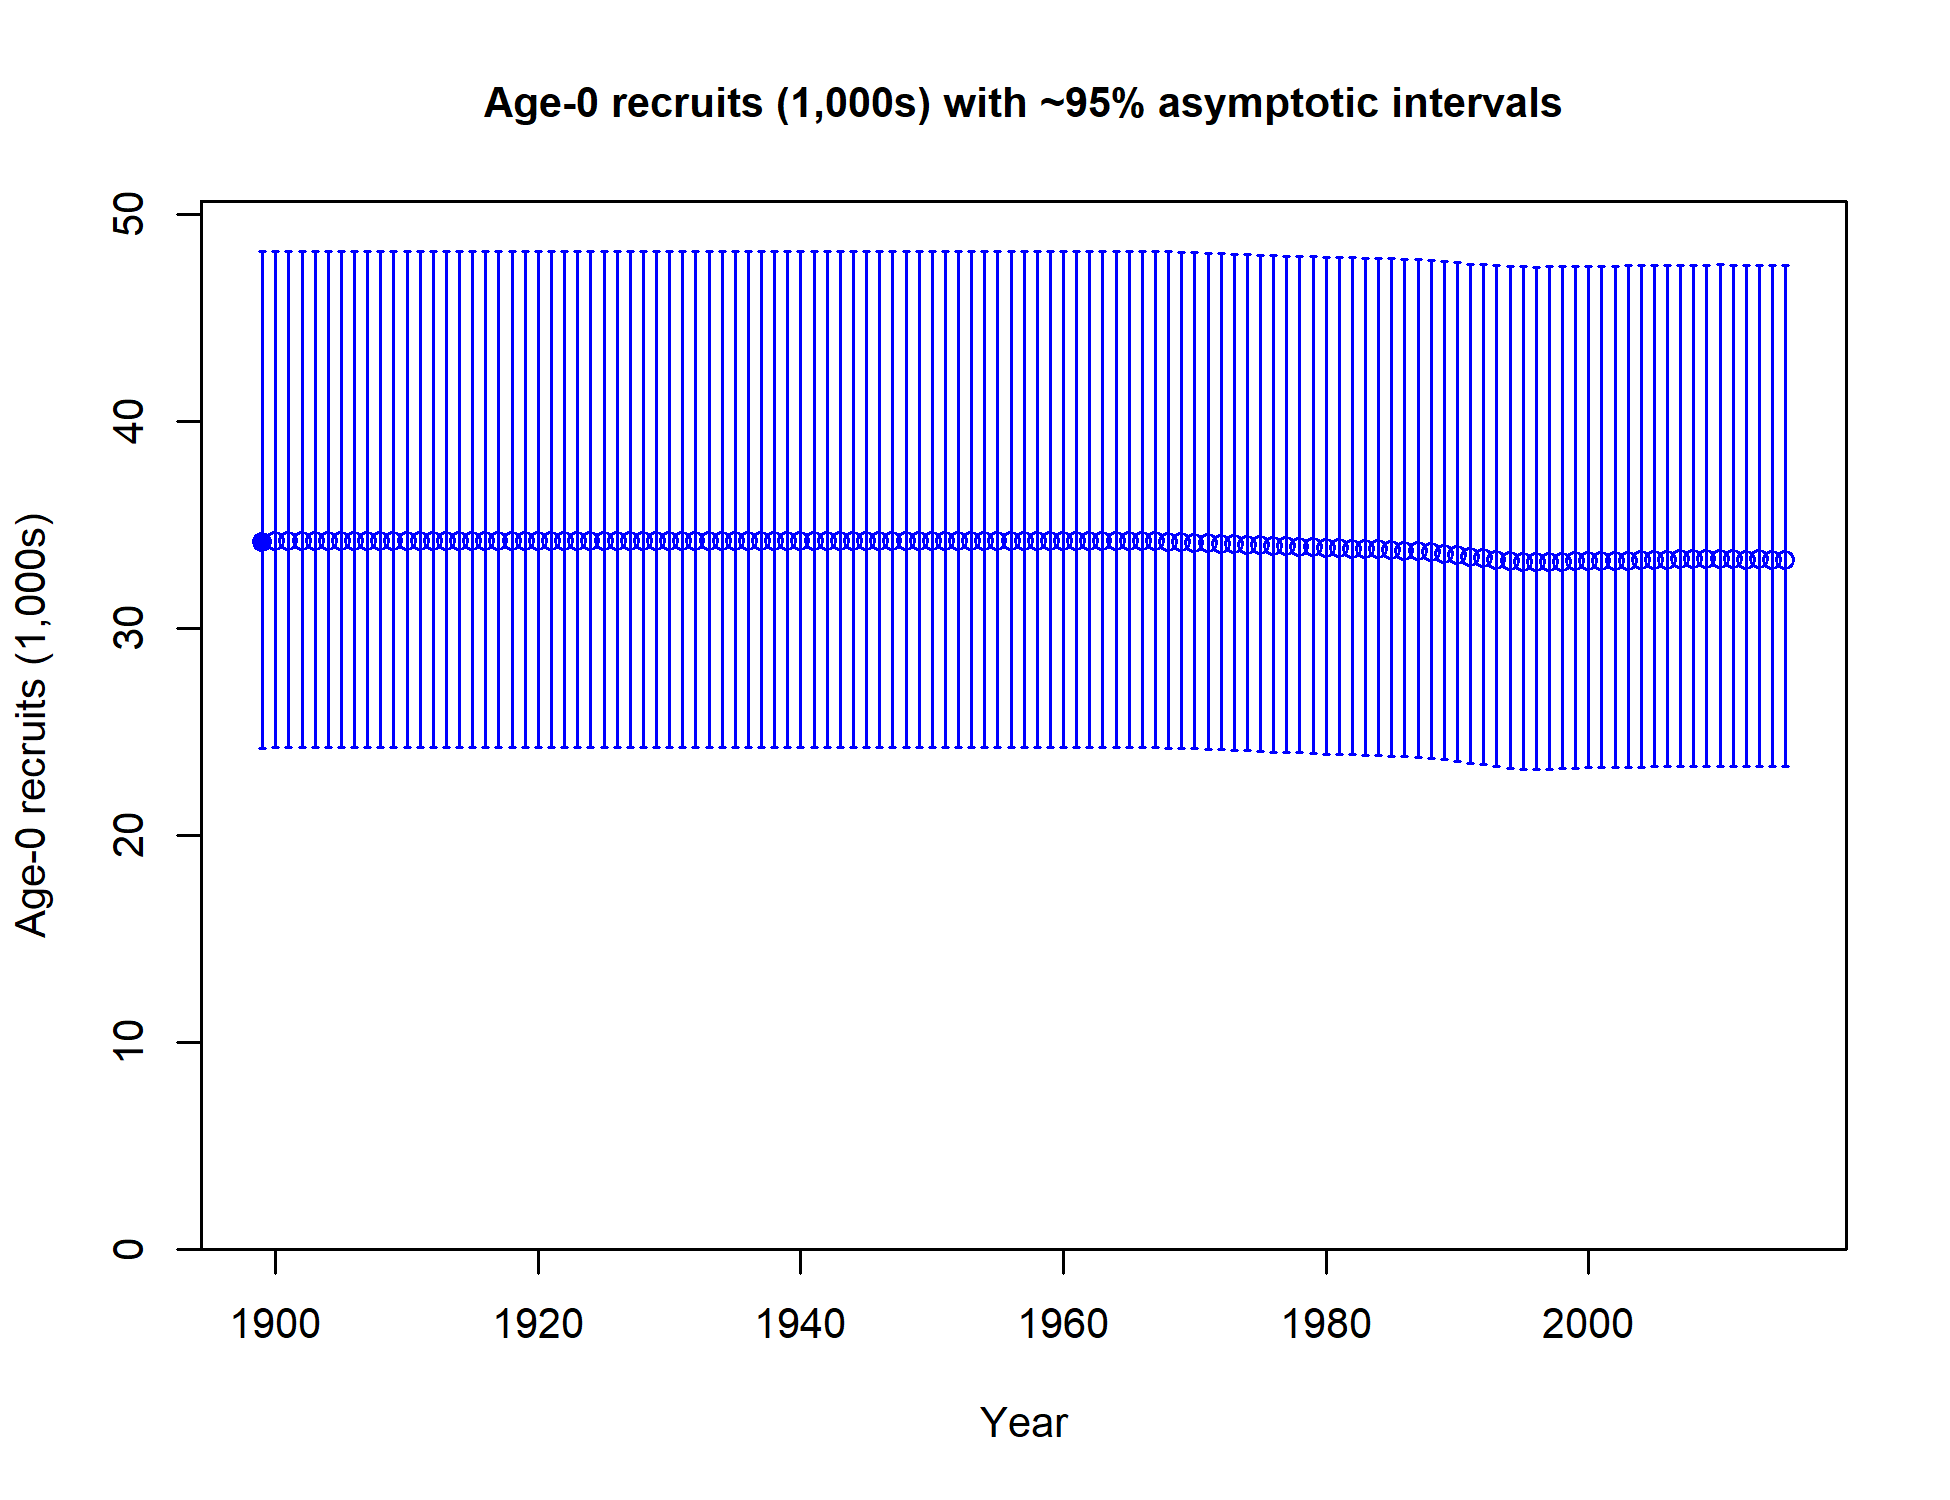
\includegraphics{r4ss/plots_mod1/ts11_Age-0_recruits_(1000s)_with_95_asymptotic_intervals.png}
\caption{Estimated time-series of recruitment for China rockfish.
\label{fig:ts11_Age-0_recruits_(1000s)_with_95_asymptotic_intervals}}
\end{figure}

\begin{figure}
\centering
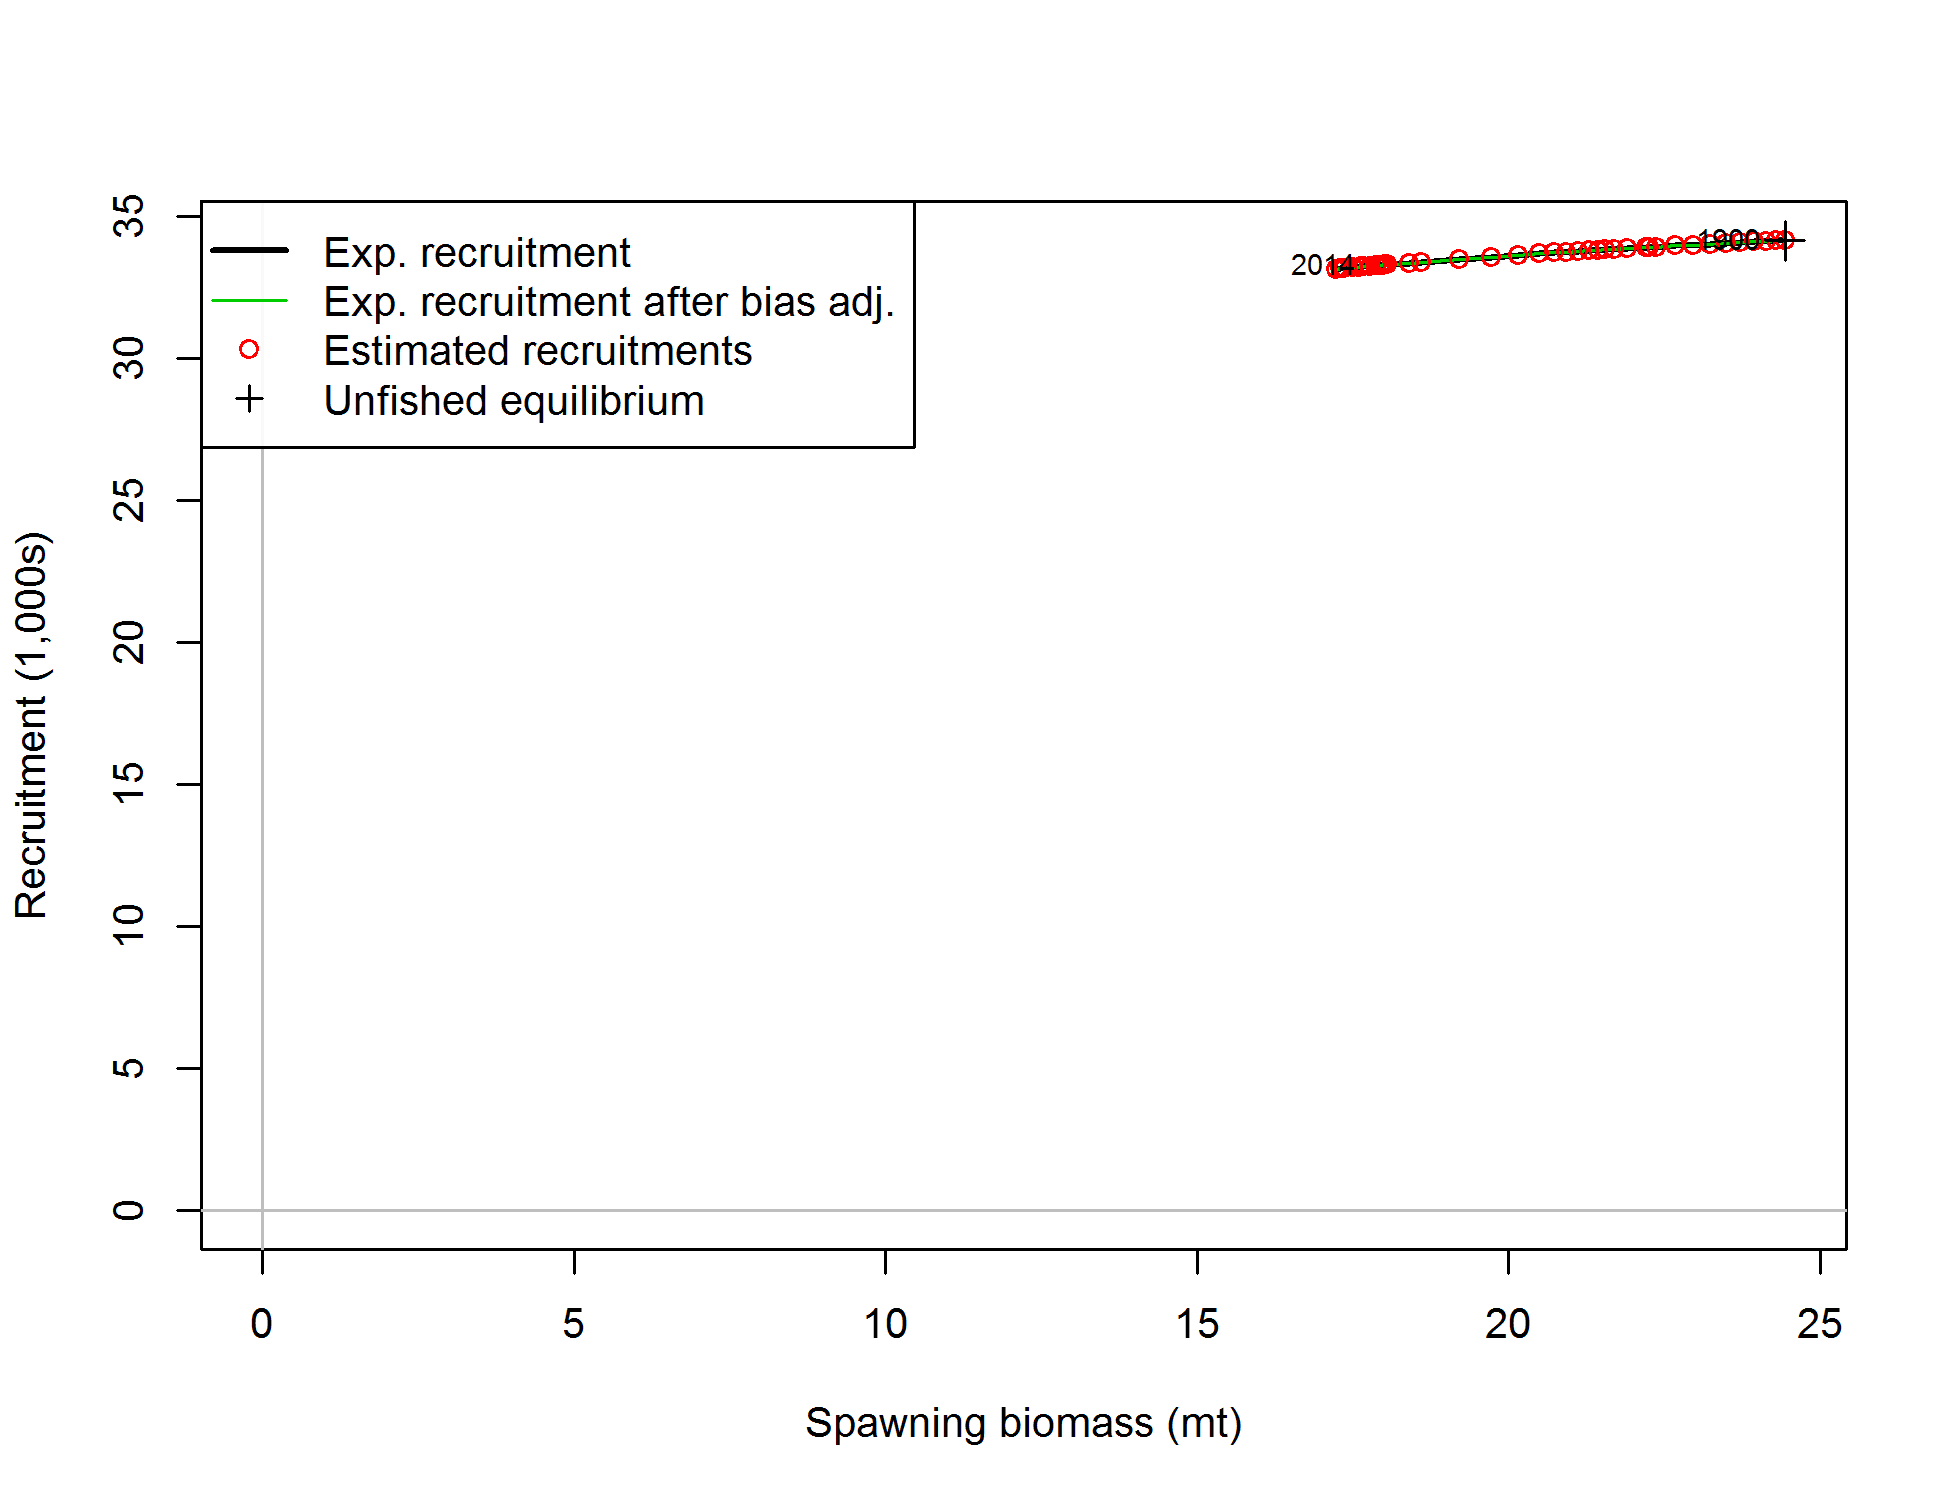
\includegraphics{r4ss/plots_mod1/SR_curve2.png}
\caption{Estimated recruitment (red circles) and the assumed
stock-recruit relationship (black line) for China rockfish. The green
line shows the effect of the bias correction for the lognormal
distribution. \label{fig:SR_curve2}}
\end{figure}

\FloatBarrier

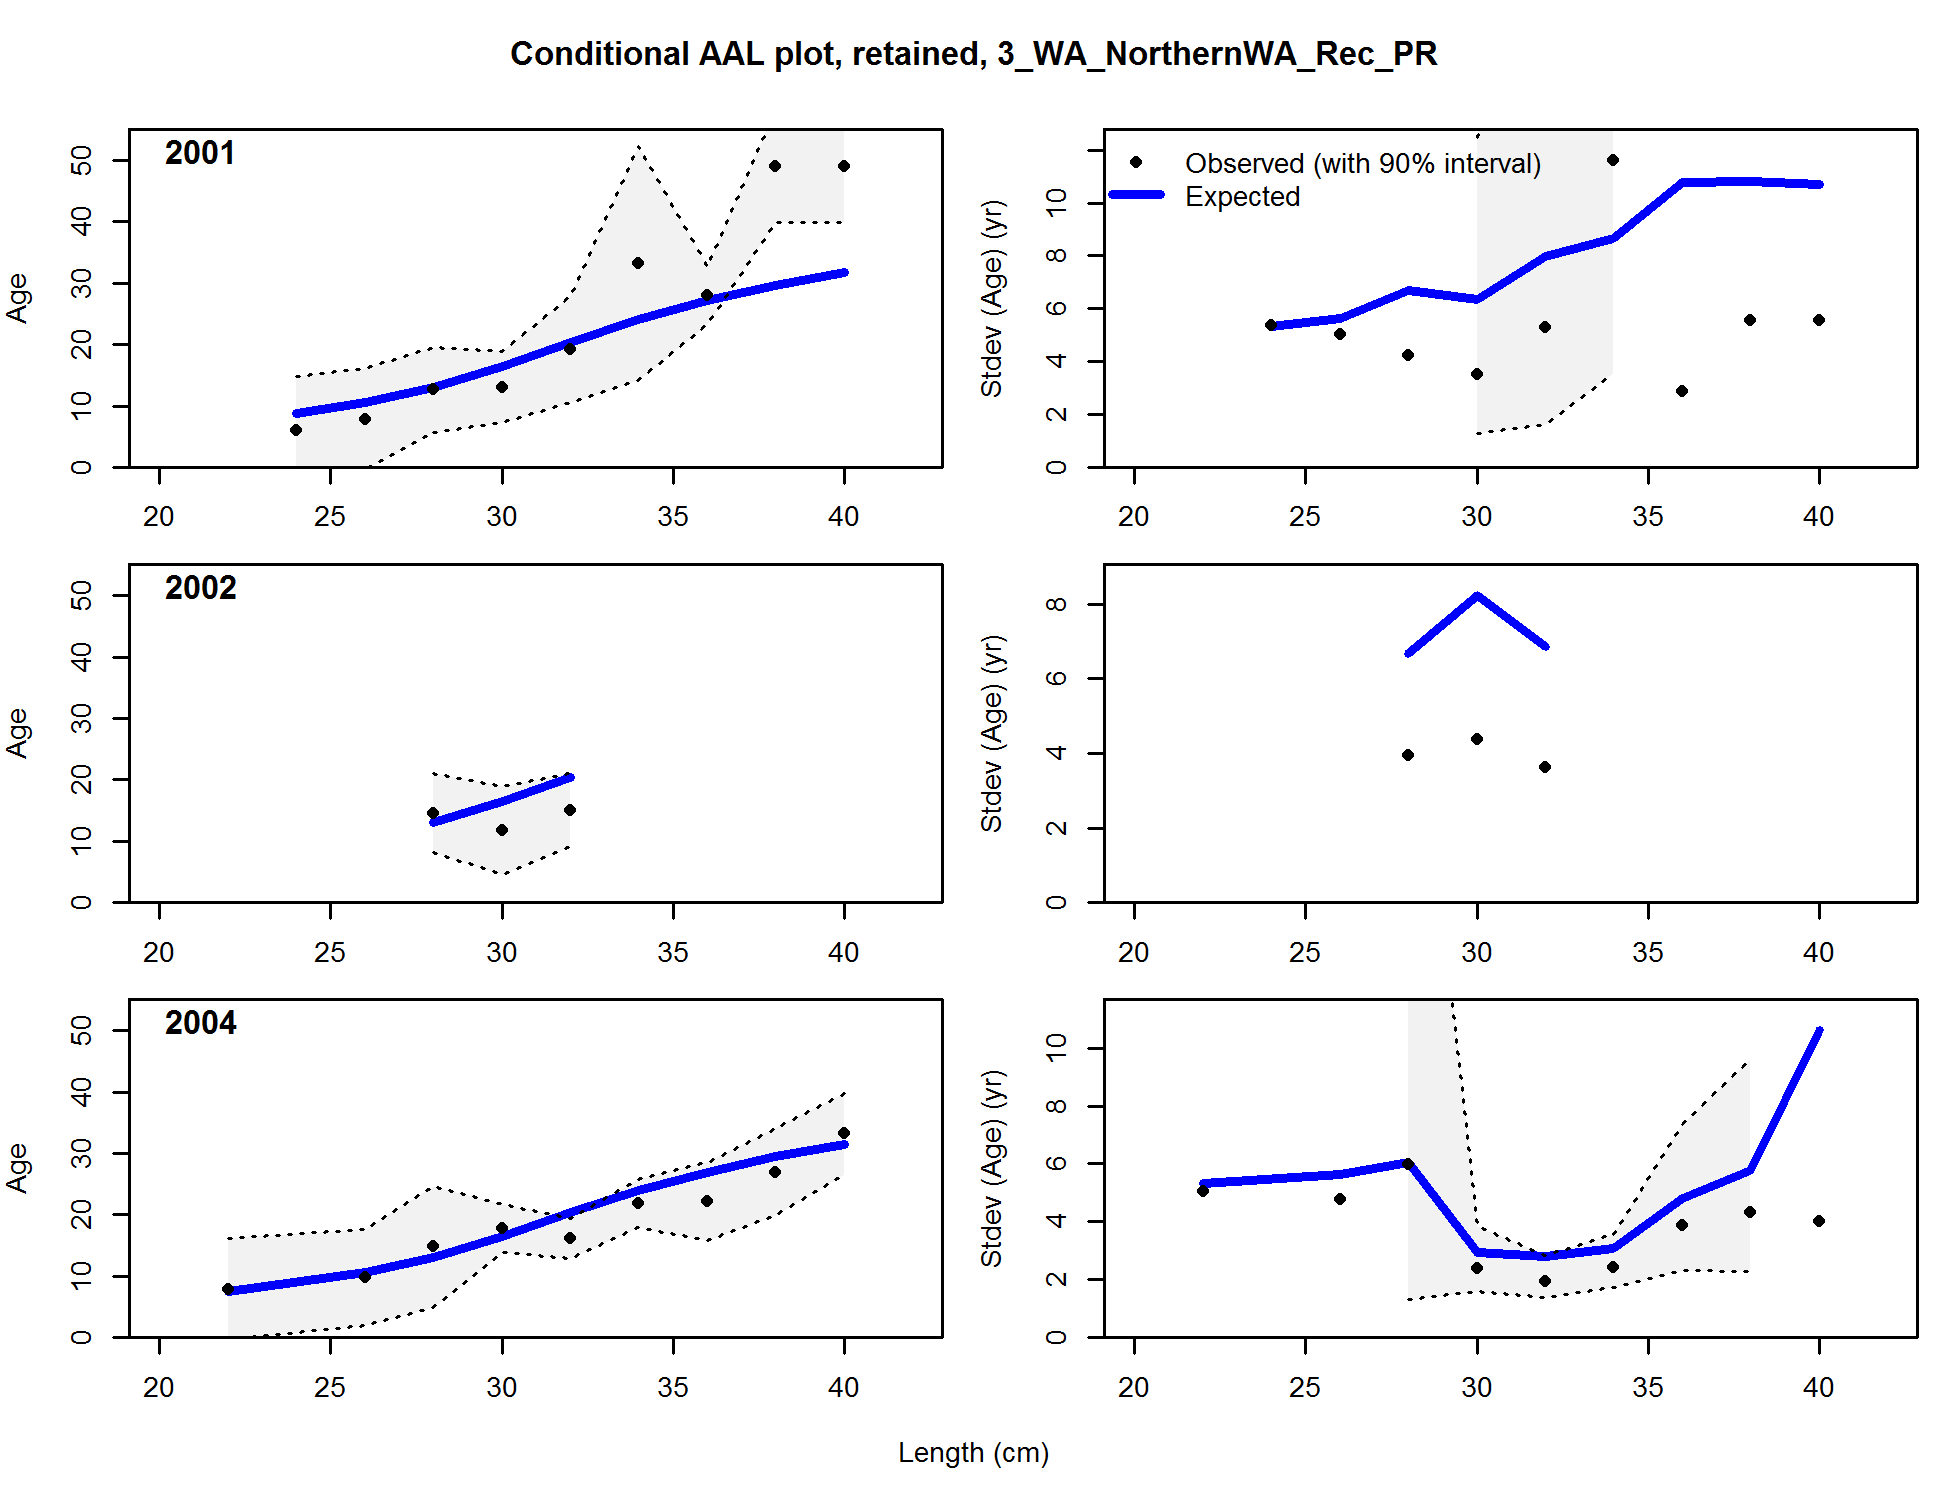
\includegraphics{./r4ss/plots_mod1/comp_condAALfit_Andre_plotsflt3mkt2_page2.png}

\begin{center} 

              Figure continued from previous page 

             \end{center}

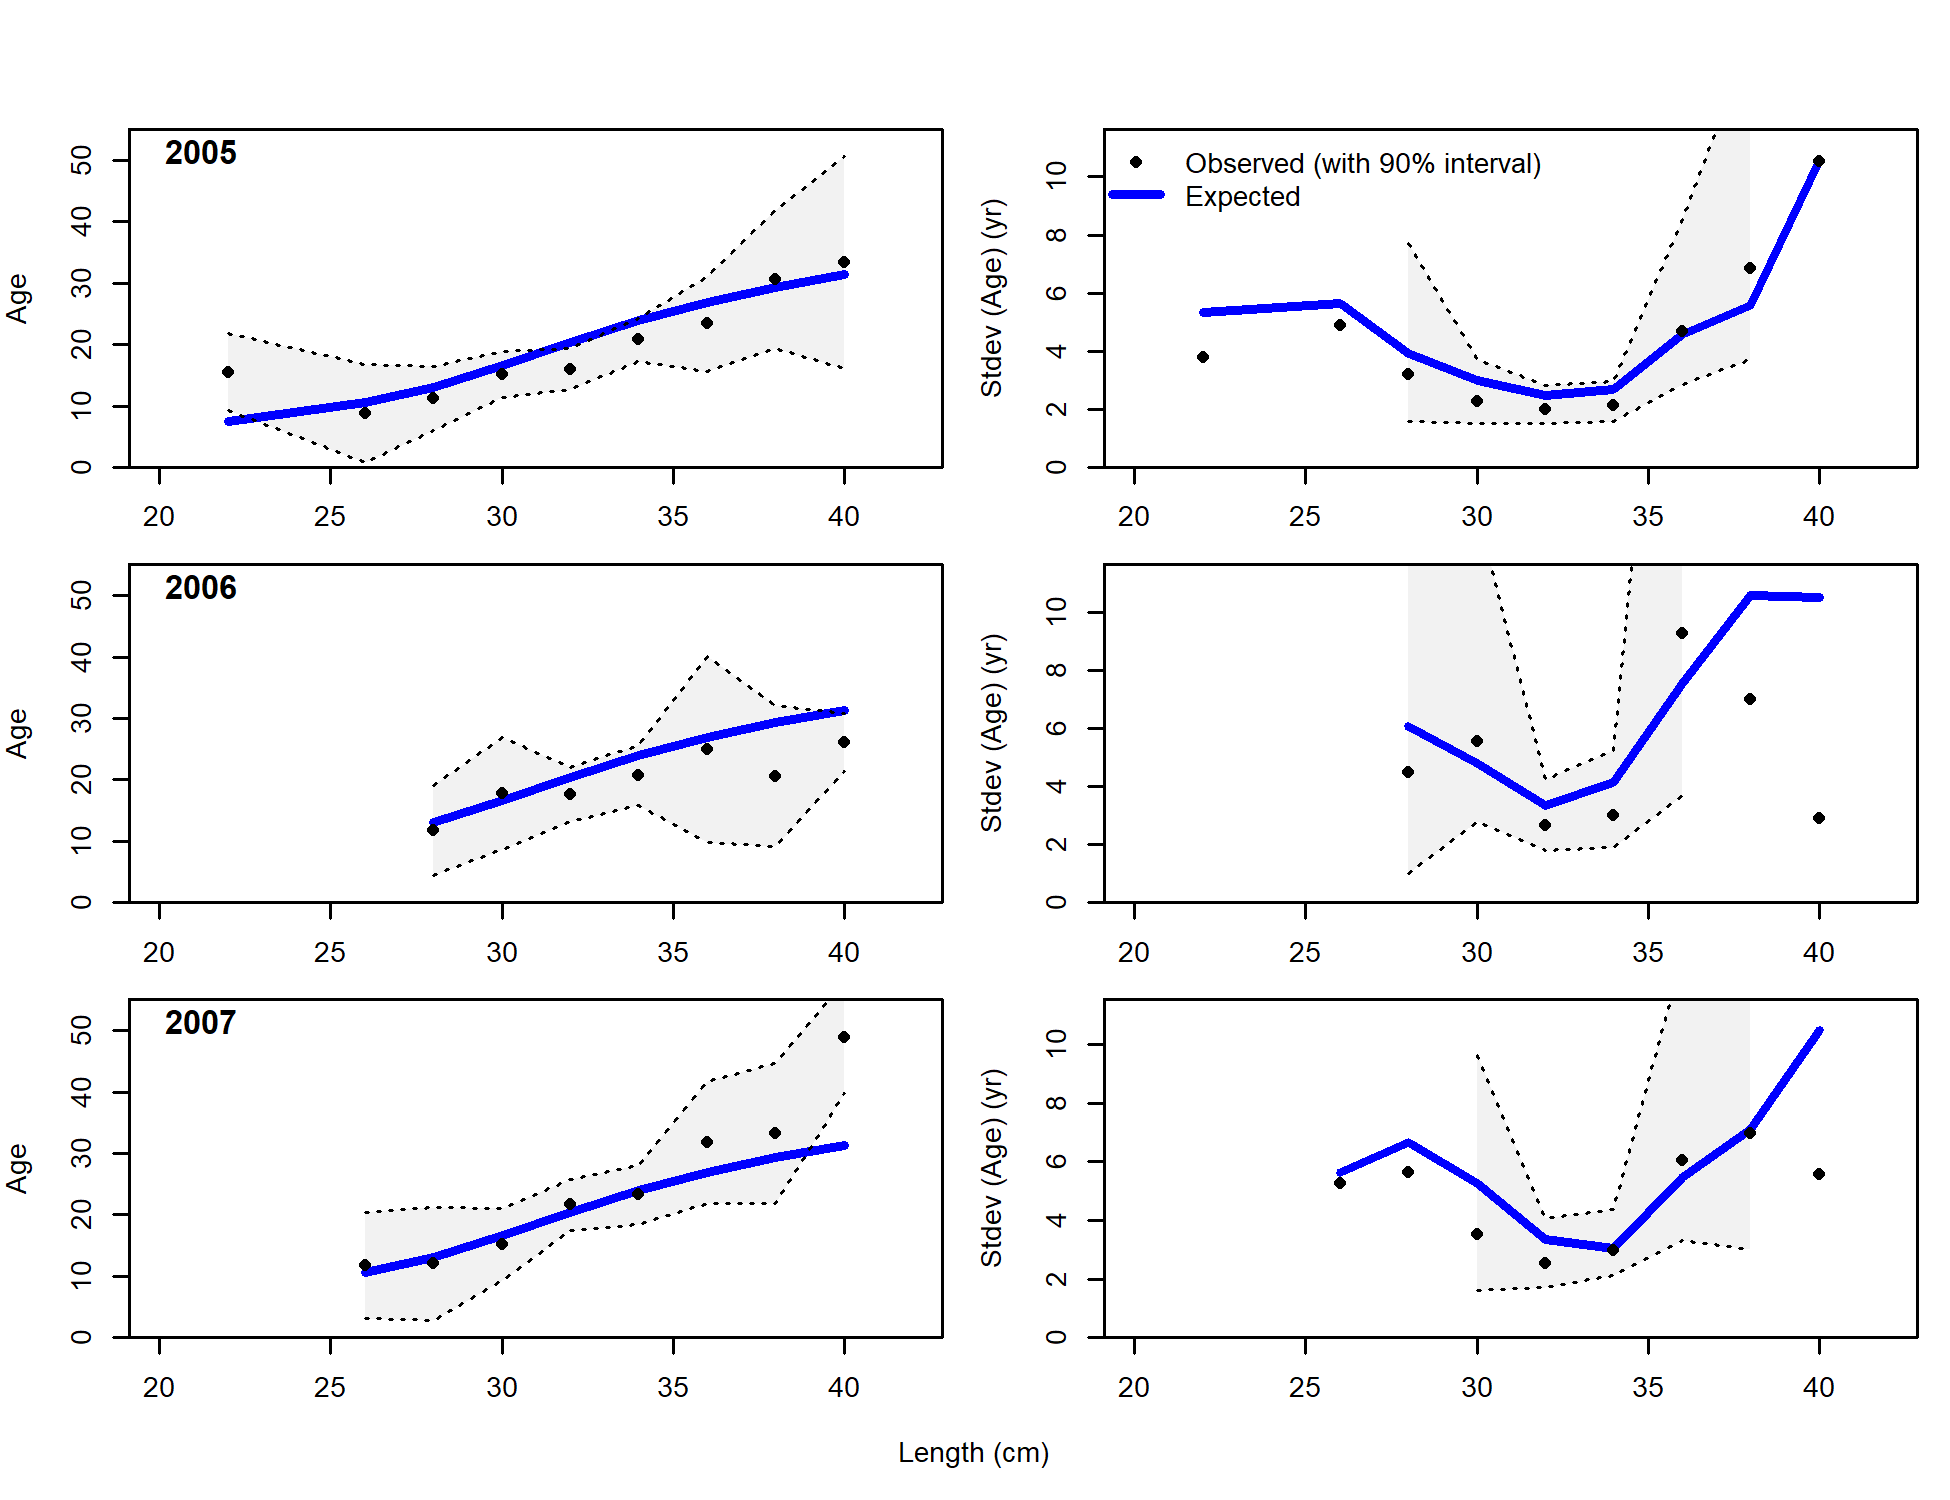
\includegraphics{./r4ss/plots_mod1/comp_condAALfit_Andre_plotsflt3mkt2_page3.png}

\begin{center} 

              Figure continued from previous page 

             \end{center}

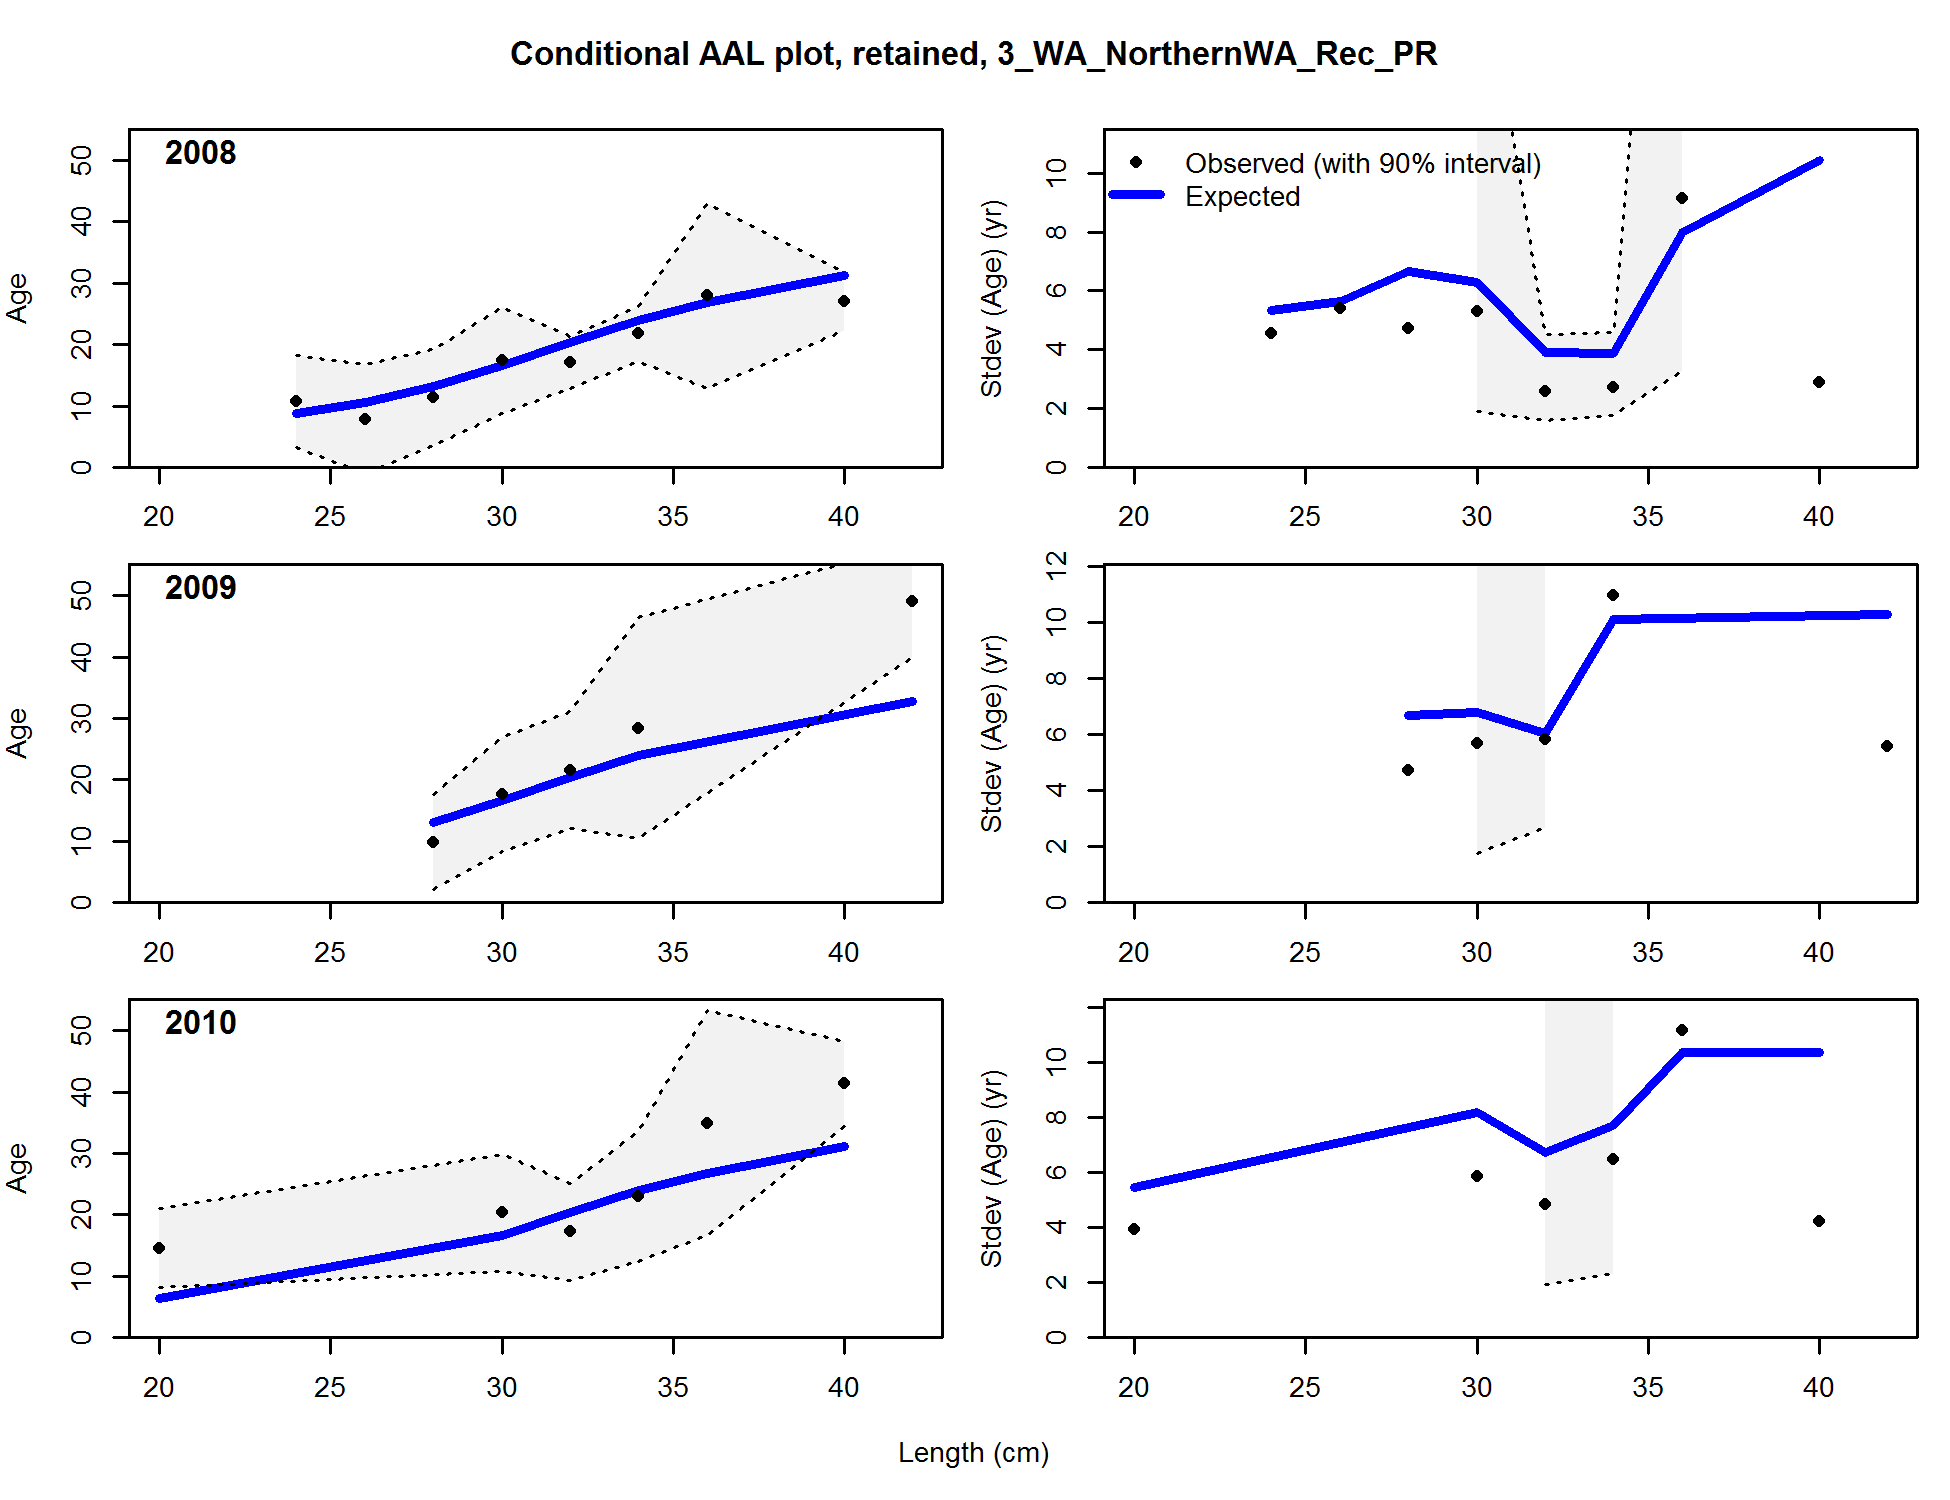
\includegraphics{./r4ss/plots_mod1/comp_condAALfit_Andre_plotsflt3mkt2_page4.png}

\begin{center} 

              Figure continued from previous page 

             \end{center}

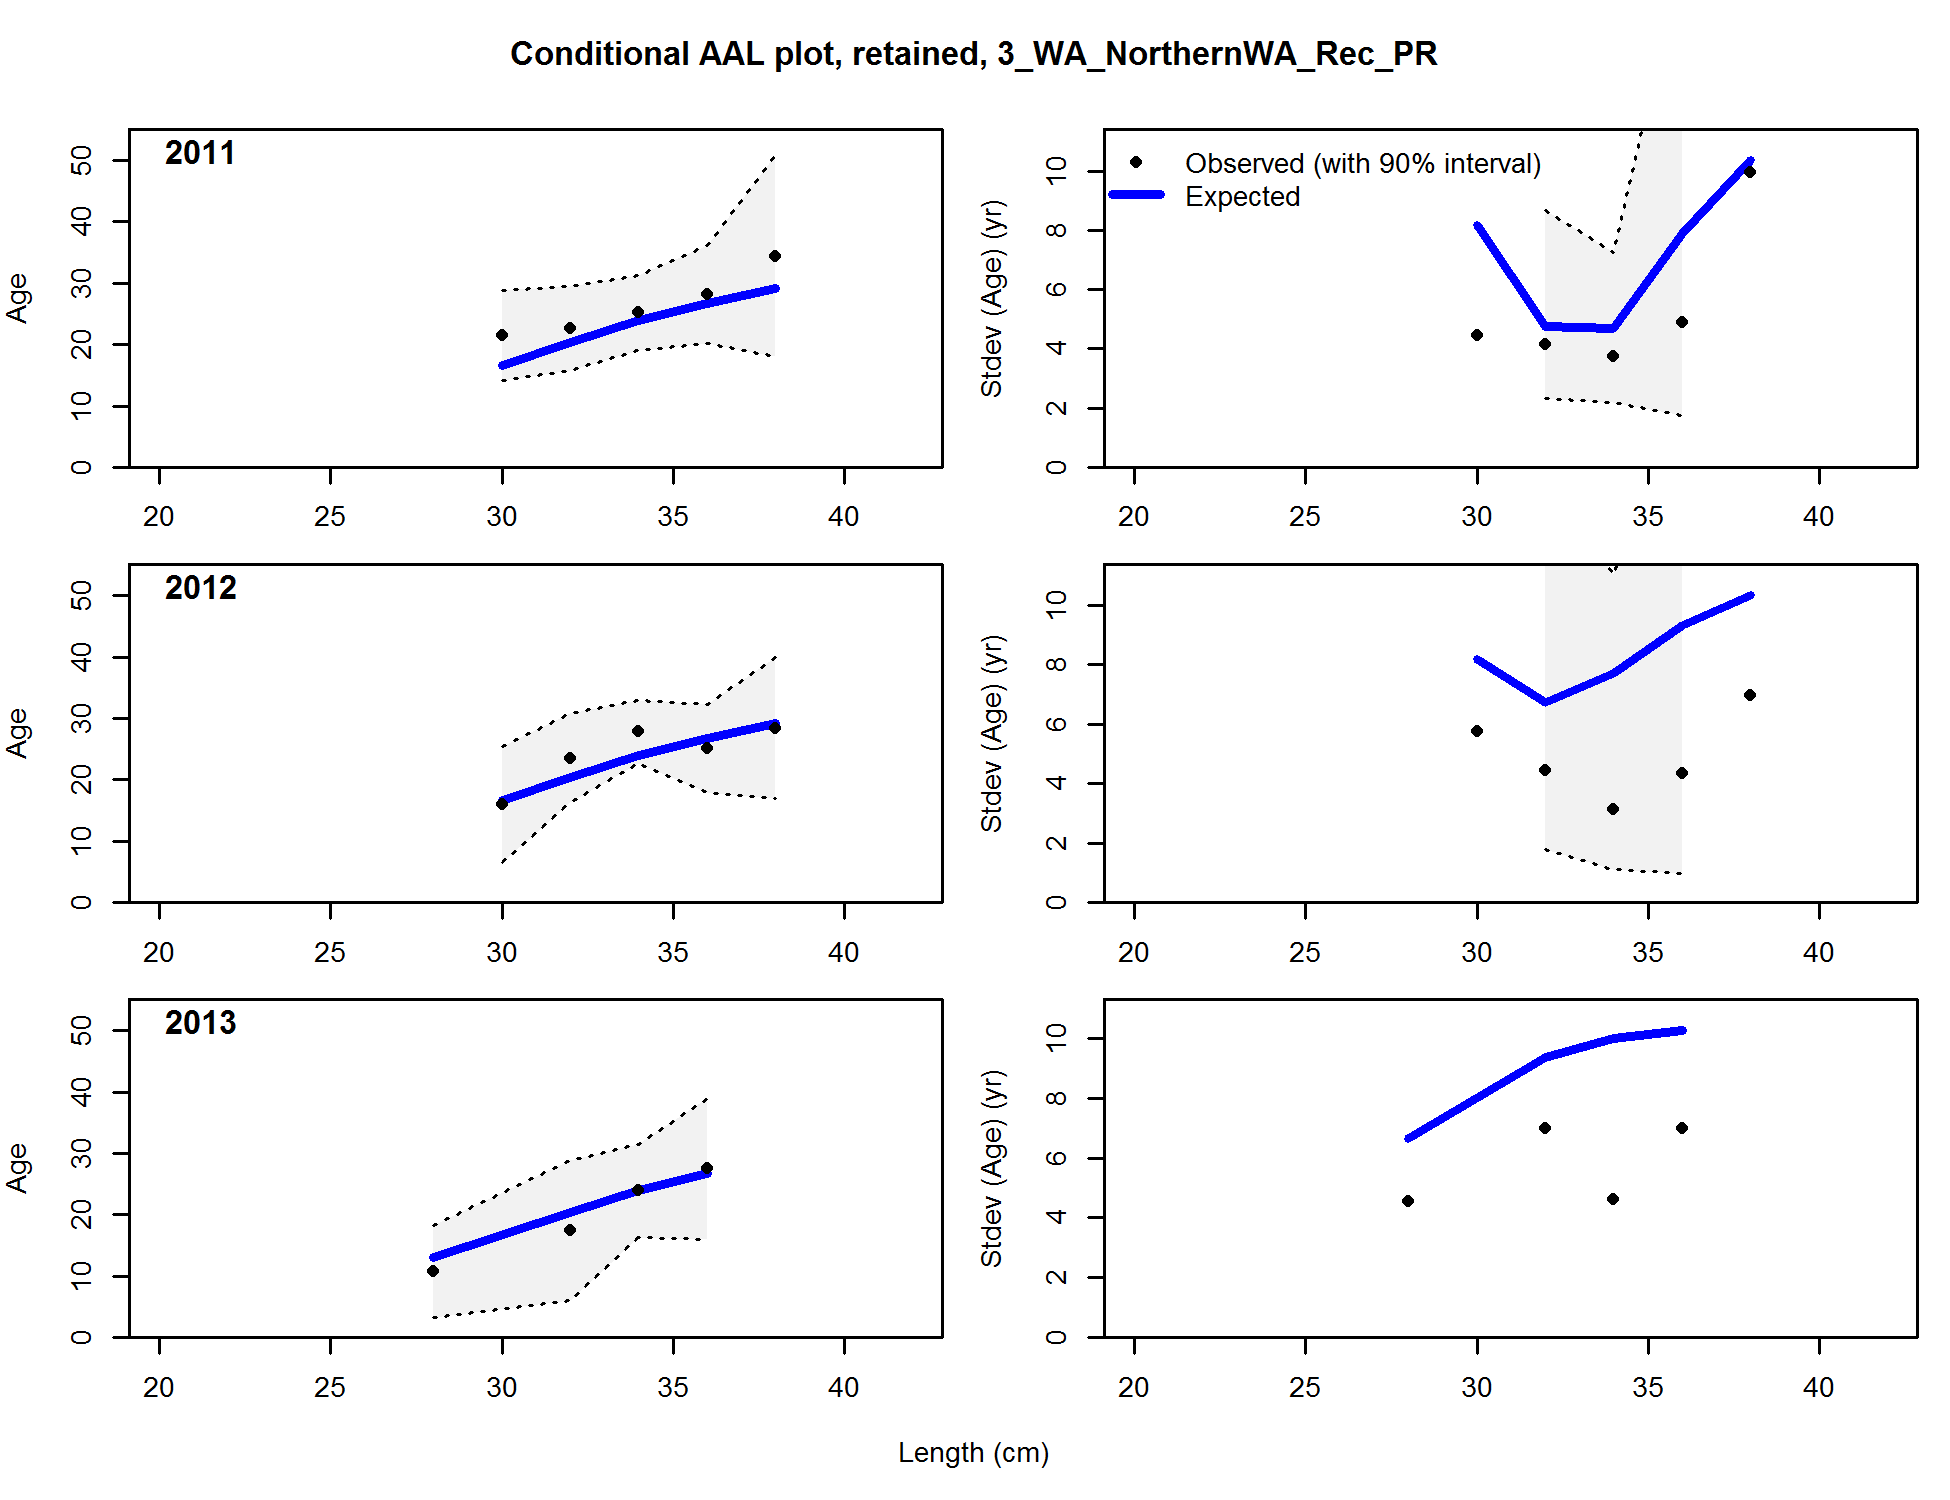
\includegraphics{./r4ss/plots_mod1/comp_condAALfit_Andre_plotsflt3mkt2_page5.png}

\begin{center} 

              Figure continued from previous page 

             \end{center}

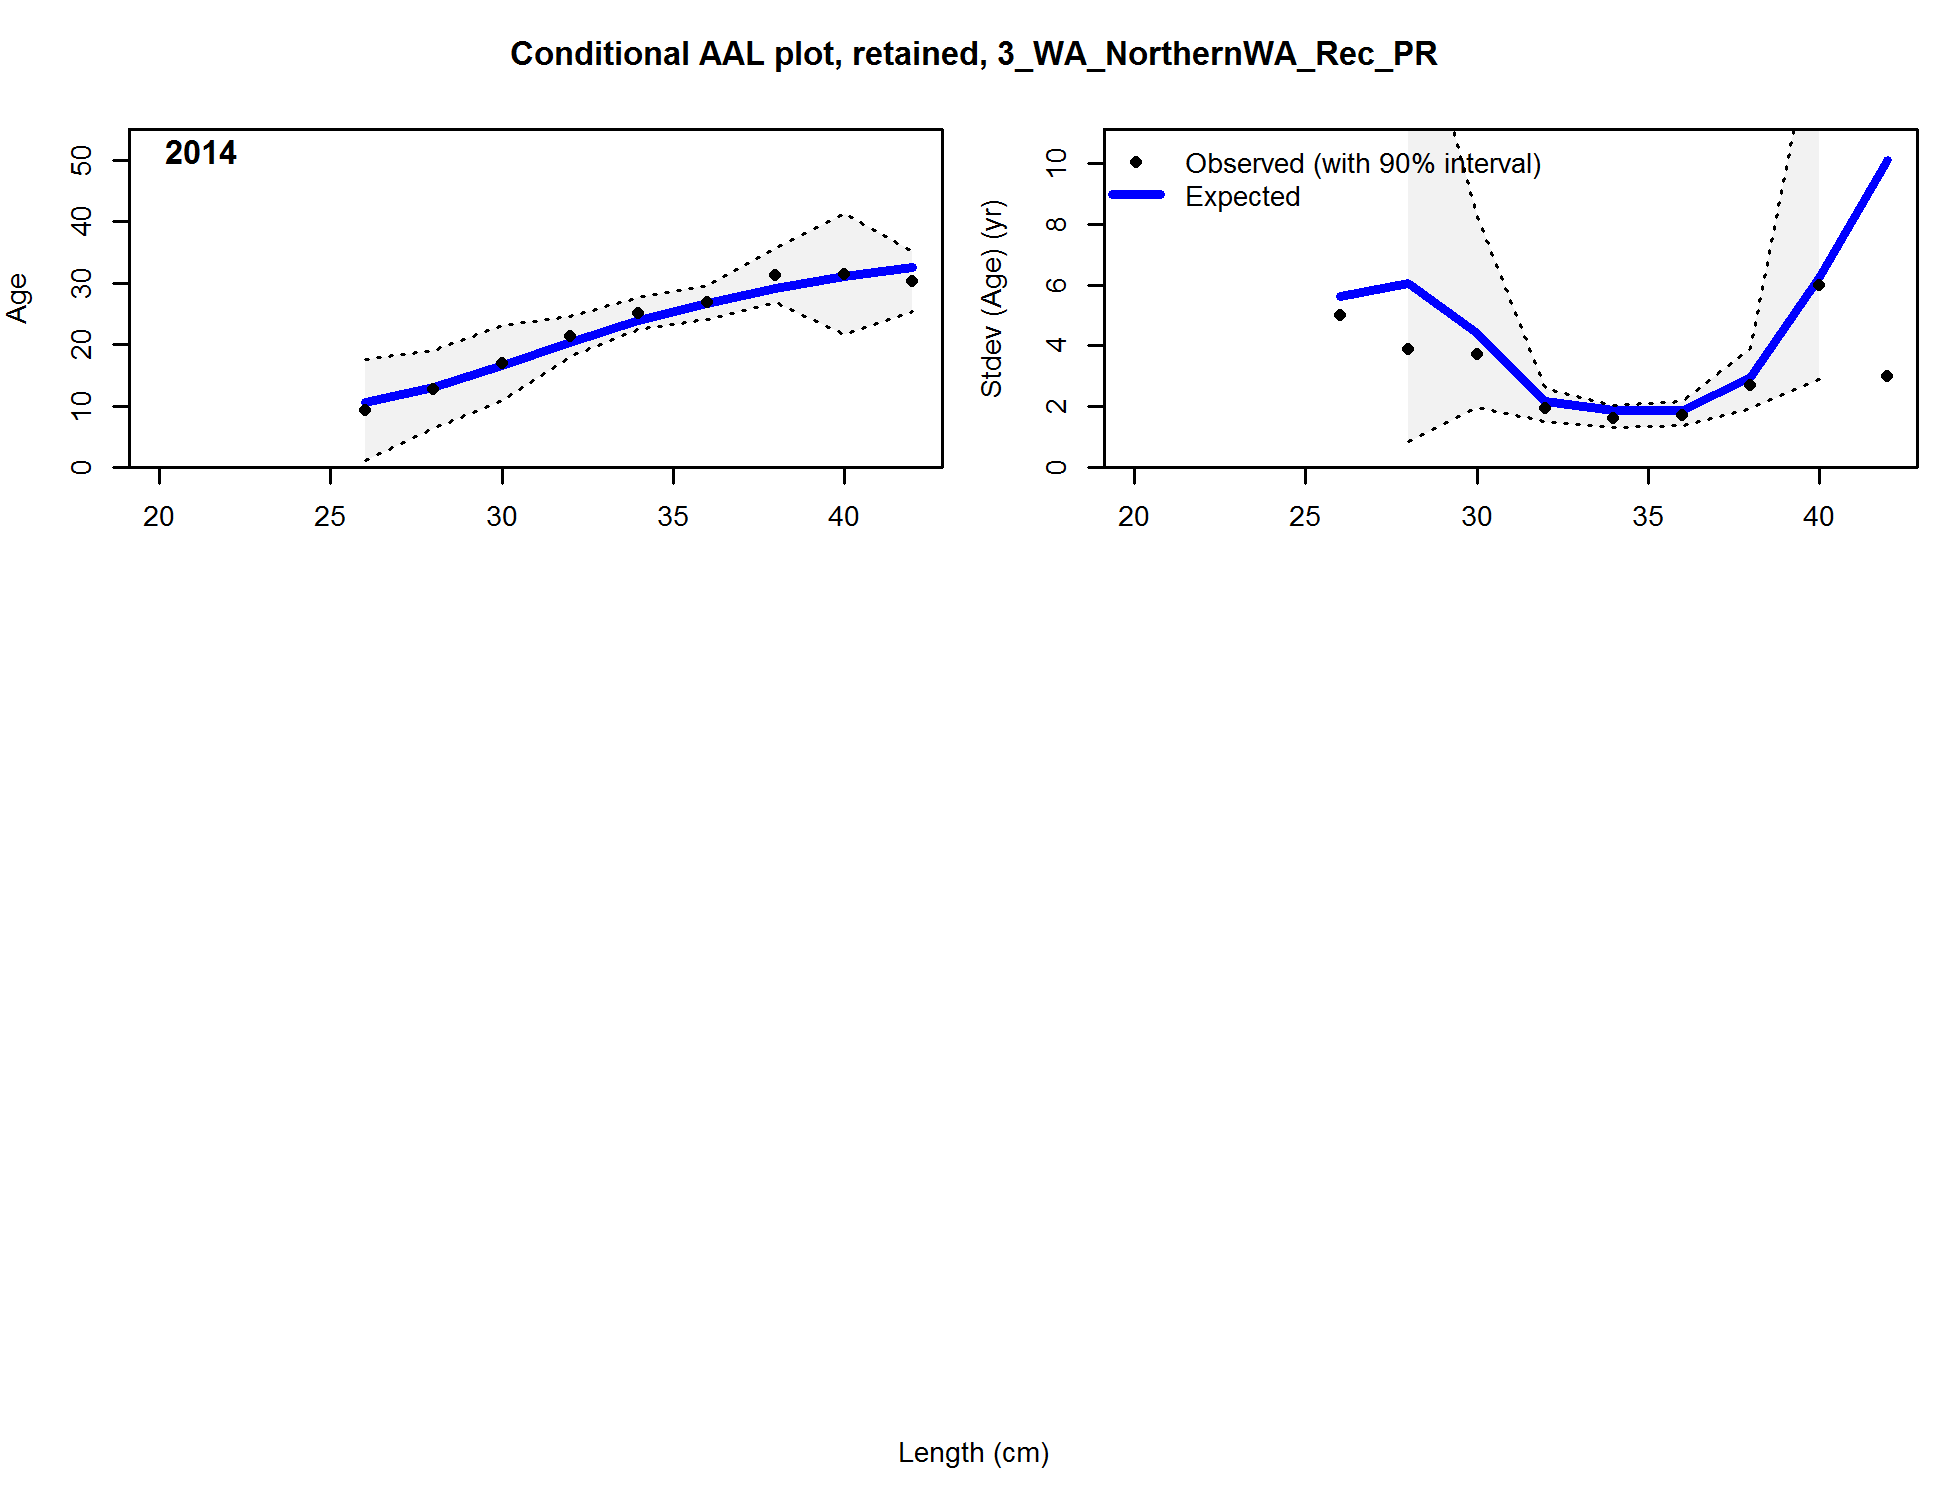
\includegraphics{./r4ss/plots_mod1/comp_condAALfit_Andre_plotsflt3mkt2_page6.png}

\begin{center} 

              Figure continued from previous page 

             \end{center}

\FloatBarrier

\FloatBarrier

\FloatBarrier
<!-- ***********h Likelihood profile FIGURES******************************* -->

\FloatBarrier
<!-- ********************************************************************** -->

\begin{figure}
\centering
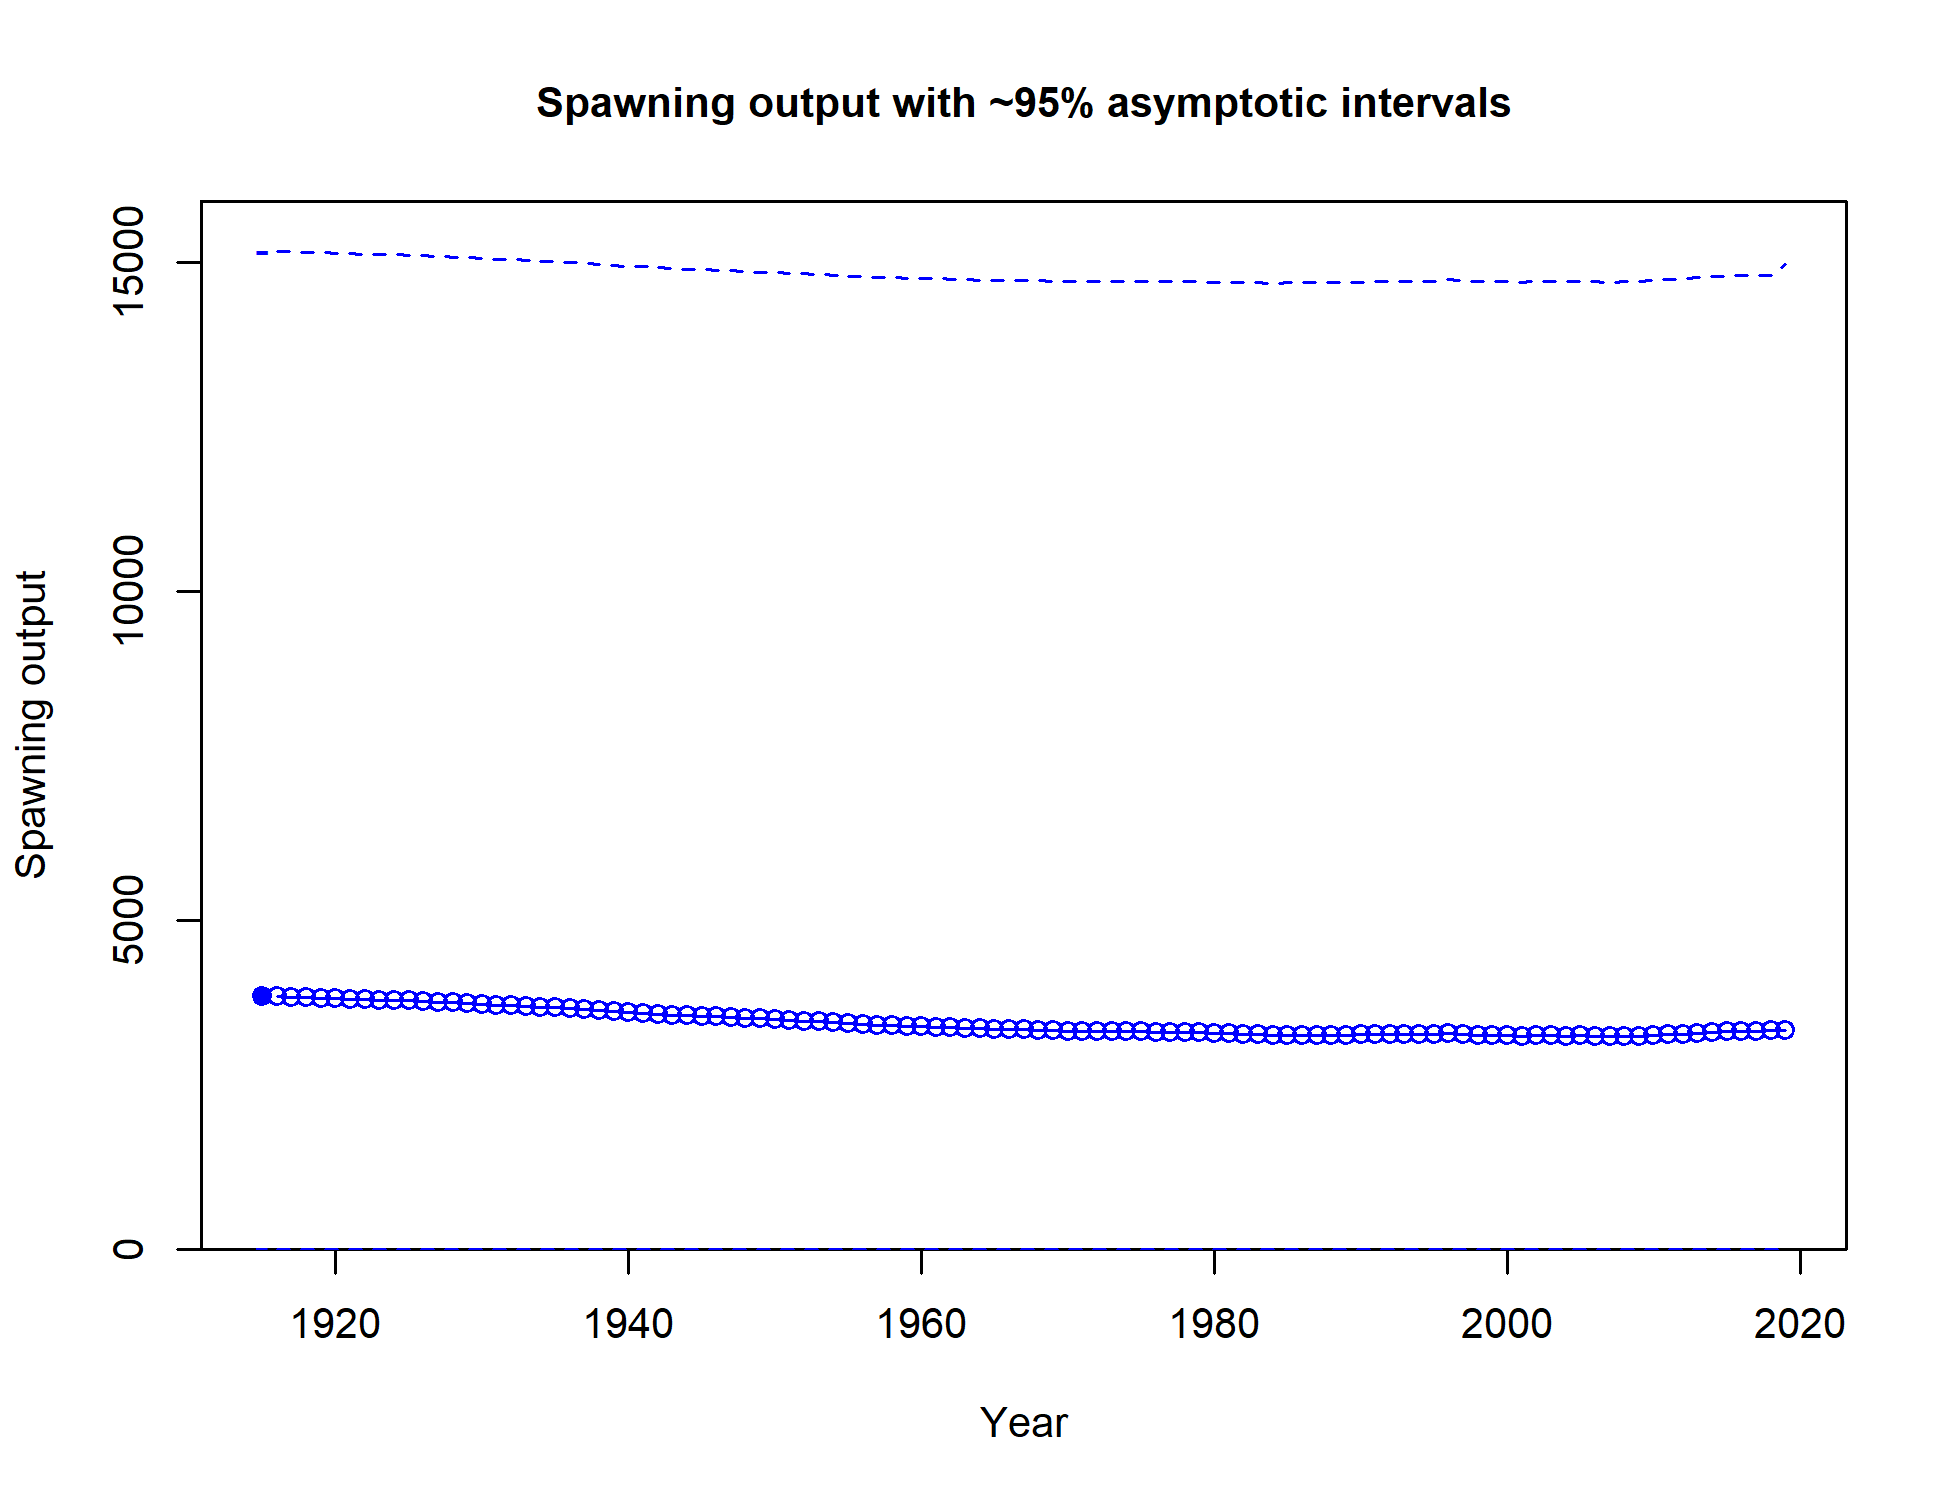
\includegraphics{r4ss/plots_mod1/ts7_Spawning_output_with_95_asymptotic_intervals_intervals.png}
\caption{Estimated spawning biomass (mt) with approximate 95\%
asymptotic intervals.
\label{fig:ts7_Spawning_biomass_(mt)_with_95_asymptotic_intervals_intervals}}
\end{figure}

\begin{figure}
\centering
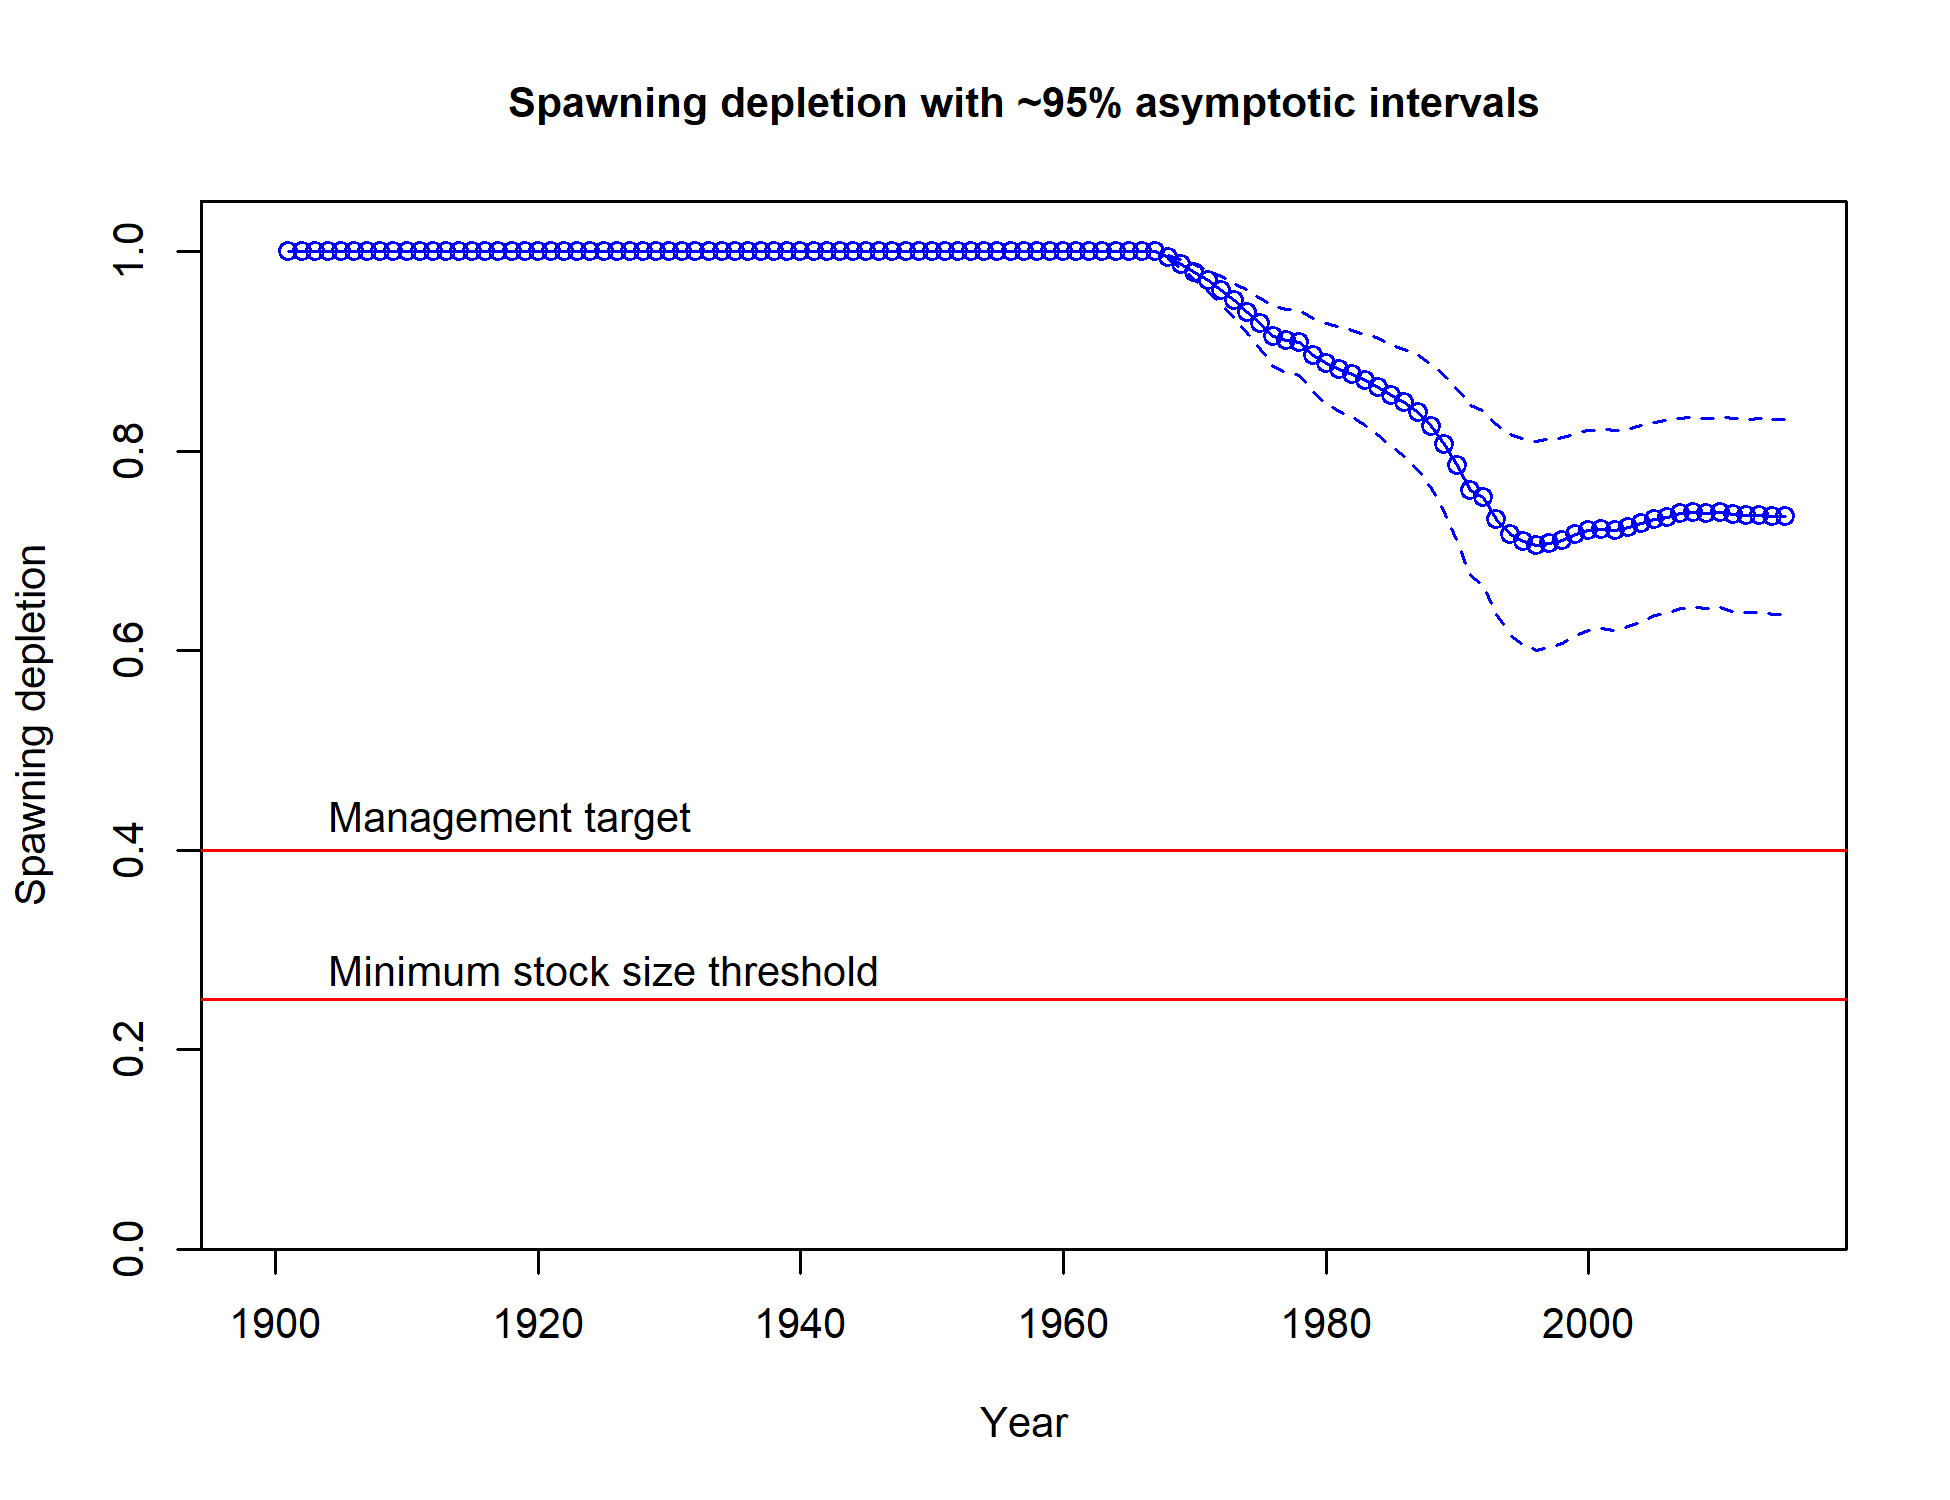
\includegraphics{r4ss/plots_mod1/ts9_Spawning_depletion_with_95_asymptotic_intervals_intervals.png}
\caption{Estimated spawning depletion with approximate 95\% asymptotic
intervals.
\label{fig:ts9_Spawning_depletion_with_95_asymptotic_intervals_intervals}}
\end{figure}

\begin{figure}
\centering
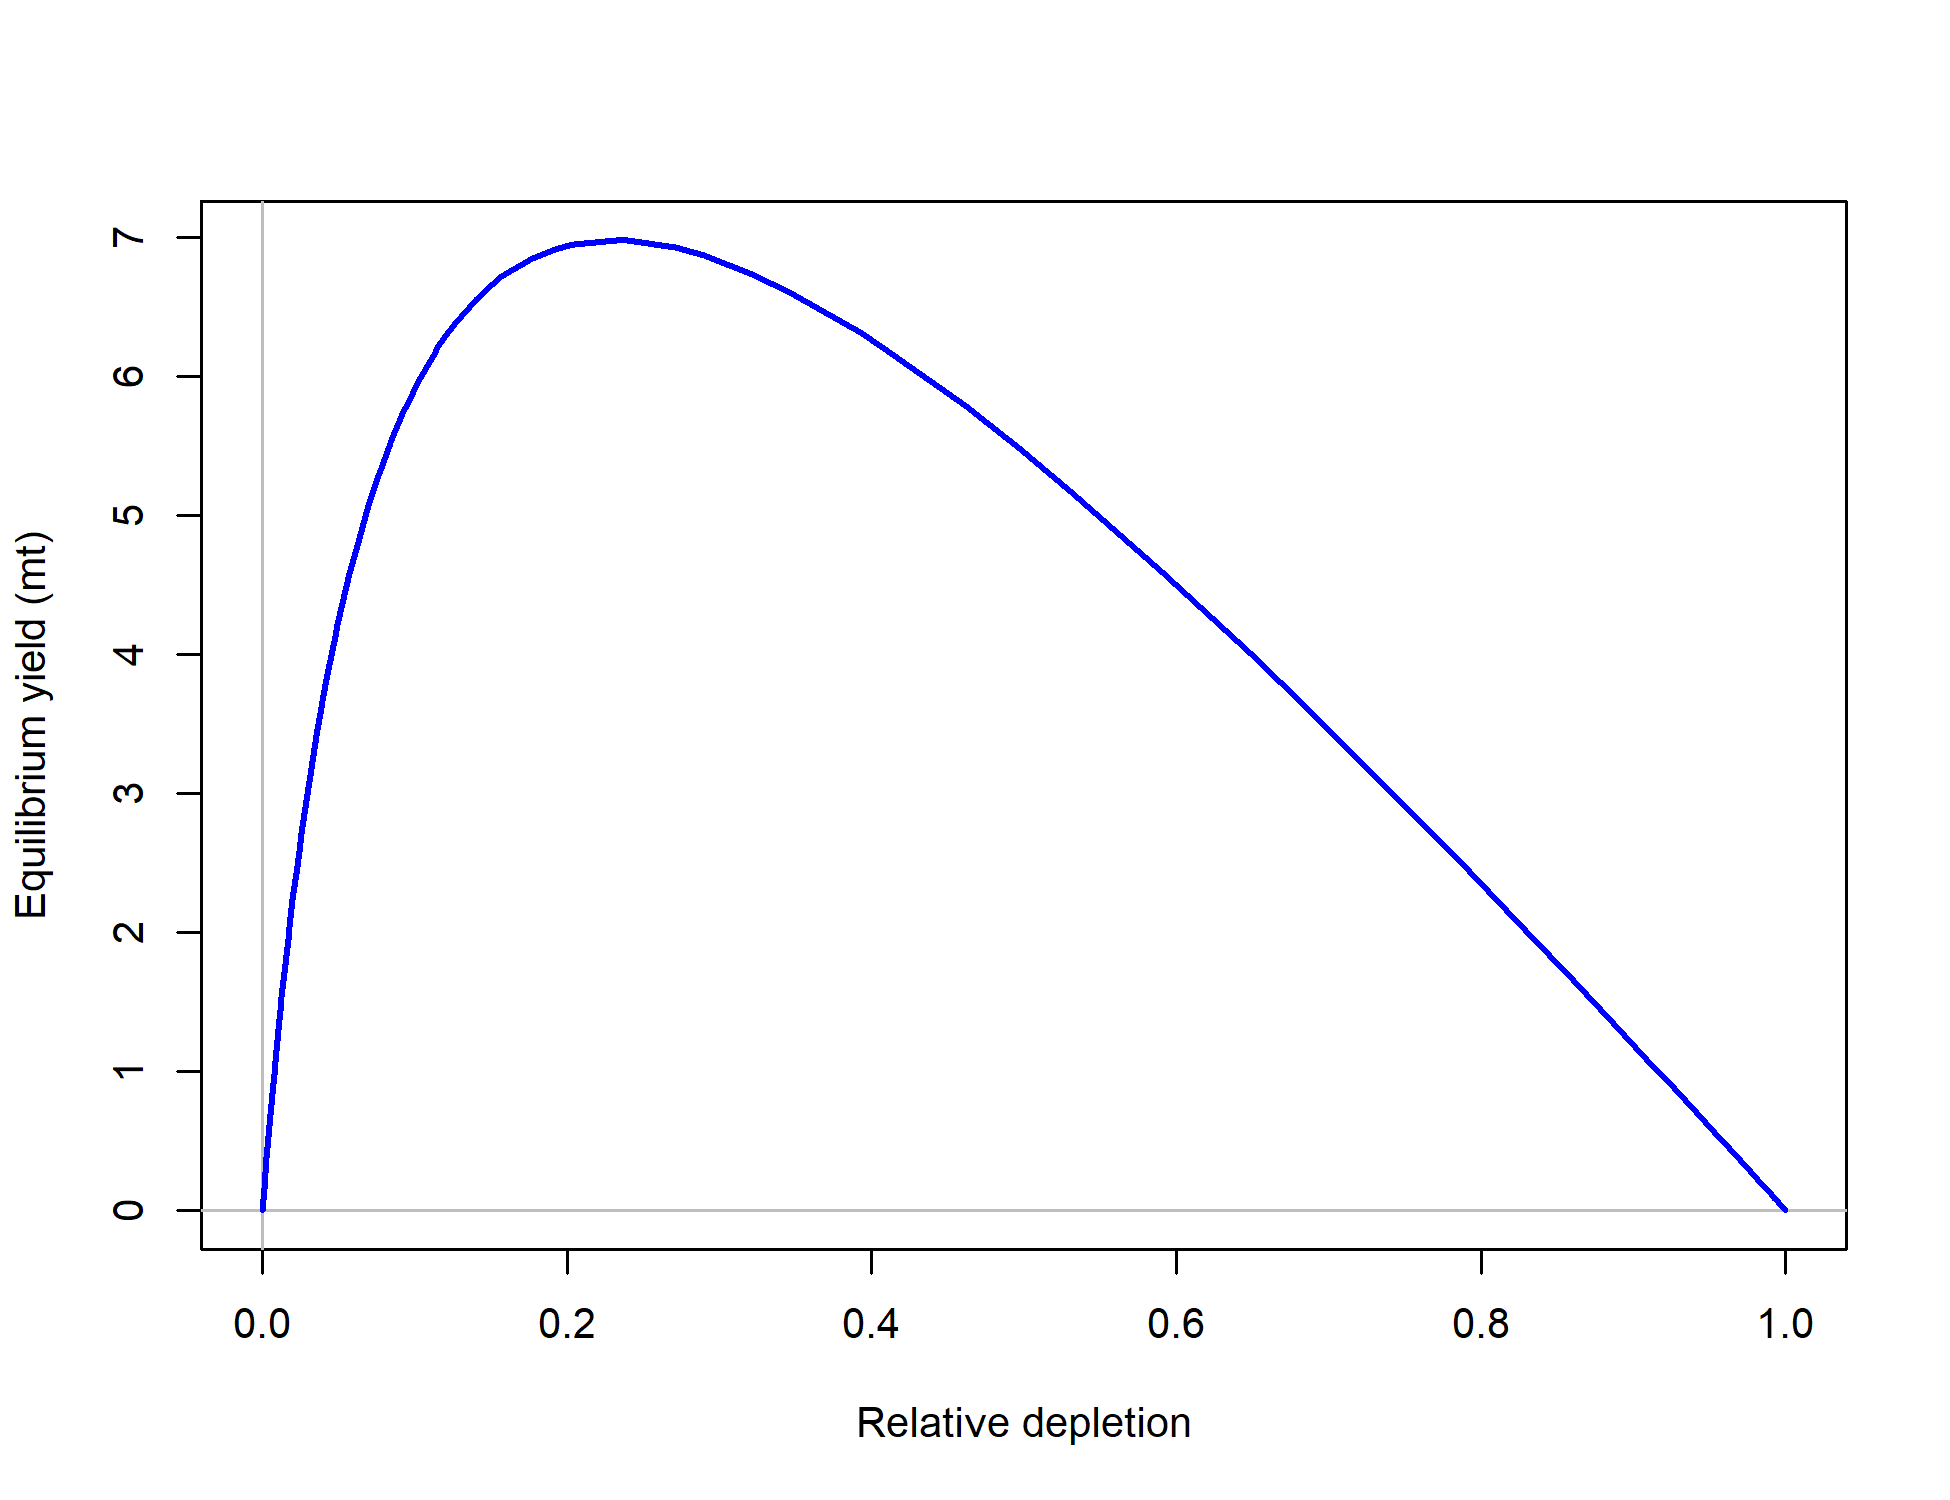
\includegraphics{r4ss/plots_mod1/yield1_yield_curve.png}
\caption{Equilibrium yield curve for the base case model. Values are
based on the 2014 fishery selectivity and with steepness fixed at 0.718.
\label{fig:yield1_yield_curve}}
\end{figure}

\FloatBarrier
<!-- ********************************************************************** -->

\FloatBarrier
\newpage

\section*{Appendix A. Detailed fits to length composition
data}\label{appendix-a.-detailed-fits-to-length-composition-data}
\addcontentsline{toc}{section}{Appendix A. Detailed fits to length
composition data}

\renewcommand{\thepage}{A-\arabic{page}}
\renewcommand{\thefigure}{A\arabic{figure}}

\setcounter{page}{1}

\begin{figure}
\centering
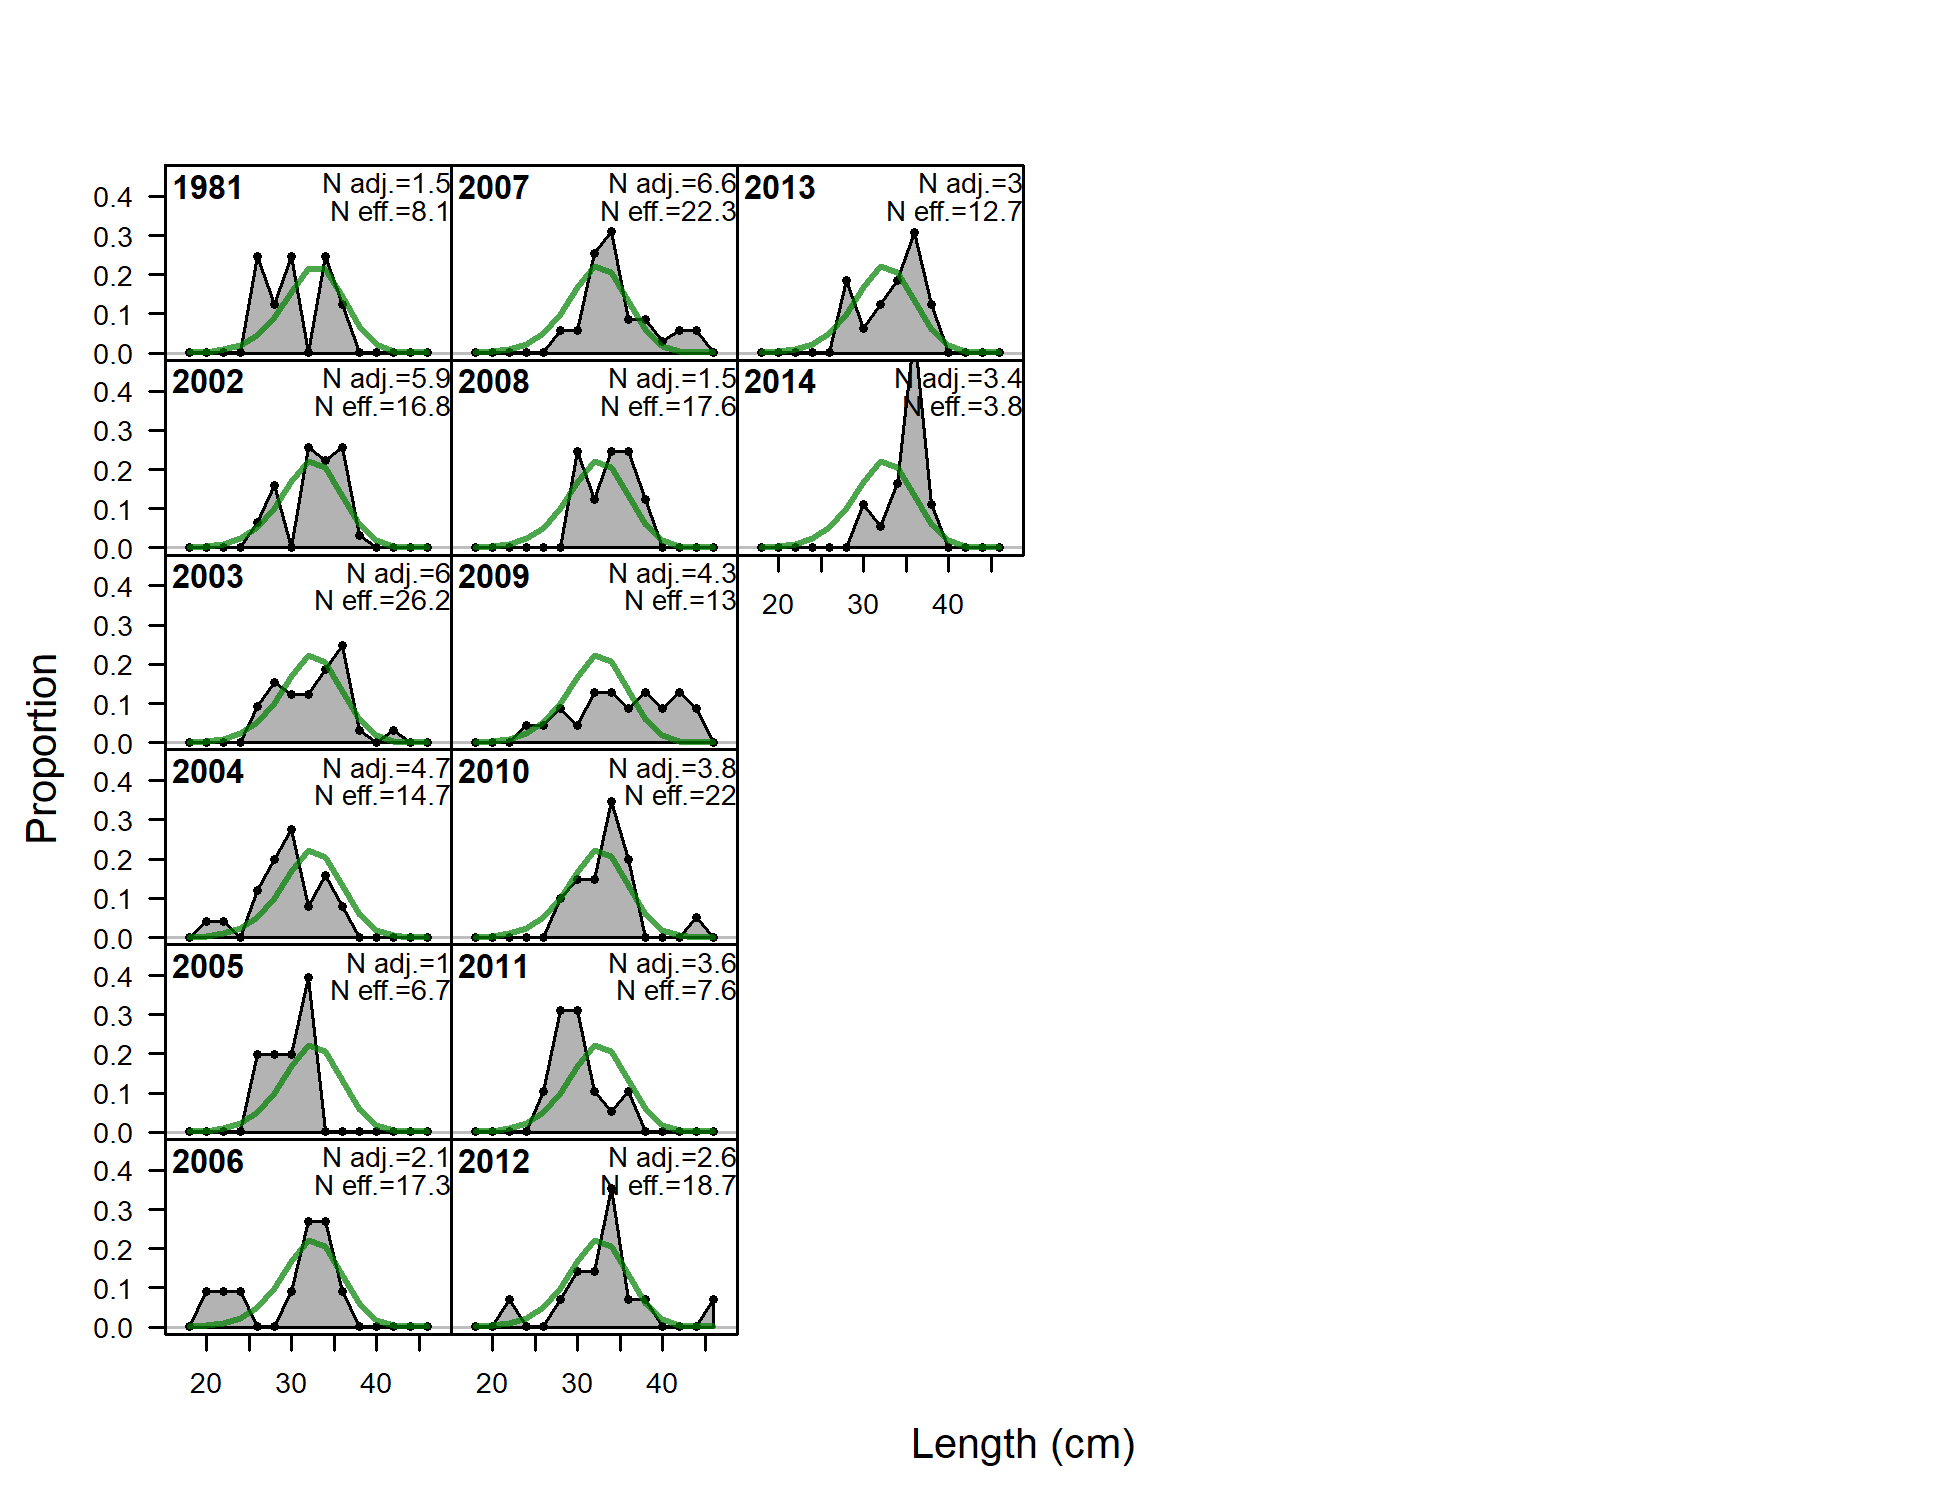
\includegraphics{./r4ss/plots_mod1/comp_lenfit_flt1mkt2.png}
\caption{Length comps, retained, 1\_WA\_SouthernWA\_Rec\_PCPR. `N adj.'
is the input sample size after data\_weighting adjustment. N eff. is the
calculated effective sample size used in the McAllister\_Iannelli tuning
method. \label{fig:mod1_1_comp_lenfit_flt1mkt2}}
\end{figure}

\begin{figure}
\centering
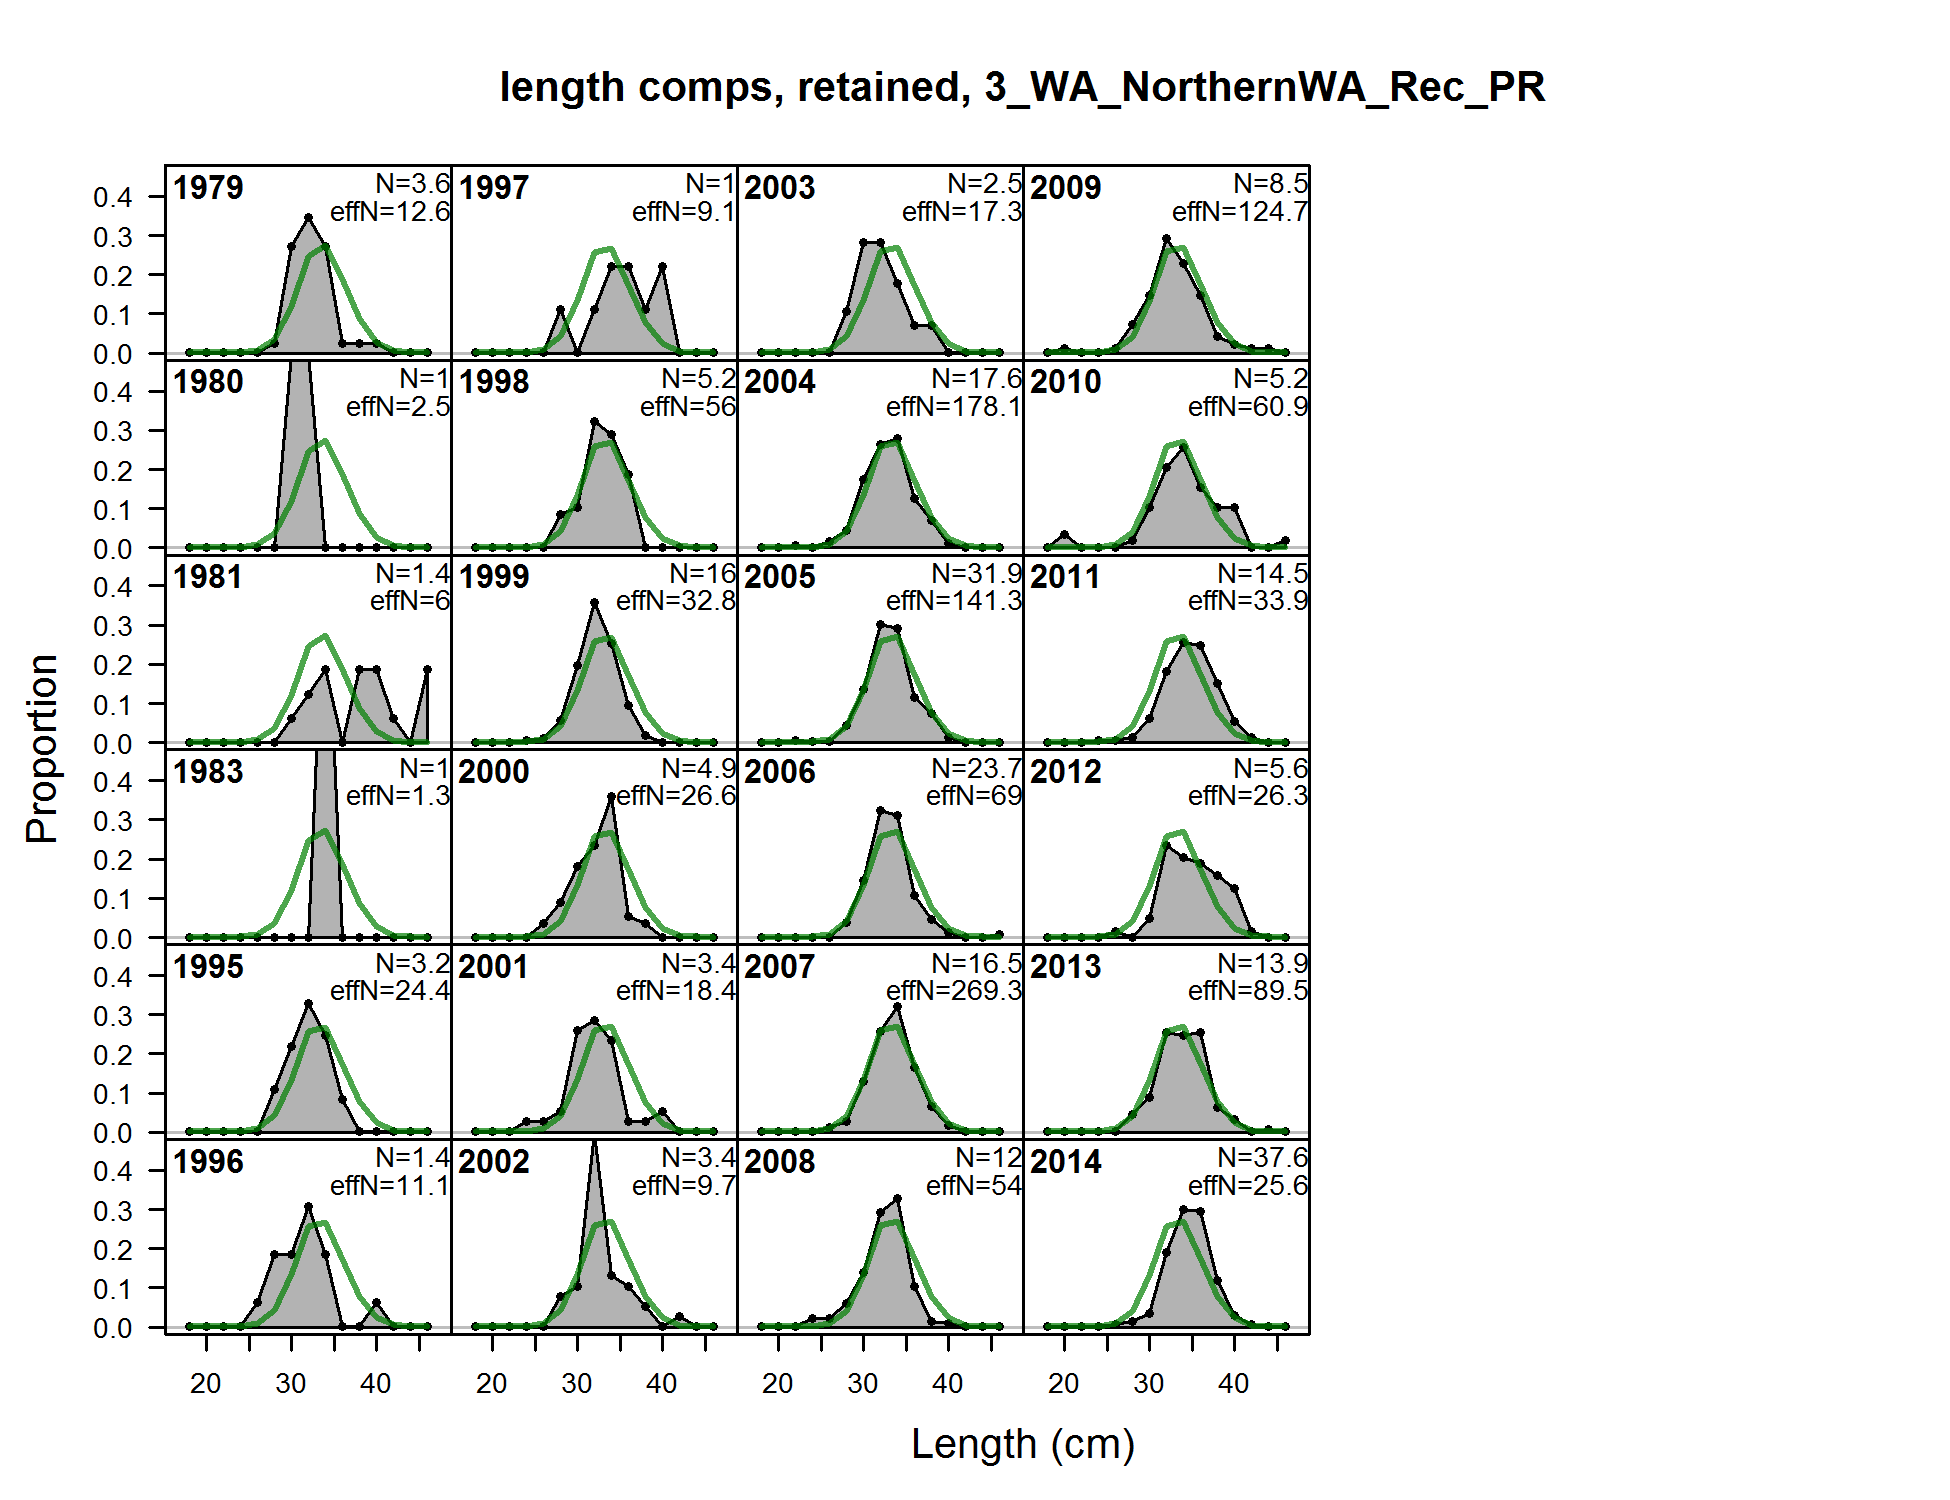
\includegraphics{./r4ss/plots_mod1/comp_lenfit_flt3mkt2.png}
\caption{Length comps, retained, 3\_WA\_NorthernWA\_Rec\_PR. `N adj.' is
the input sample size after data\_weighting adjustment. N eff. is the
calculated effective sample size used in the McAllister\_Iannelli tuning
method. \label{fig:mod1_2_comp_lenfit_flt3mkt2}}
\end{figure}

\newpage

\color{black}

\section*{References}\label{references}
\addcontentsline{toc}{section}{References}

\renewcommand{\thepage}{}

\hypertarget{refs}{}
\hypertarget{ref-vonB1938}{}
Bertalanffy, L. von. 1938. A quantitative theory of organic growth.
Human Biology \textbf{10}: 181--213.

\hypertarget{ref-Hamel2015}{}
Hamel, O. 2015. A method for calculating a meta-analytical prior for the
natural mortality rate using multiple life history correlates. ICES
Journal of Marine Science \textbf{72}: 62--69.

\hypertarget{ref-Love1987}{}
Love, M.S., Axell, B., Morris, P., Collins, R., and Brooks, A. 1987.
Life history and fishery of the California scorpionfish, \emph{Scorpaena
guttata}, within the Southern California Bight. Fishery Bulletin
\textbf{85}: 99--116.

\end{document}
